% Options for packages loaded elsewhere
% Options for packages loaded elsewhere
\PassOptionsToPackage{unicode}{hyperref}
\PassOptionsToPackage{hyphens}{url}
%
\documentclass[
  ignorenonframetext,
  brazilian,
]{beamer}
\newif\ifbibliography
\usepackage{pgfpages}
\setbeamertemplate{caption}[numbered]
\setbeamertemplate{caption label separator}{: }
\setbeamercolor{caption name}{fg=normal text.fg}
\beamertemplatenavigationsymbolsempty
% remove section numbering
\setbeamertemplate{part page}{
  \centering
  \begin{beamercolorbox}[sep=16pt,center]{part title}
    \usebeamerfont{part title}\insertpart\par
  \end{beamercolorbox}
}
\setbeamertemplate{section page}{
  \centering
  \begin{beamercolorbox}[sep=12pt,center]{section title}
    \usebeamerfont{section title}\insertsection\par
  \end{beamercolorbox}
}
\setbeamertemplate{subsection page}{
  \centering
  \begin{beamercolorbox}[sep=8pt,center]{subsection title}
    \usebeamerfont{subsection title}\insertsubsection\par
  \end{beamercolorbox}
}
% Prevent slide breaks in the middle of a paragraph
\widowpenalties 1 10000
\raggedbottom
\AtBeginPart{
  \frame{\partpage}
}
\AtBeginSection{
  \ifbibliography
  \else
    \frame{\sectionpage}
  \fi
}
\AtBeginSubsection{
  \frame{\subsectionpage}
}
\usepackage{iftex}
\ifPDFTeX
  \usepackage[T1]{fontenc}
  \usepackage[utf8]{inputenc}
  \usepackage{textcomp} % provide euro and other symbols
\else % if luatex or xetex
  \usepackage{unicode-math} % this also loads fontspec
  \defaultfontfeatures{Scale=MatchLowercase}
  \defaultfontfeatures[\rmfamily]{Ligatures=TeX,Scale=1}
\fi
\usepackage{lmodern}

\usetheme[]{Madrid}
\usecolortheme[]{default}
\ifPDFTeX\else
  % xetex/luatex font selection
\fi
% Use upquote if available, for straight quotes in verbatim environments
\IfFileExists{upquote.sty}{\usepackage{upquote}}{}
\IfFileExists{microtype.sty}{% use microtype if available
  \usepackage[]{microtype}
  \UseMicrotypeSet[protrusion]{basicmath} % disable protrusion for tt fonts
}{}
\makeatletter
\@ifundefined{KOMAClassName}{% if non-KOMA class
  \IfFileExists{parskip.sty}{%
    \usepackage{parskip}
  }{% else
    \setlength{\parindent}{0pt}
    \setlength{\parskip}{6pt plus 2pt minus 1pt}}
}{% if KOMA class
  \KOMAoptions{parskip=half}}
\makeatother


\usepackage{longtable,booktabs,array}
\newcounter{none} % for unnumbered tables
\usepackage{calc} % for calculating minipage widths
\usepackage{caption}
% Make caption package work with longtable
\makeatletter
\def\fnum@table{\tablename~\thetable}
\makeatother
\usepackage{graphicx}
\makeatletter
\newsavebox\pandoc@box
\newcommand*\pandocbounded[1]{% scales image to fit in text height/width
  \sbox\pandoc@box{#1}%
  \Gscale@div\@tempa{\textheight}{\dimexpr\ht\pandoc@box+\dp\pandoc@box\relax}%
  \Gscale@div\@tempb{\linewidth}{\wd\pandoc@box}%
  \ifdim\@tempb\p@<\@tempa\p@\let\@tempa\@tempb\fi% select the smaller of both
  \ifdim\@tempa\p@<\p@\scalebox{\@tempa}{\usebox\pandoc@box}%
  \else\usebox{\pandoc@box}%
  \fi%
}
% Set default figure placement to htbp
\def\fps@figure{htbp}
\makeatother


% definitions for citeproc citations
\NewDocumentCommand\citeproctext{}{}
\NewDocumentCommand\citeproc{mm}{%
  \begingroup\def\citeproctext{#2}\cite{#1}\endgroup}
\makeatletter
 % allow citations to break across lines
 \let\@cite@ofmt\@firstofone
 % avoid brackets around text for \cite:
 \def\@biblabel#1{}
 \def\@cite#1#2{{#1\if@tempswa , #2\fi}}
\makeatother
\newlength{\cslhangindent}
\setlength{\cslhangindent}{1.5em}
\newlength{\csllabelwidth}
\setlength{\csllabelwidth}{3em}
\newenvironment{CSLReferences}[2] % #1 hanging-indent, #2 entry-spacing
 {\begin{list}{}{%
  \setlength{\itemindent}{0pt}
  \setlength{\leftmargin}{0pt}
  \setlength{\parsep}{0pt}
  % turn on hanging indent if param 1 is 1
  \ifodd #1
   \setlength{\leftmargin}{\cslhangindent}
   \setlength{\itemindent}{-1\cslhangindent}
  \fi
  % set entry spacing
  \setlength{\itemsep}{#2\baselineskip}}}
 {\end{list}}
\usepackage{calc}
\newcommand{\CSLBlock}[1]{\hfill\break\parbox[t]{\linewidth}{\strut\ignorespaces#1\strut}}
\newcommand{\CSLLeftMargin}[1]{\parbox[t]{\csllabelwidth}{\strut#1\strut}}
\newcommand{\CSLRightInline}[1]{\parbox[t]{\linewidth - \csllabelwidth}{\strut#1\strut}}
\newcommand{\CSLIndent}[1]{\hspace{\cslhangindent}#1}

\ifLuaTeX
\usepackage[bidi=basic,shorthands=off]{babel}
\else
\usepackage[bidi=default,shorthands=off]{babel}
\fi
\ifLuaTeX
  \usepackage{selnolig} % disable illegal ligatures
\fi


\setlength{\emergencystretch}{3em} % prevent overfull lines

\providecommand{\tightlist}{%
  \setlength{\itemsep}{0pt}\setlength{\parskip}{0pt}}



 


\makeatletter
\@ifpackageloaded{caption}{}{\usepackage{caption}}
\AtBeginDocument{%
\ifdefined\contentsname
  \renewcommand*\contentsname{Índice}
\else
  \newcommand\contentsname{Índice}
\fi
\ifdefined\listfigurename
  \renewcommand*\listfigurename{Lista de Figuras}
\else
  \newcommand\listfigurename{Lista de Figuras}
\fi
\ifdefined\listtablename
  \renewcommand*\listtablename{Lista de Tabelas}
\else
  \newcommand\listtablename{Lista de Tabelas}
\fi
\ifdefined\figurename
  \renewcommand*\figurename{Figura}
\else
  \newcommand\figurename{Figura}
\fi
\ifdefined\tablename
  \renewcommand*\tablename{Tabela}
\else
  \newcommand\tablename{Tabela}
\fi
}
\@ifpackageloaded{float}{}{\usepackage{float}}
\floatstyle{ruled}
\@ifundefined{c@chapter}{\newfloat{codelisting}{h}{lop}}{\newfloat{codelisting}{h}{lop}[chapter]}
\floatname{codelisting}{Listagem}
\newcommand*\listoflistings{\listof{codelisting}{Lista de Listagens}}
\makeatother
\makeatletter
\makeatother
\makeatletter
\@ifpackageloaded{caption}{}{\usepackage{caption}}
\@ifpackageloaded{subcaption}{}{\usepackage{subcaption}}
\makeatother

\usepackage{bookmark}
\IfFileExists{xurl.sty}{\usepackage{xurl}}{} % add URL line breaks if available
\urlstyle{same}
\hypersetup{
  pdftitle={Mortalidade e Internações na Primeira Infância},
  pdflang={pt-BR},
  hidelinks,
  pdfcreator={LaTeX via pandoc}}


\title{\texorpdfstring{Mortalidade e Internações na Primeira
Infância}{Mortalidade e Internações na Primeira Infância}}
\subtitle{\texorpdfstring{Evolução do Projeto}{Evolução do Projeto}}
\author{}
\date{2026-06-01}

\begin{document}
\frame{\titlepage}


\begin{frame}{Dados e abordagem}
\protect\phantomsection\label{dados-e-abordagem}
\textbf{Fontes de dados:}\\

\begin{itemize}
\tightlist
\item
  SIM --- Sistema de Informações sobre Mortalidade\\
\item
  SIH/SUS --- Sistema de Informações Hospitalares do SUS\\
\item
  SINASC --- Sistema de Informações sobre Nascidos Vivos\\
\end{itemize}

\textbf{Período:} 2015 a 2024

(Brasil. Ministério da Saúde. Secretaria de Vigilância em Saúde 2024)
\end{frame}

\begin{frame}{Dados e abordagem}
\protect\phantomsection\label{dados-e-abordagem-1}
\textbf{Faixas etárias:}\\

\begin{itemize}
\tightlist
\item
  Visão geral:\\

  \begin{itemize}
  \tightlist
  \item
    Menos de 1 ano;\\
  \item
    De 1 ano até menos que cinco anos;\\
  \item
    5 e 6 anos.\\
  \end{itemize}
\item
  Visão detalhada:\\

  \begin{itemize}
  \tightlist
  \item
    Neonatal:\\

    \begin{itemize}
    \tightlist
    \item
      Neonatal precoce: 0--6 dias;\\
    \item
      Neonatal tardia: 7--27 dias;\\
    \item
      Pós-neonatal: 28 dias a \textless1 ano.\\
    \end{itemize}
  \item
    Crianças:\\

    \begin{itemize}
    \tightlist
    \item
      1 a \textless{} 2 anos;\\
    \item
      2 a \textless{} 5 anos;\\
    \item
      5 e 6 anos.
    \end{itemize}
  \end{itemize}
\end{itemize}

(United Nations Inter-Agency Group for Child Mortality Estimation (UN
IGME) 2025), (Brasil. Ministério da Saúde 2026), (França e Lansky 2009)
\end{frame}

\begin{frame}{Dados e abordagem}
\protect\phantomsection\label{dados-e-abordagem-2}
\begin{itemize}
\item
  \textbf{Unidade de medida das taxas:} as taxas são expressas por 1.000
  nascidos vivos da SINASC\\
\item
  \textbf{Polos de referência:} os diagnósticos são segmentados em
  grupos de alta complexidade:\\

  \begin{itemize}
  \tightlist
  \item
    Oncologia;\\
  \item
    Cardiopatias congênitas;\\
  \item
    Malformações;\\
  \item
    Doenças do sistema nervoso, metabólicas ou genéticas.\\
  \end{itemize}
\item
  \textbf{Afecções perinatais} são analisadas em separado, pois parte do
  evento perinatal recebido nos polos reflete o local de parto e não o
  deslocamento da criança em busca de tratamento.\\
\item
  \textbf{Referência terapêutica} de alta complexidade \emph{sem}
  perinatal é o fluxo para identificar centros de referência e vazios
  assistenciais.\\
\end{itemize}
\end{frame}

\begin{frame}{Evolução da Mortalidade na Primeira Infância}
\protect\phantomsection\label{evoluuxe7uxe3o-da-mortalidade-na-primeira-infuxe2ncia}
\begin{itemize}
\tightlist
\item
  Fazer gráfico de taxa de mortalidade e mortalidade por milhares para
  menos que um ano, 1 a menos que 5 anos e 5 e 6 anos, como na visão
  geral; referência:
  https://data.unicef.org/resources/levels-and-trends-in-child-mortality-2024/
\end{itemize}
\end{frame}

\begin{frame}{Evolução da Mortalidade no Neonatal}
\protect\phantomsection\label{evoluuxe7uxe3o-da-mortalidade-no-neonatal}
\begin{itemize}
\tightlist
\item
  Fazer gráfico de taxa de mortalidade e mortalidade por milhares para
  neotanal por neonatal precoce, neonatal tardia, pós-neonatal
\end{itemize}
\end{frame}

\begin{frame}{Evolução da Mortalidade para Crianças}
\protect\phantomsection\label{evoluuxe7uxe3o-da-mortalidade-para-crianuxe7as}
\begin{itemize}
\tightlist
\item
  Fazer gráfico de taxa de mortalidade e mortalidade por milhares para
  crianças: 1 a \textless{} 2 anos, 2 a \textless{} 5 anos e 5 e 6 anos
\end{itemize}
\end{frame}

\begin{frame}{Causas de Mortalidade}
\protect\phantomsection\label{causas-de-mortalidade}
\begin{figure}[H]

{\centering 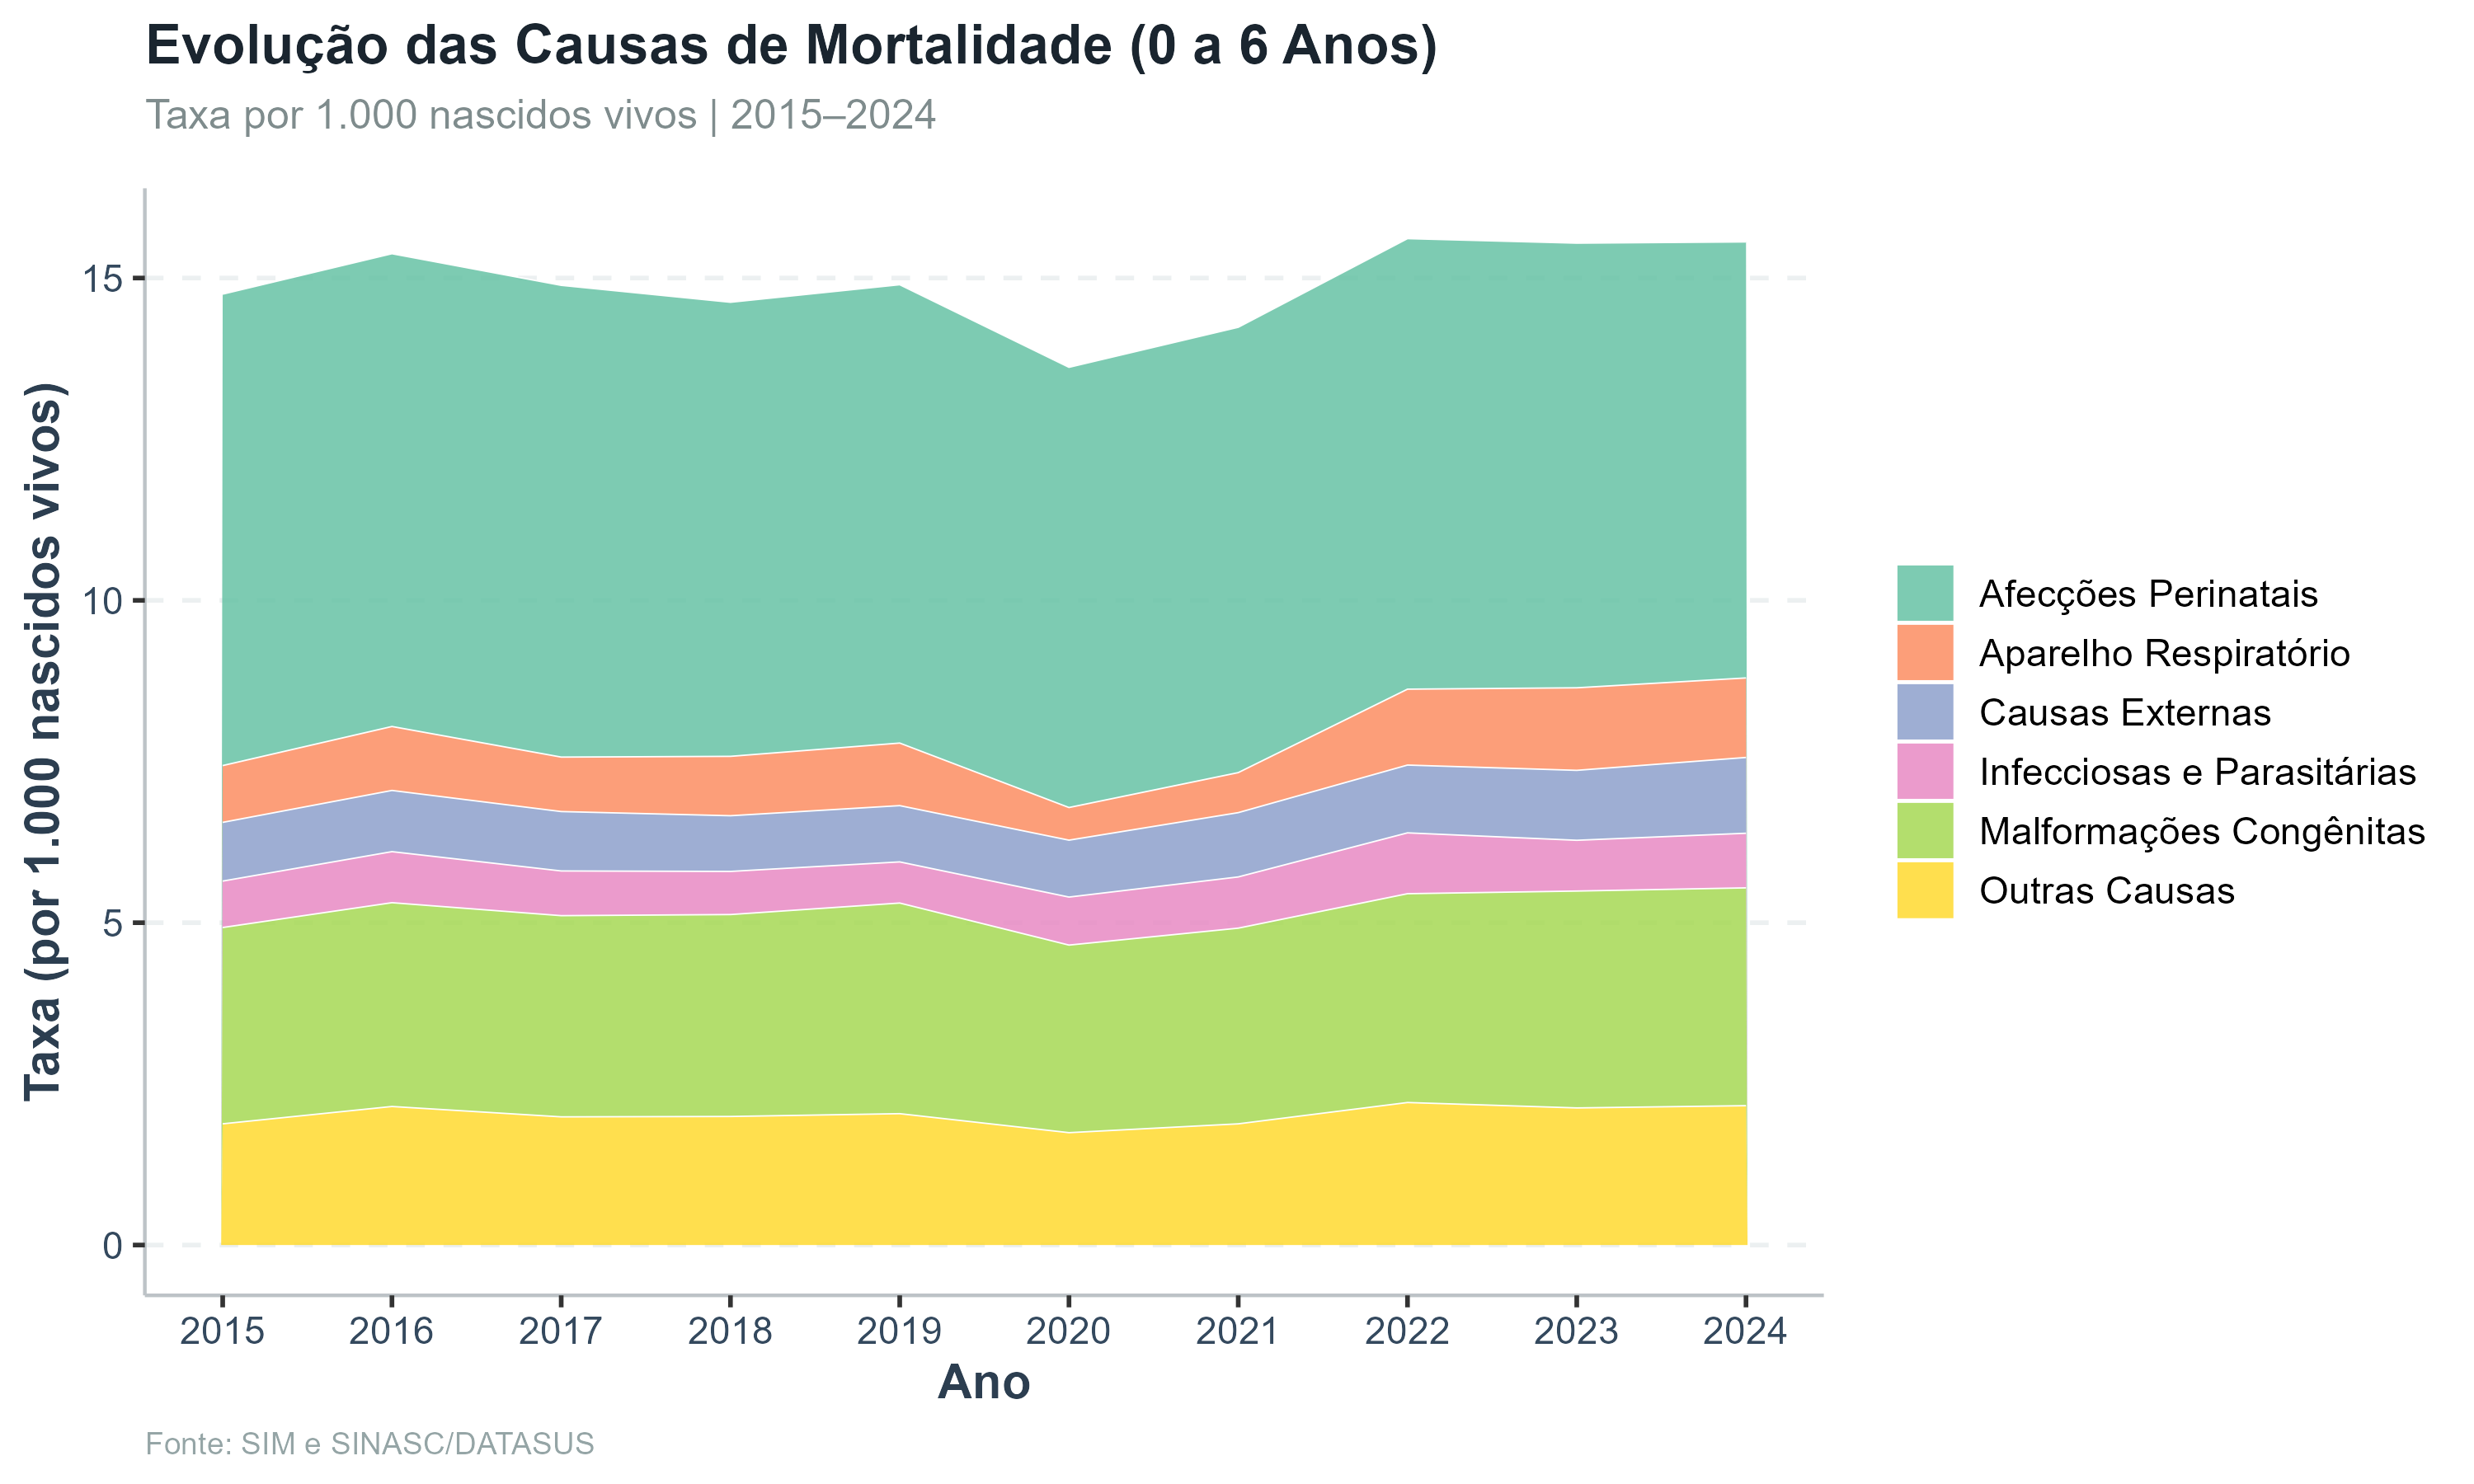
\includegraphics[width=0.9\linewidth,height=\textheight,keepaspectratio]{../outputs/SIM/Fig02_Evolucao_Causas_Taxa.png}

}

\caption{Evolução das causas de mortalidade, 2015--2024}

\end{figure}%
\end{frame}

\begin{frame}{Causas de Mortalidade por Faixa Etária}
\protect\phantomsection\label{causas-de-mortalidade-por-faixa-etuxe1ria}
\begin{figure}[H]

{\centering 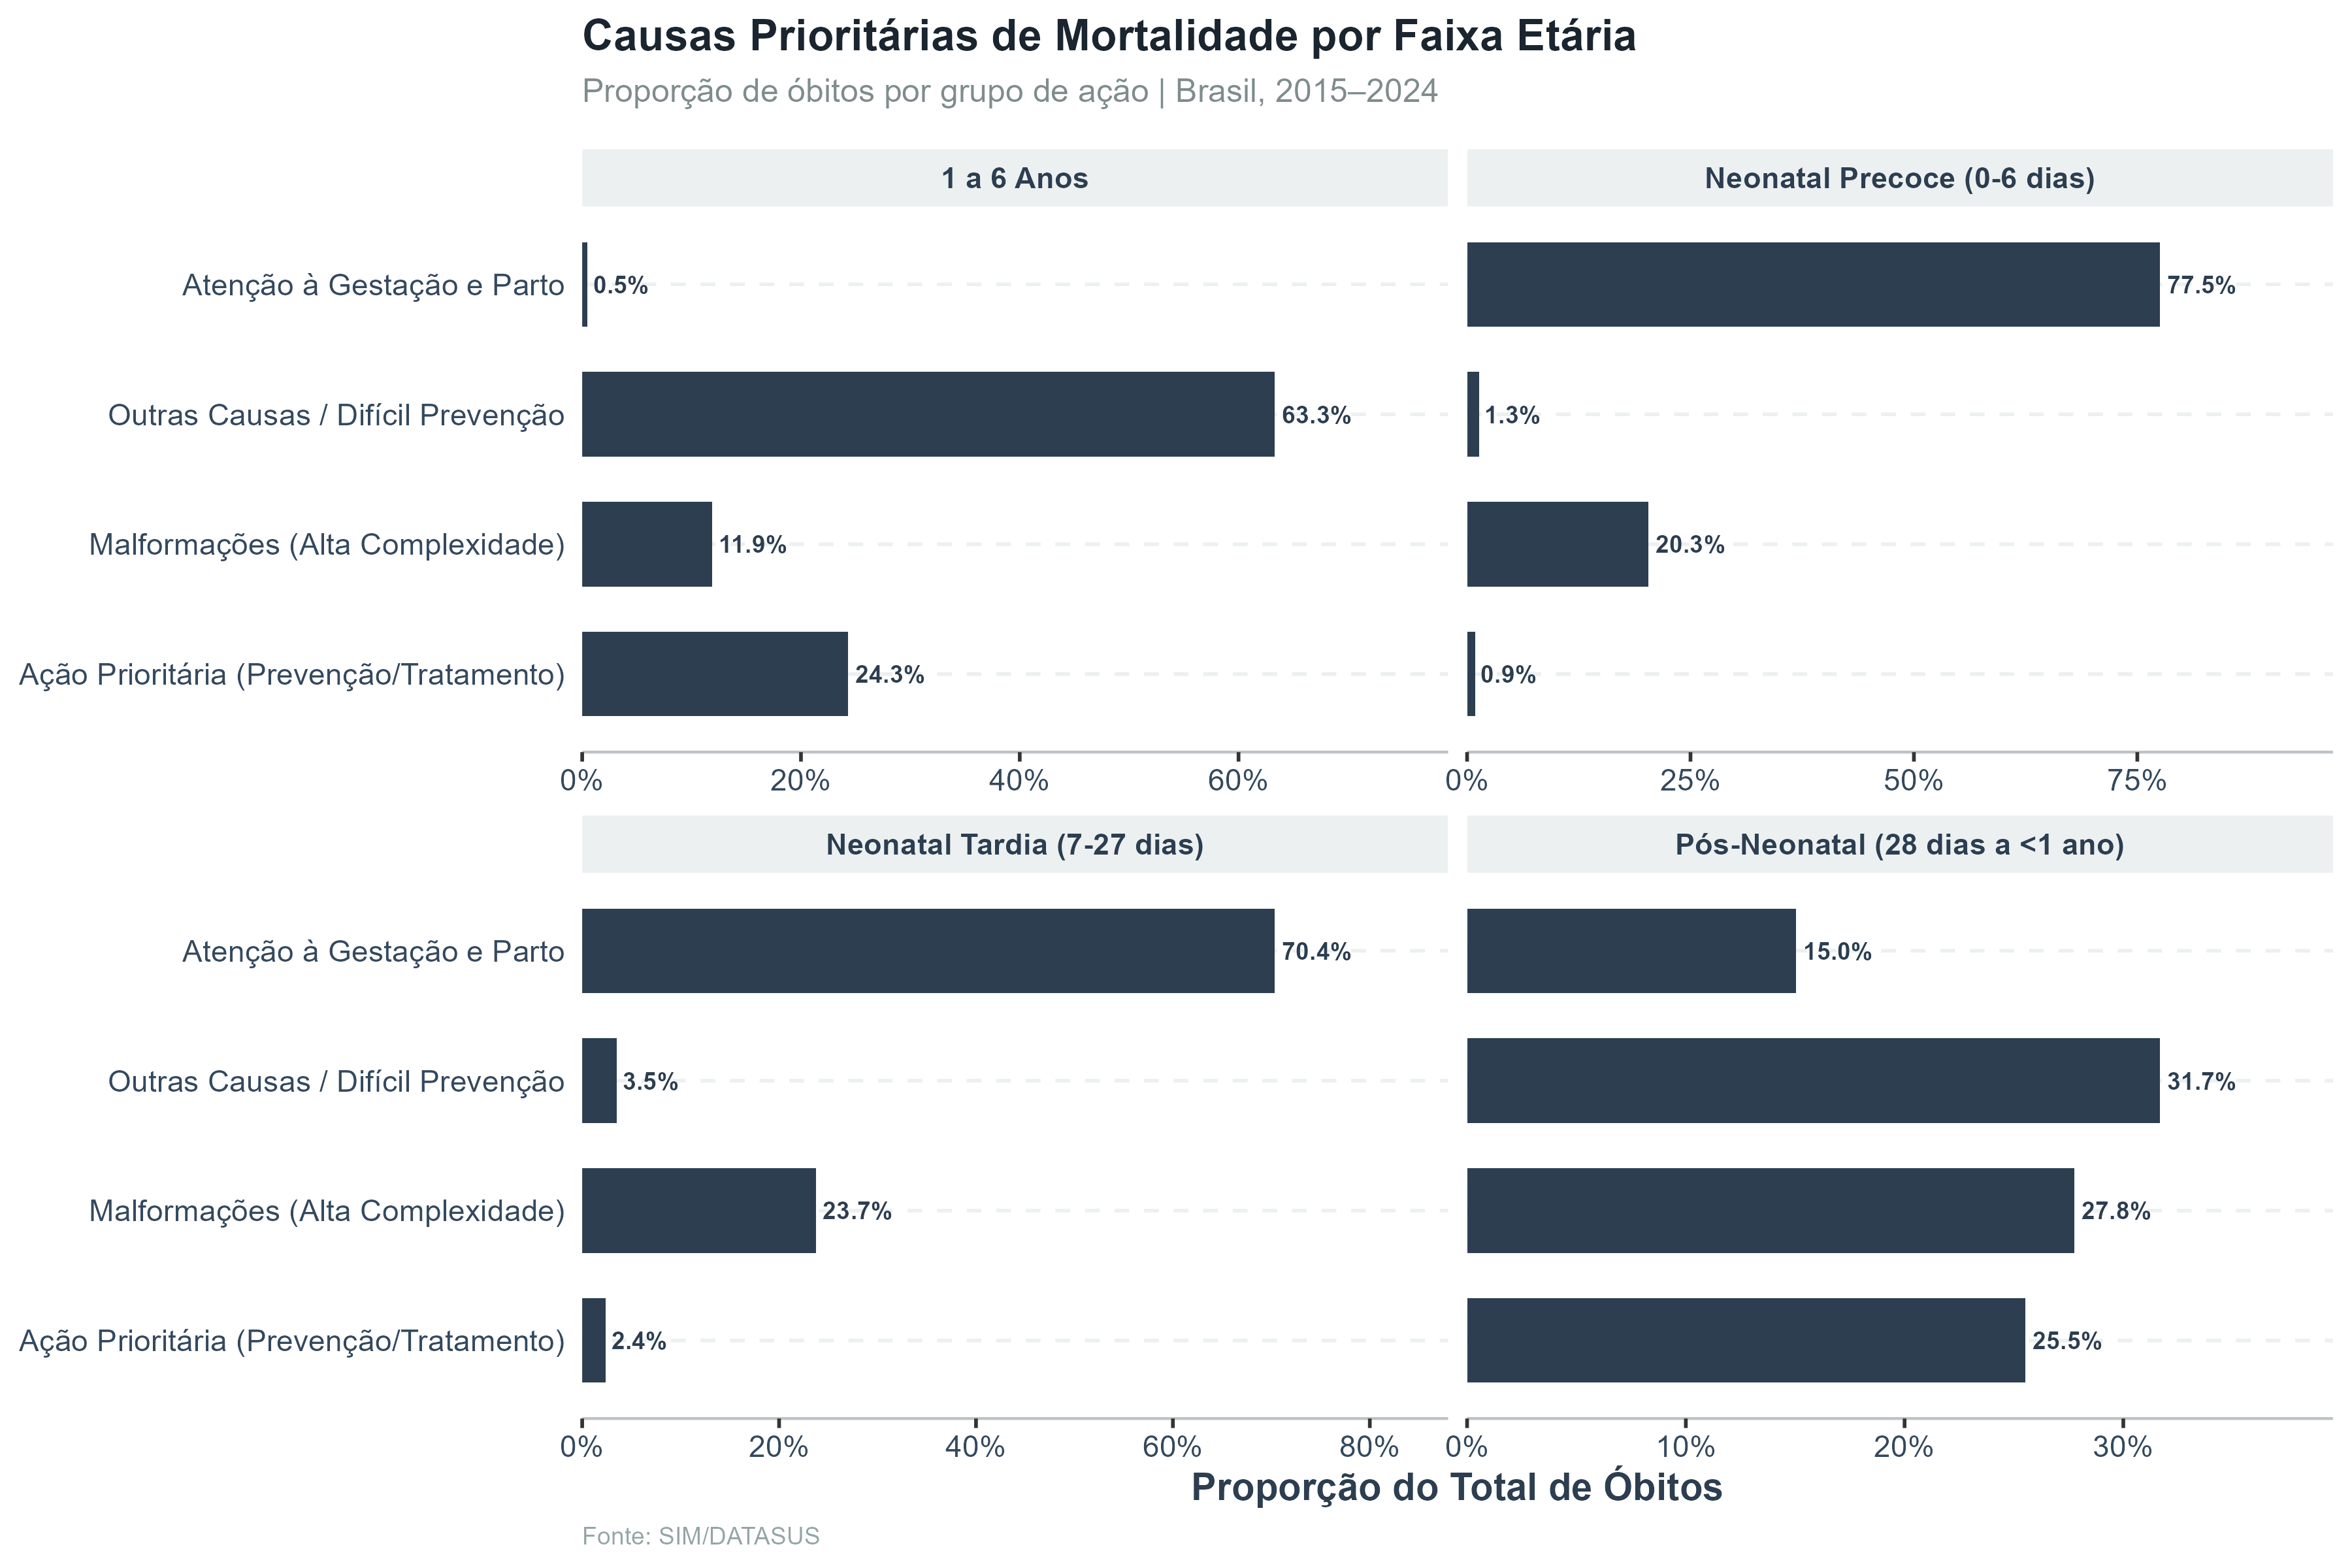
\includegraphics[width=0.9\linewidth,height=\textheight,keepaspectratio]{../outputs/SIM/Fig03_Causas_Prioritarias_por_Faixa.png}

}

\caption{Causas prioritárias de mortalidade, 2015--2024}

\end{figure}%
\end{frame}

\begin{frame}{Análise Espacial e Desigualdades Regionais da Mortalidade}
\protect\phantomsection\label{anuxe1lise-espacial-e-desigualdades-regionais-da-mortalidade}
\begin{figure}[H]

{\centering 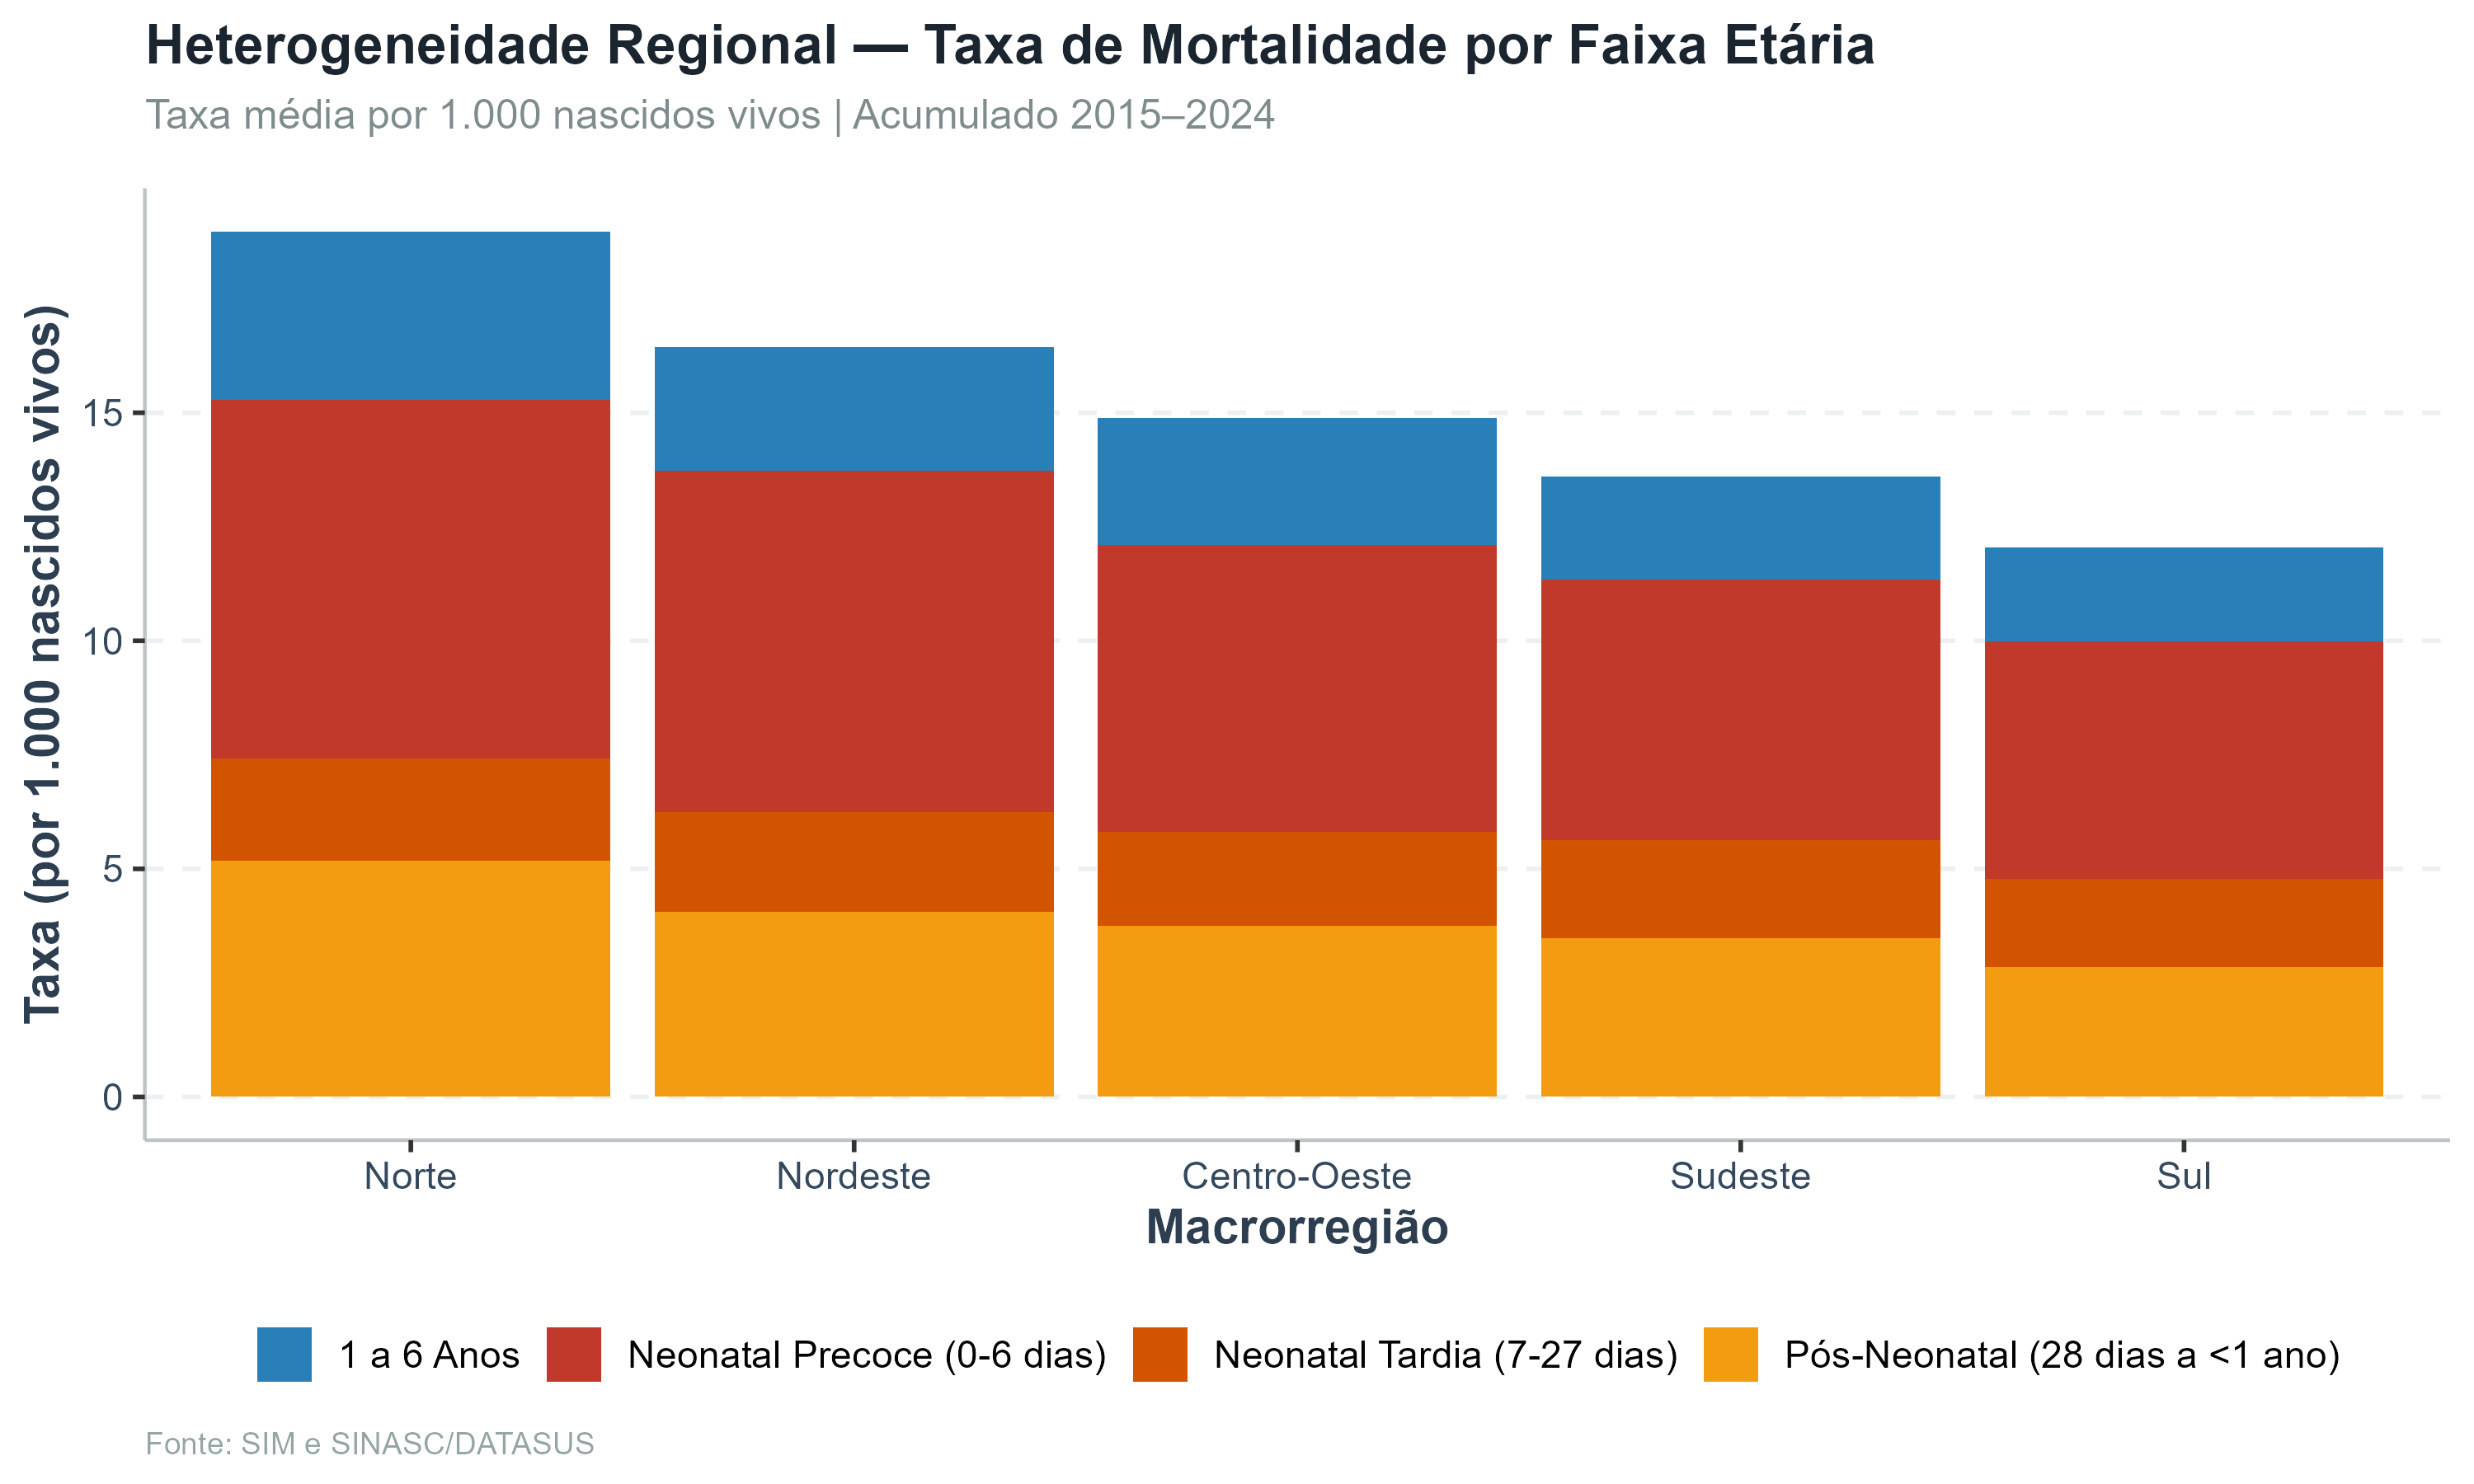
\includegraphics[width=0.9\linewidth,height=\textheight,keepaspectratio]{../outputs/SIM/Fig04_Heterogeneidade_Macro_Taxa.png}

}

\caption{Heterogeneidade Regional da Taxa de Mortalidade, 2015--2024}

\end{figure}%
\end{frame}

\begin{frame}{Análise Espacial e Desigualdades Regionais da Mortalidade}
\protect\phantomsection\label{anuxe1lise-espacial-e-desigualdades-regionais-da-mortalidade-1}
\begin{figure}[H]

{\centering 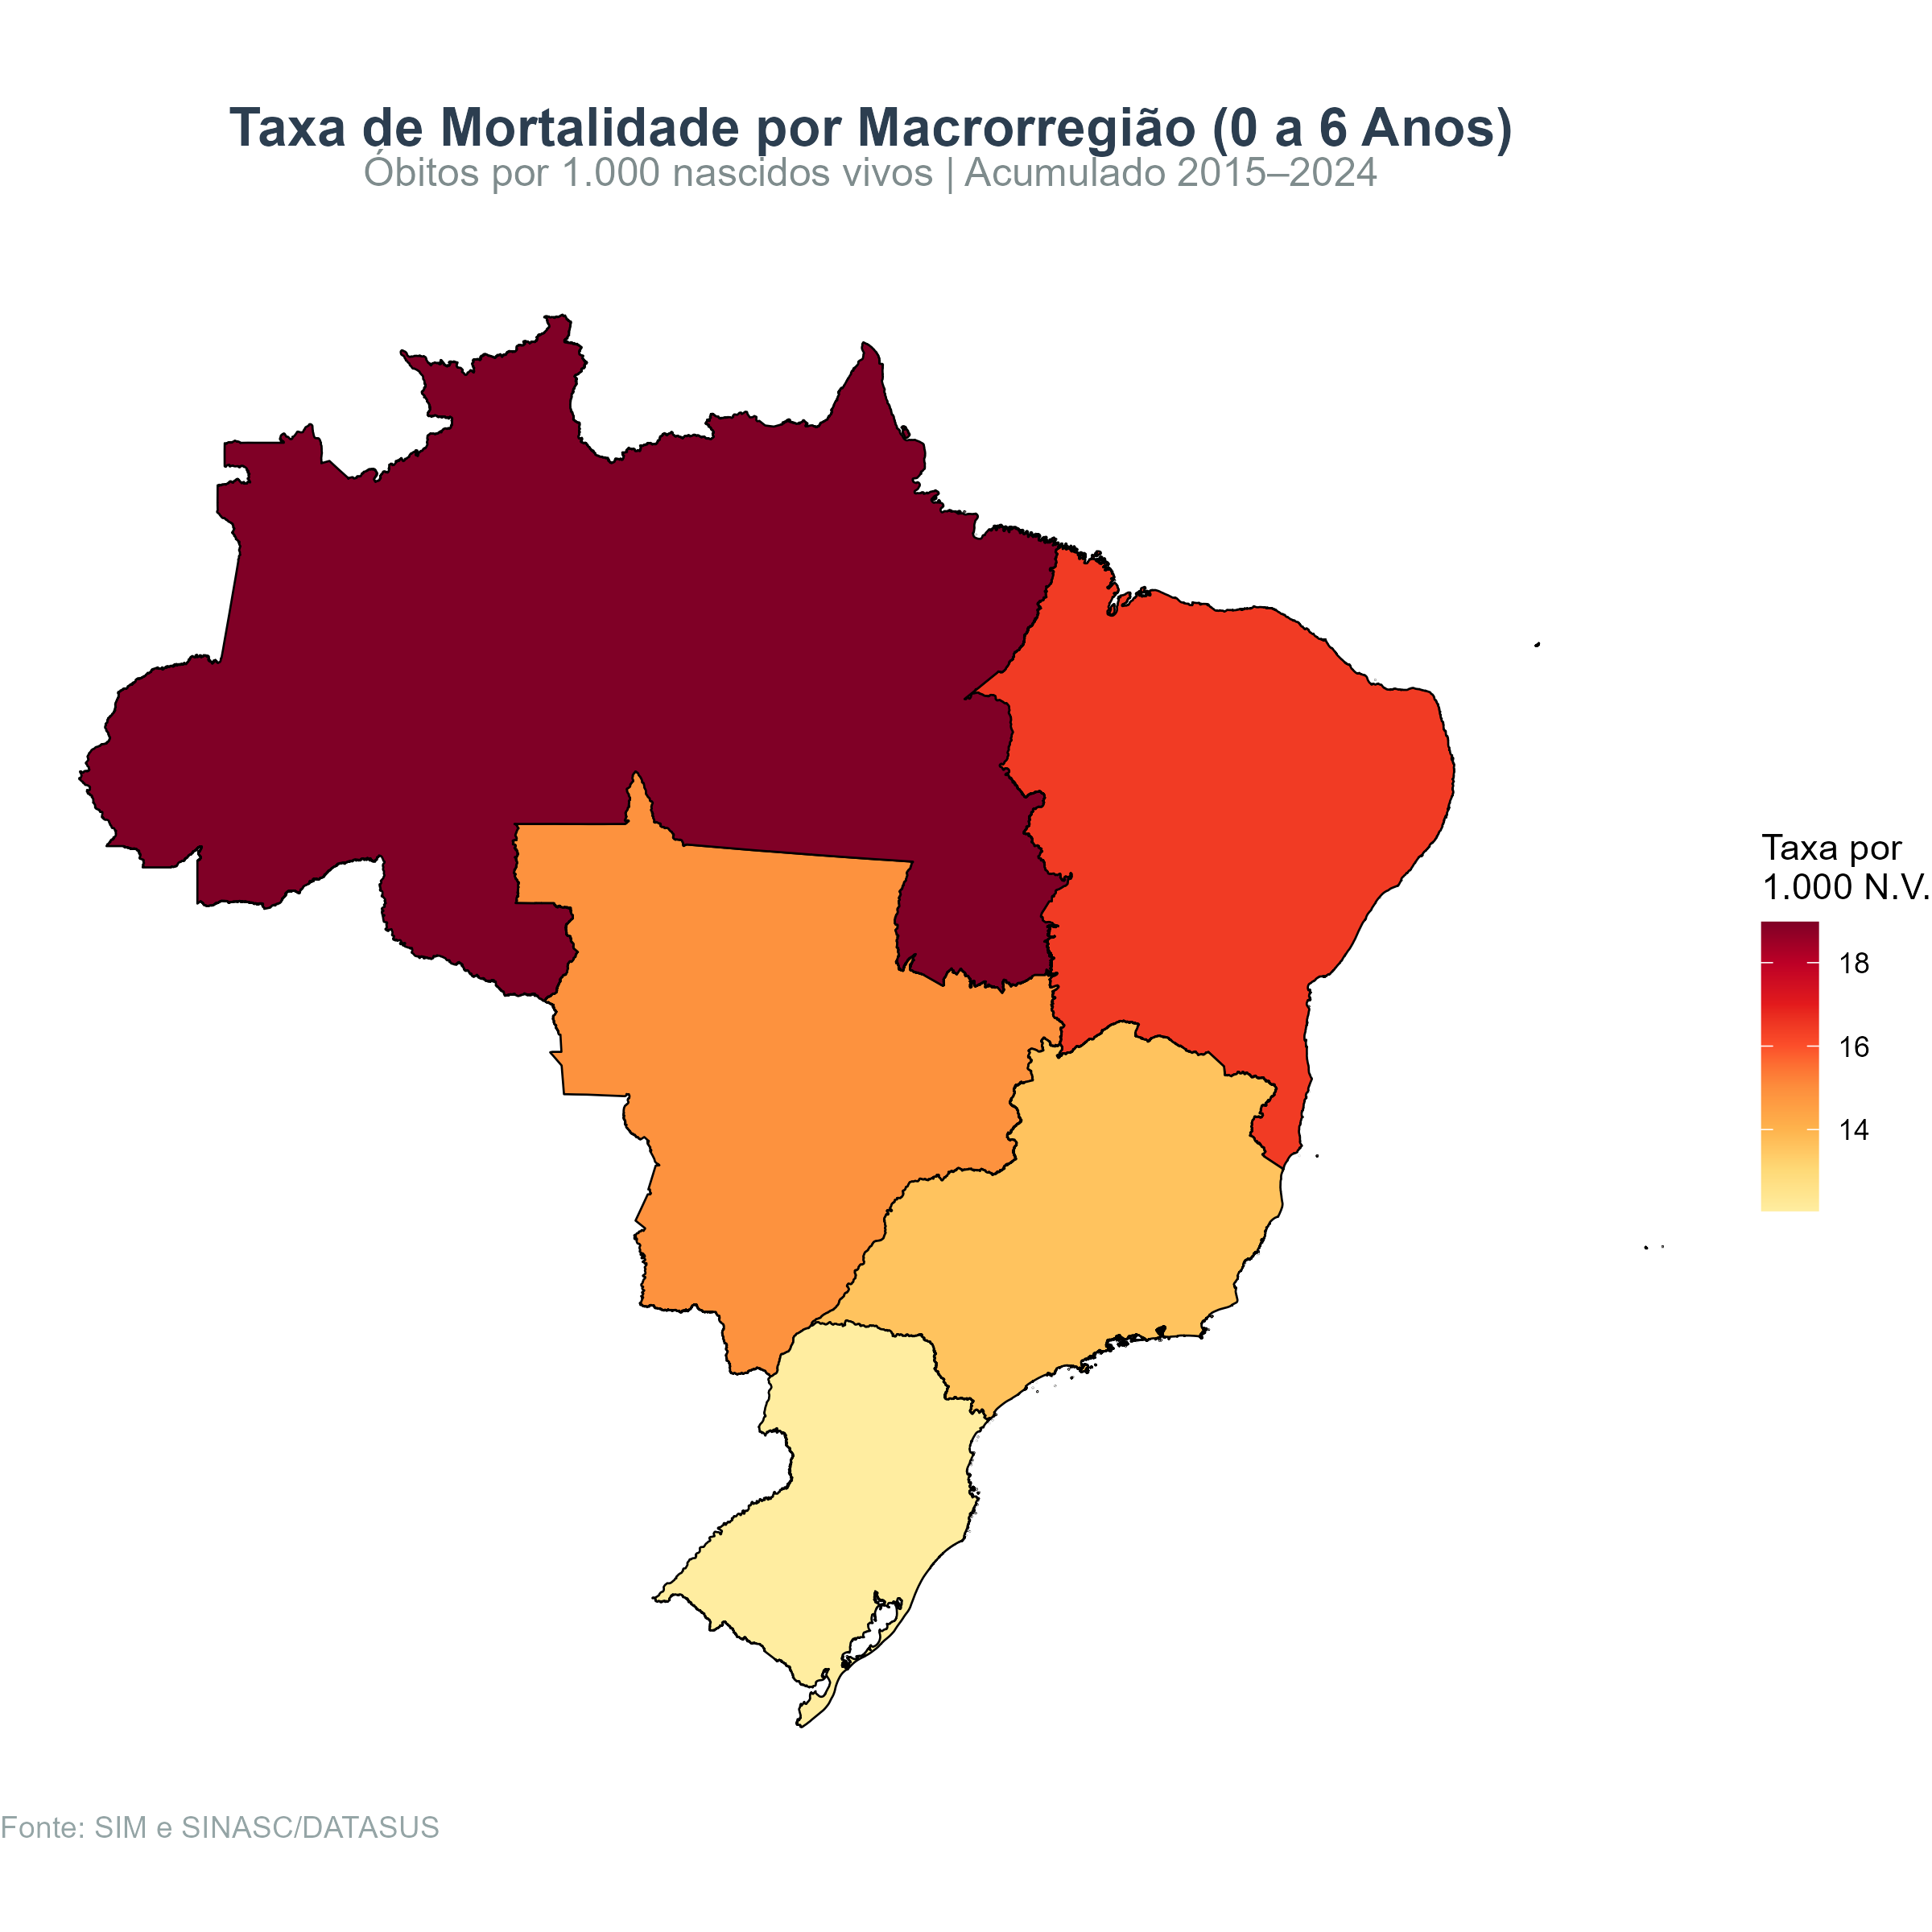
\includegraphics[width=0.6\linewidth,height=\textheight,keepaspectratio]{../outputs/SIM/Fig06_Mapa_Taxa_Macrorregiao.png}

}

\caption{Distribuição Espacial da Taxa de Mortalidade por Macrorregião,
2015-2024}

\end{figure}%
\end{frame}

\begin{frame}{Análise Espacial e Desigualdades Regionais da Mortalidade}
\protect\phantomsection\label{anuxe1lise-espacial-e-desigualdades-regionais-da-mortalidade-2}
\begin{figure}[H]

{\centering 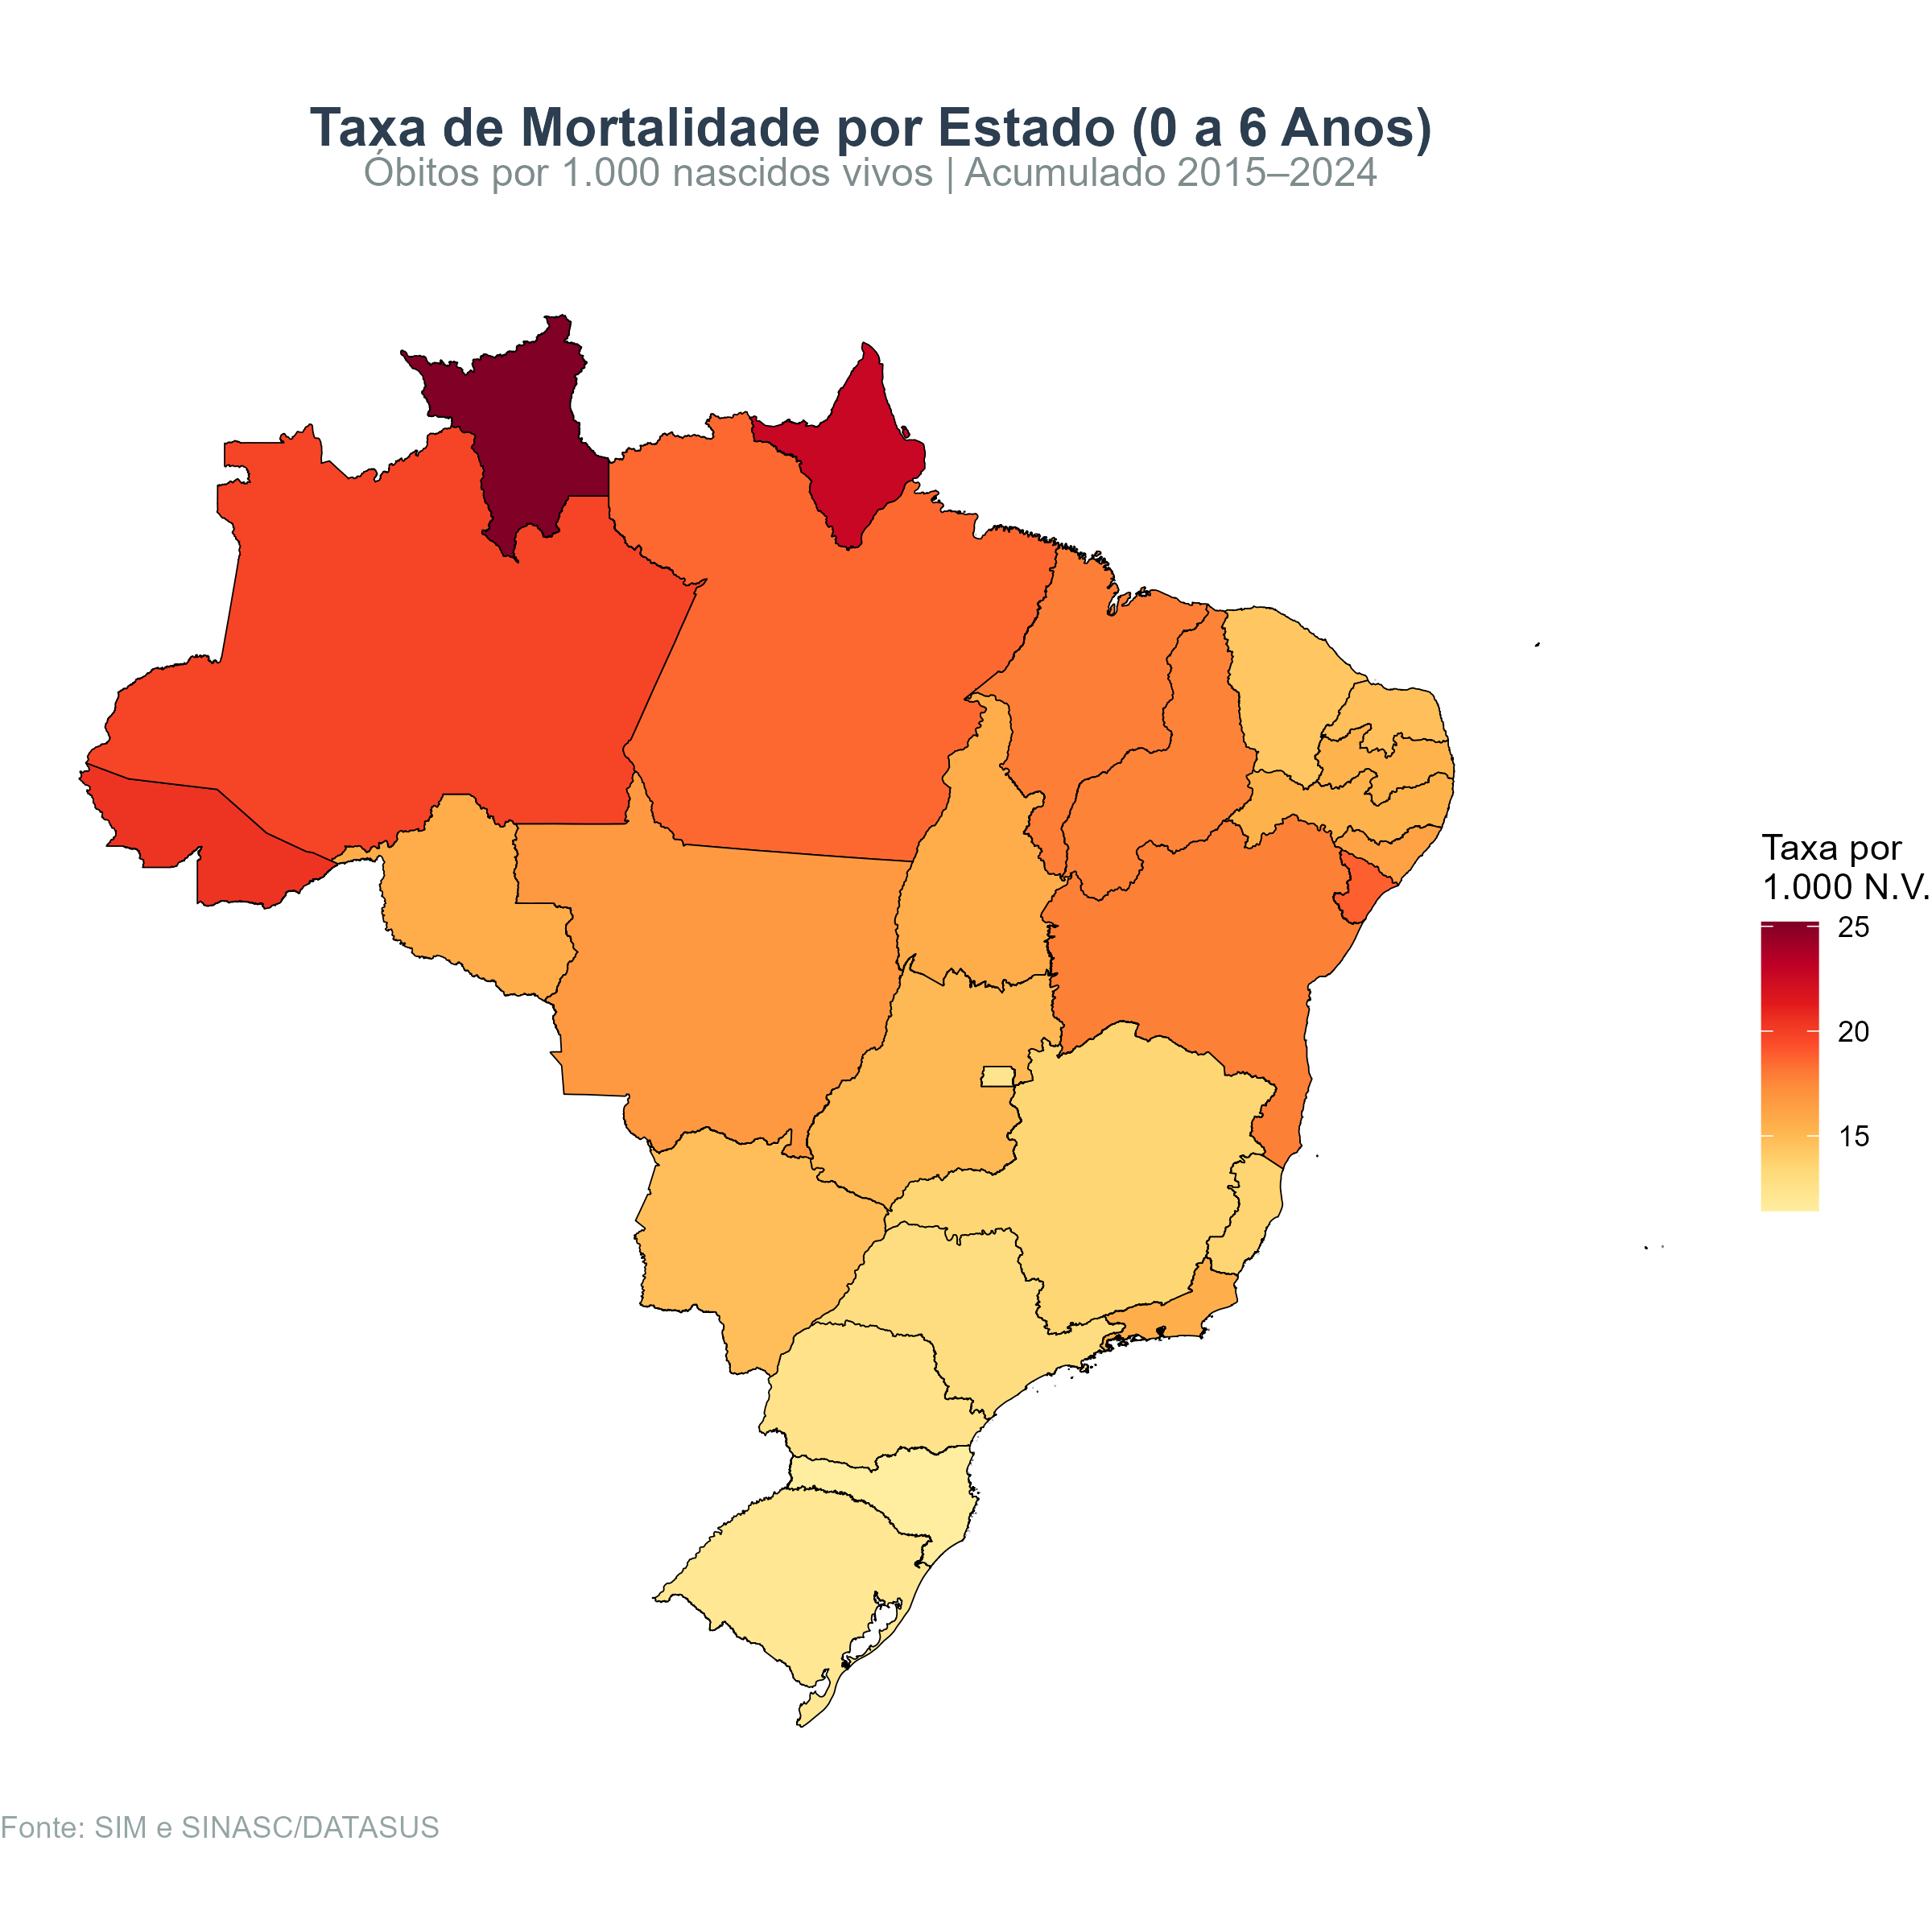
\includegraphics[width=0.6\linewidth,height=\textheight,keepaspectratio]{../outputs/SIM/Fig05_Mapa_Taxa_Estado.png}

}

\caption{Distribuição Espacial da Taxa de Mortalidade por Estado,
2015-2024}

\end{figure}%
\end{frame}

\begin{frame}{Fluxos de Mortalidade e Polos de Ocorrência}
\protect\phantomsection\label{fluxos-de-mortalidade-e-polos-de-ocorruxeancia}
\begin{itemize}
\tightlist
\item
  A análise de fluxo cruza o \textbf{município de residência} da criança
  com o \textbf{município de ocorrência do óbito}, permitindo
  identificar deslocamentos assistenciais, dependência regional e
  concentração de óbitos em polos de saúde infantil.
\end{itemize}
\end{frame}

\begin{frame}{Fluxos de Mortalidade e Polos de Ocorrência}
\protect\phantomsection\label{fluxos-de-mortalidade-e-polos-de-ocorruxeancia-1}
\begin{figure}[H]

{\centering 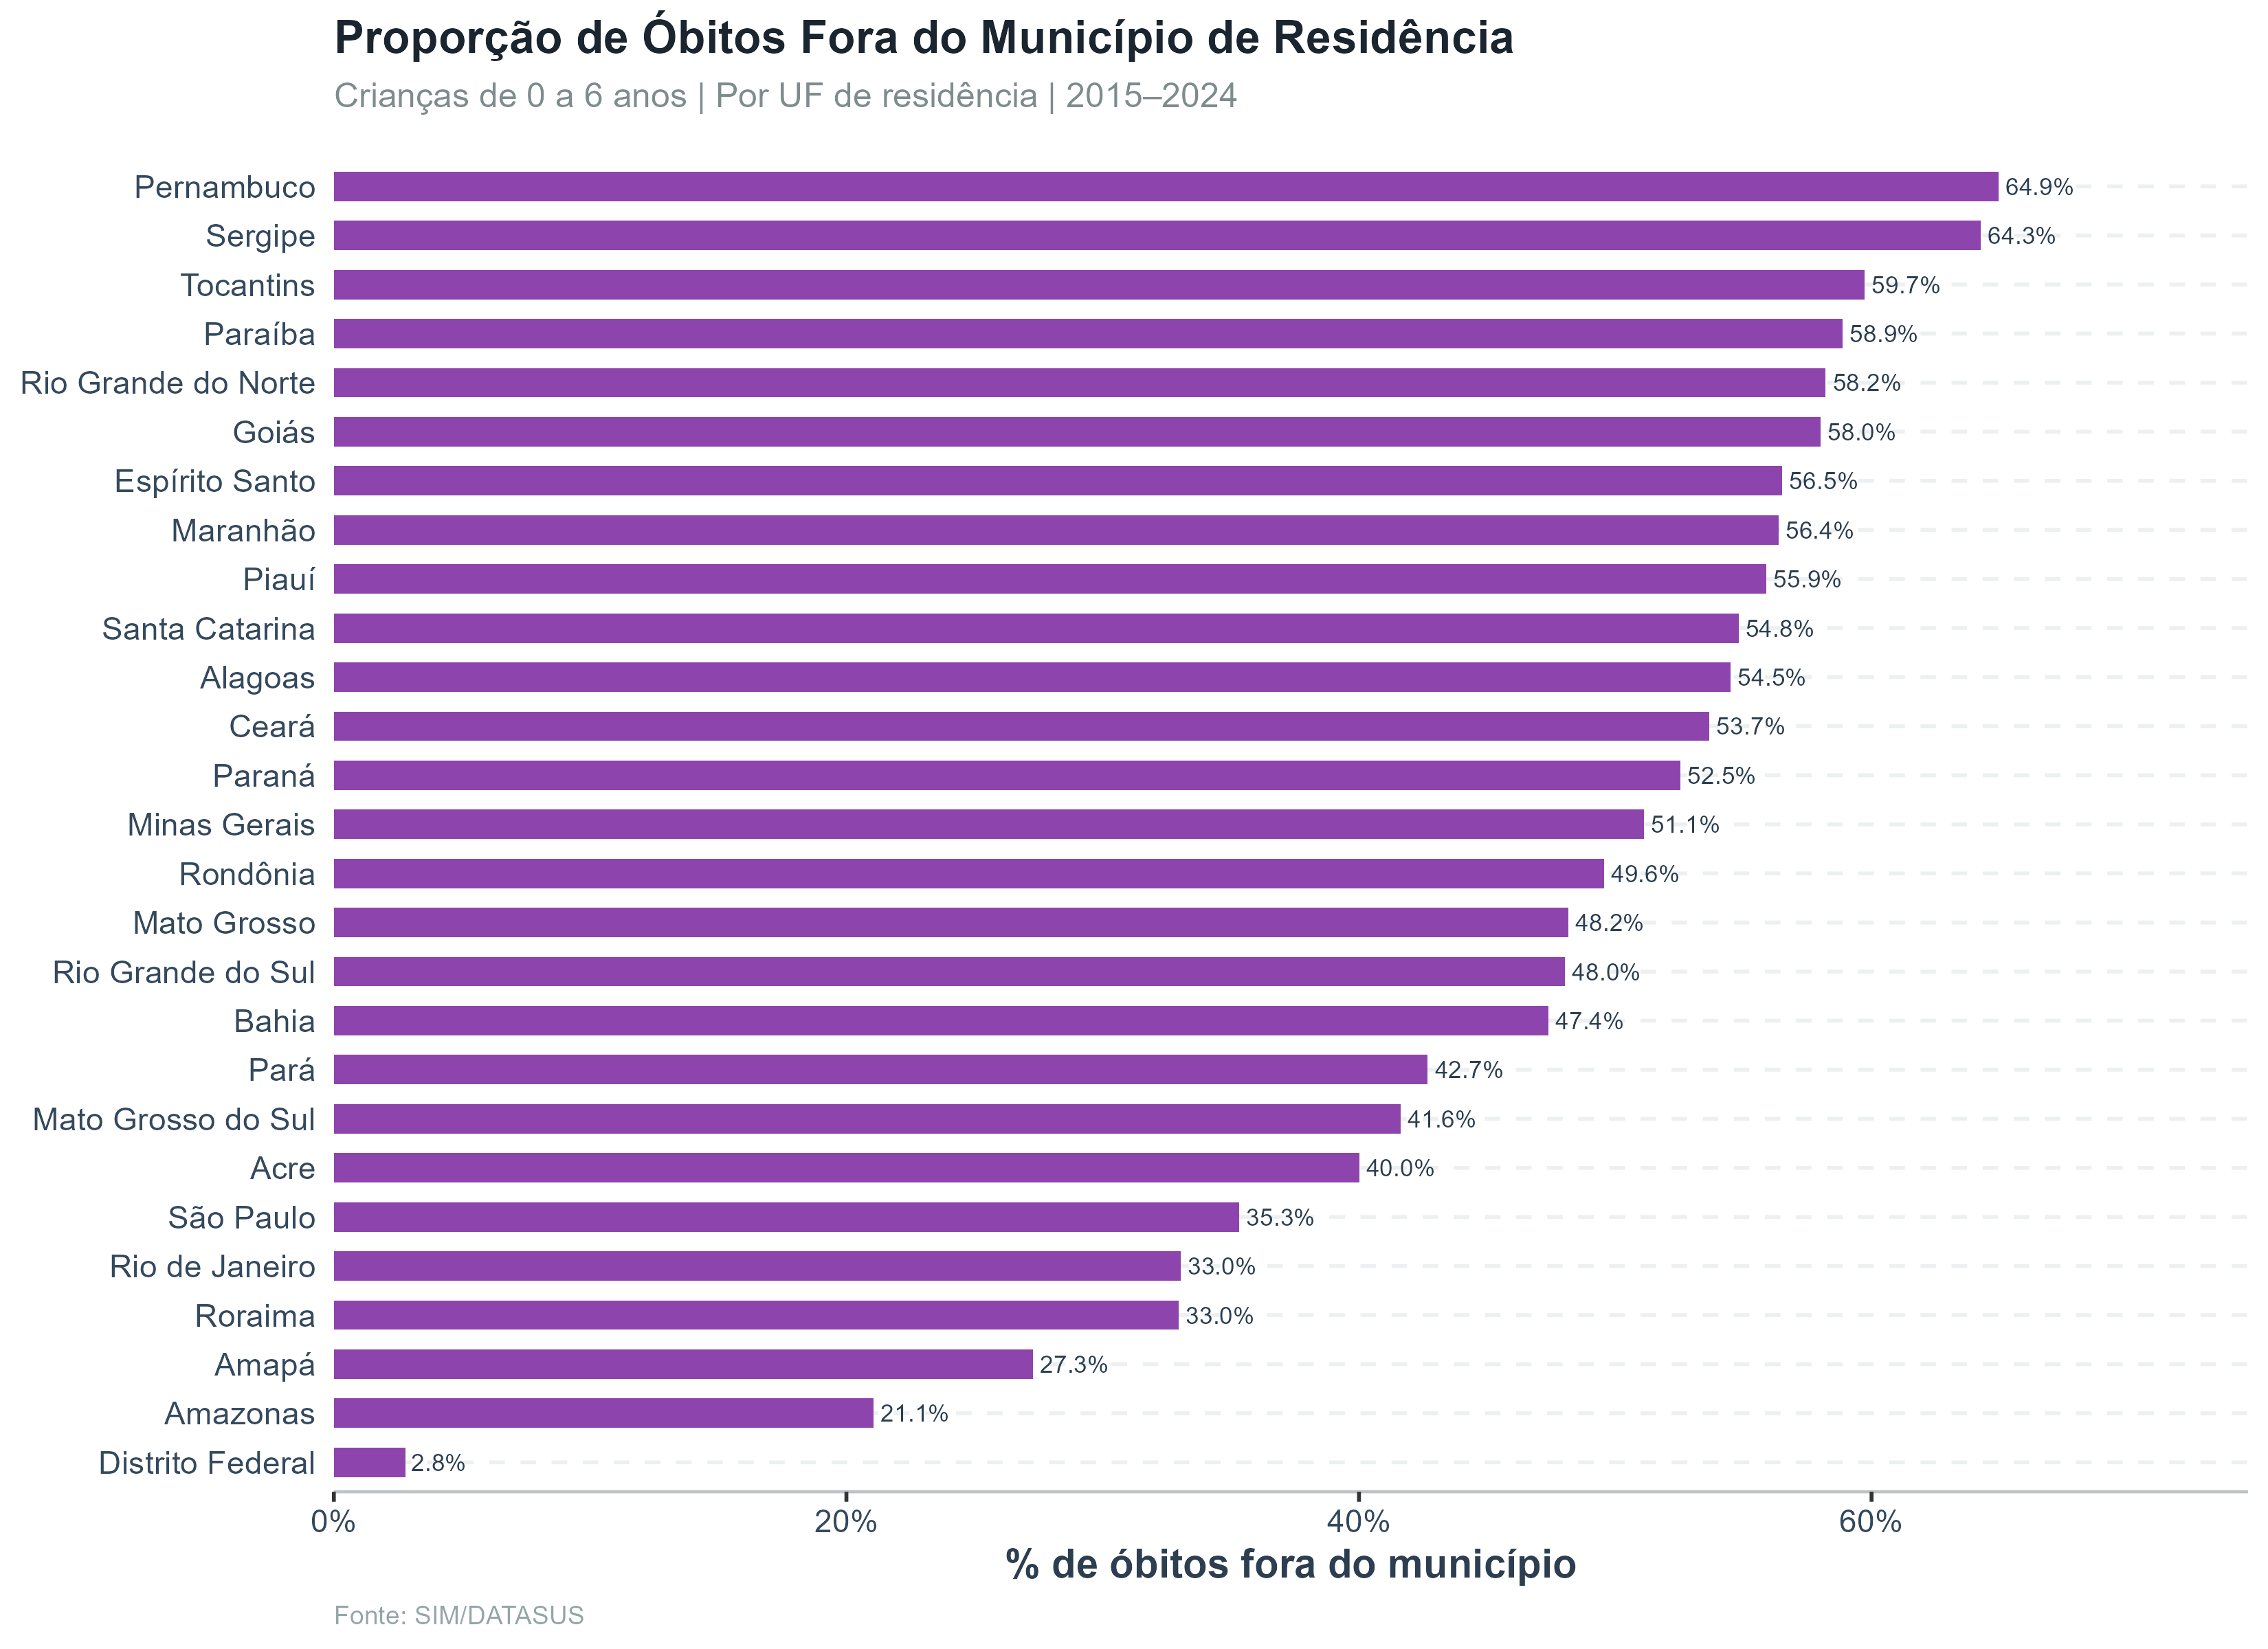
\includegraphics[width=0.9\linewidth,height=\textheight,keepaspectratio]{../outputs/SIM/Fig07_Fluxo_Obitos_Fora_Municipio.png}

}

\caption{Proporção de Óbitos Fora do Município de Residência, 2015-2024}

\end{figure}%
\end{frame}

\begin{frame}{Fluxos de Mortalidade e Polos de Ocorrência}
\protect\phantomsection\label{fluxos-de-mortalidade-e-polos-de-ocorruxeancia-2}
\begin{figure}[H]

{\centering 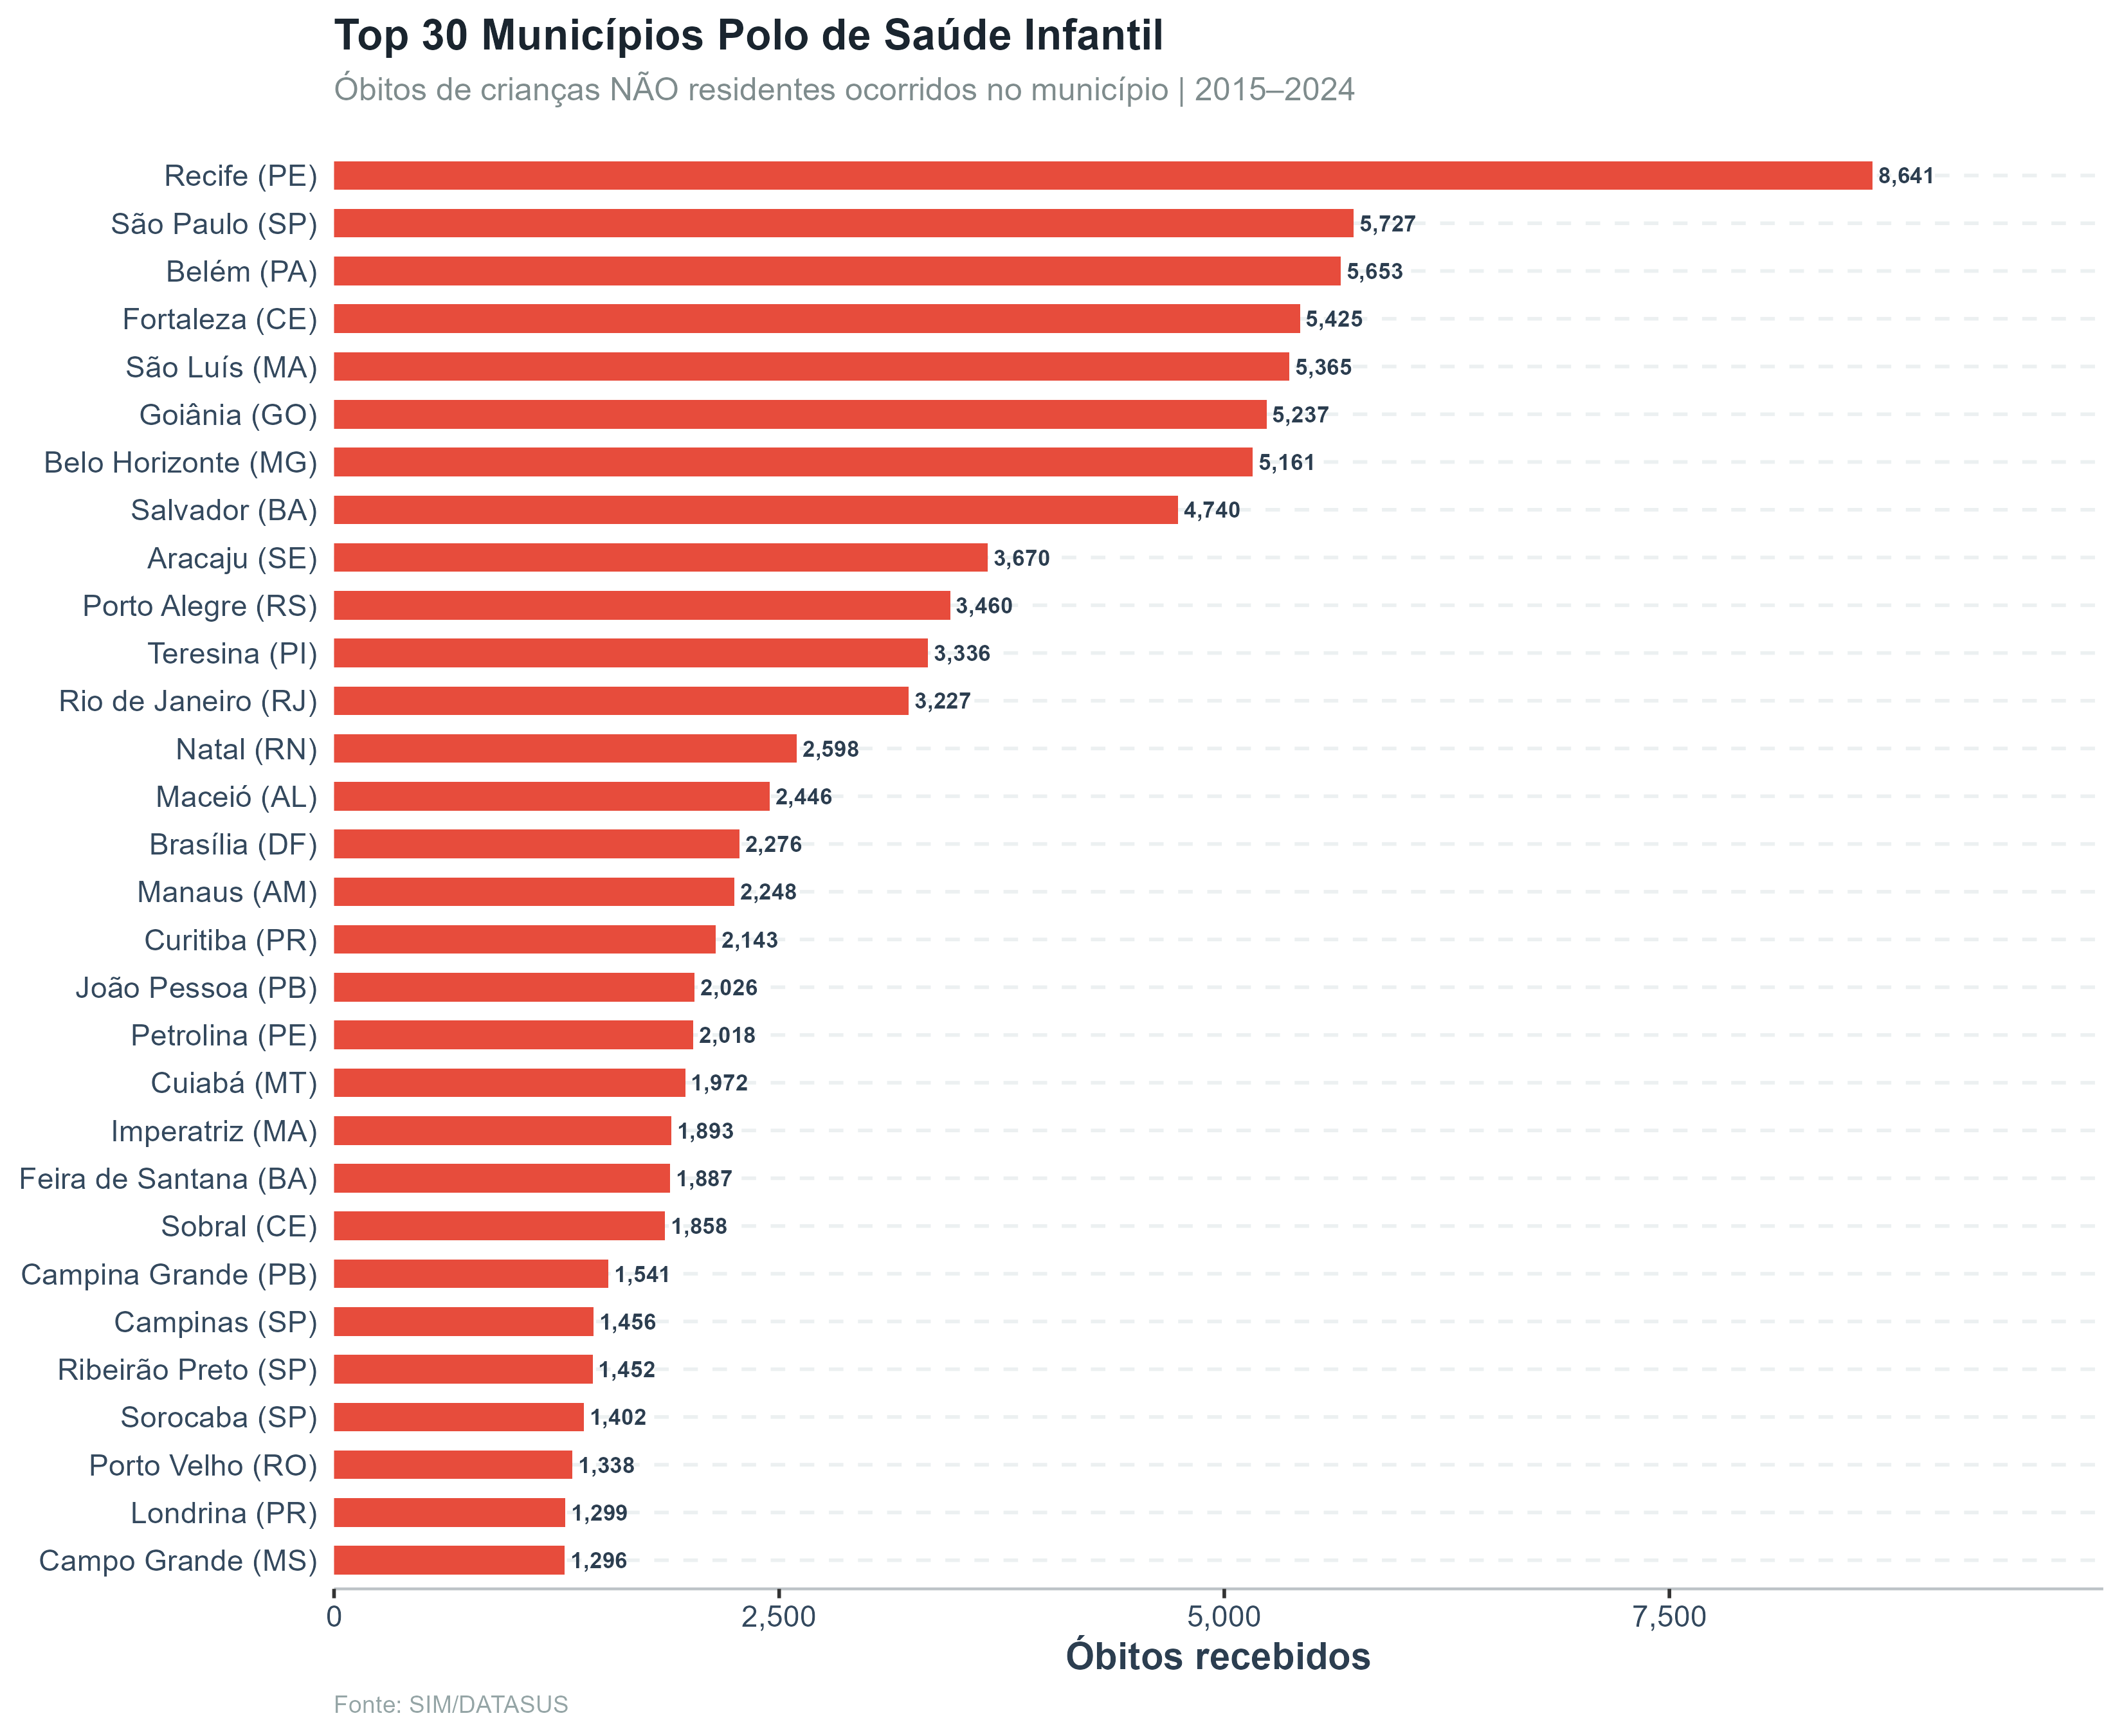
\includegraphics[width=0.8\linewidth,height=\textheight,keepaspectratio]{../outputs/SIM/Fig08_Polos_Saude_Infantil_Top30.png}

}

\caption{Municípios Polo de Saúde Infantil, 2015-2024}

\end{figure}%
\end{frame}

\begin{frame}{Fluxos de Mortalidade e Polos de Ocorrência}
\protect\phantomsection\label{fluxos-de-mortalidade-e-polos-de-ocorruxeancia-3}
\begin{figure}[H]

{\centering 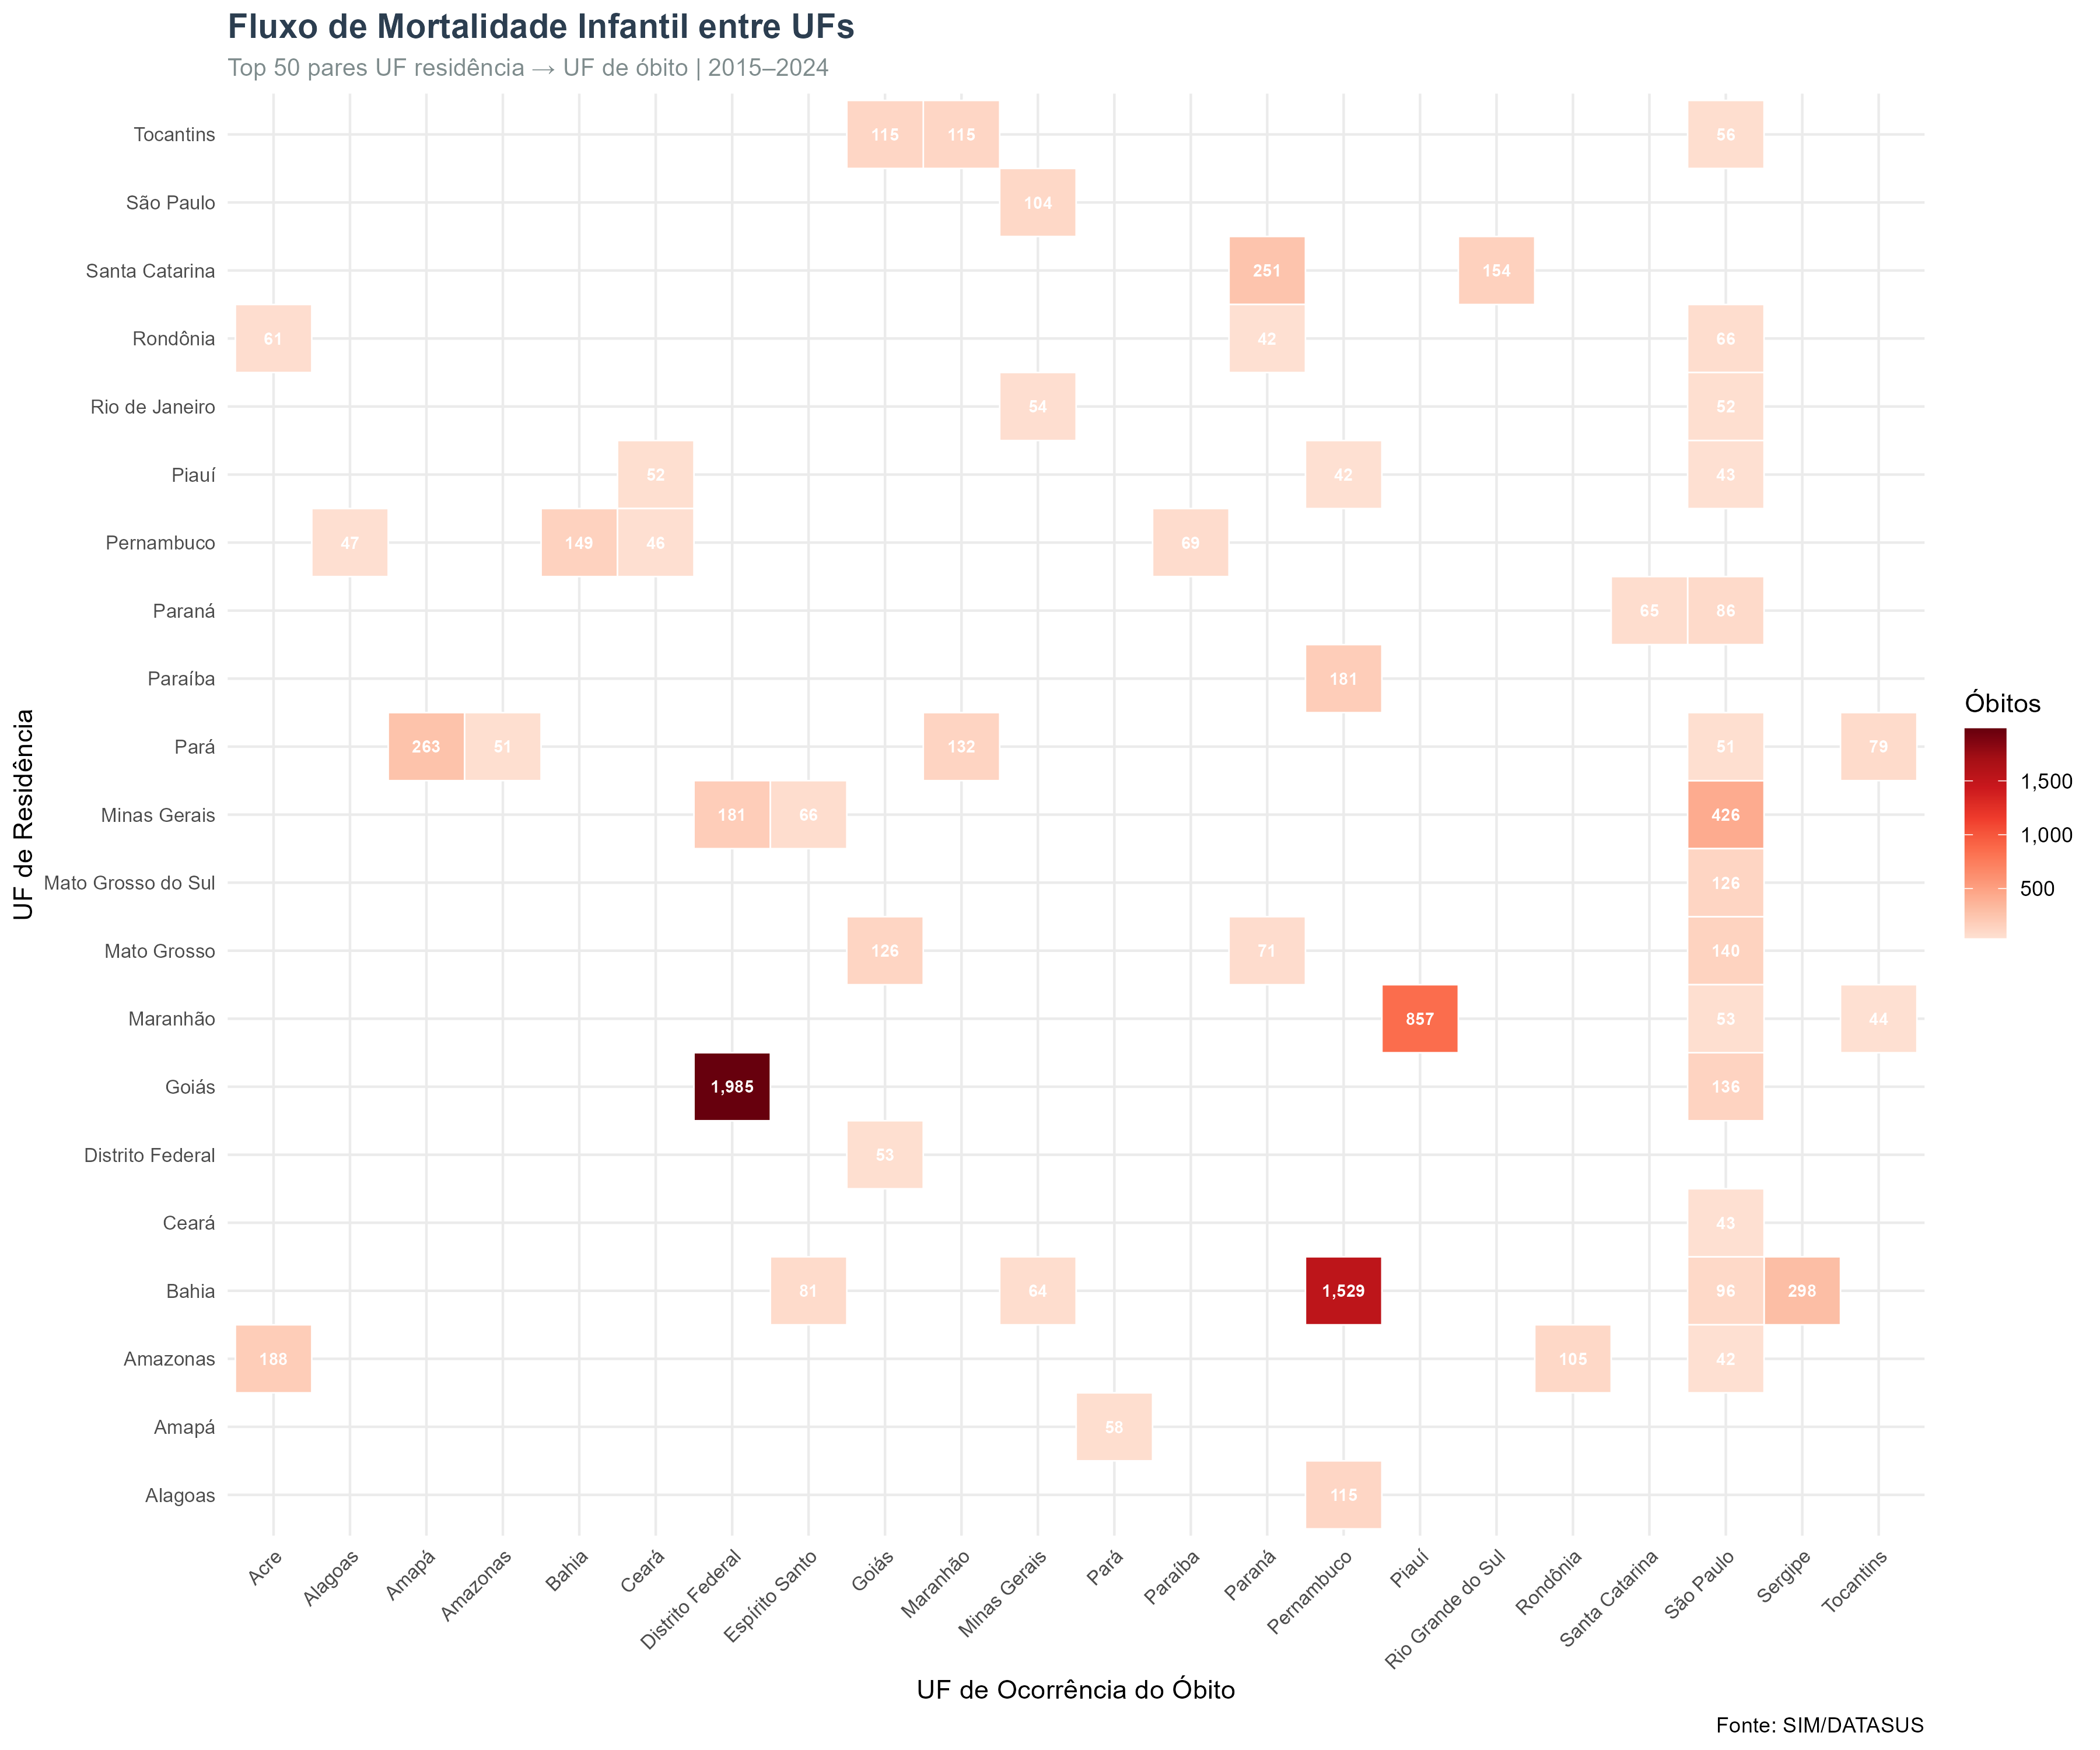
\includegraphics[width=0.75\linewidth,height=\textheight,keepaspectratio]{../outputs/SIM/Fig09_Heatmap_Fluxo_InterUF.png}

}

\caption{Fluxo de Mortalidade Infantil entre Estados, 2015-2024}

\end{figure}%
\end{frame}

\begin{frame}{Fluxos de Mortalidade e Polos de Ocorrência}
\protect\phantomsection\label{fluxos-de-mortalidade-e-polos-de-ocorruxeancia-4}
\begin{figure}[H]

{\centering 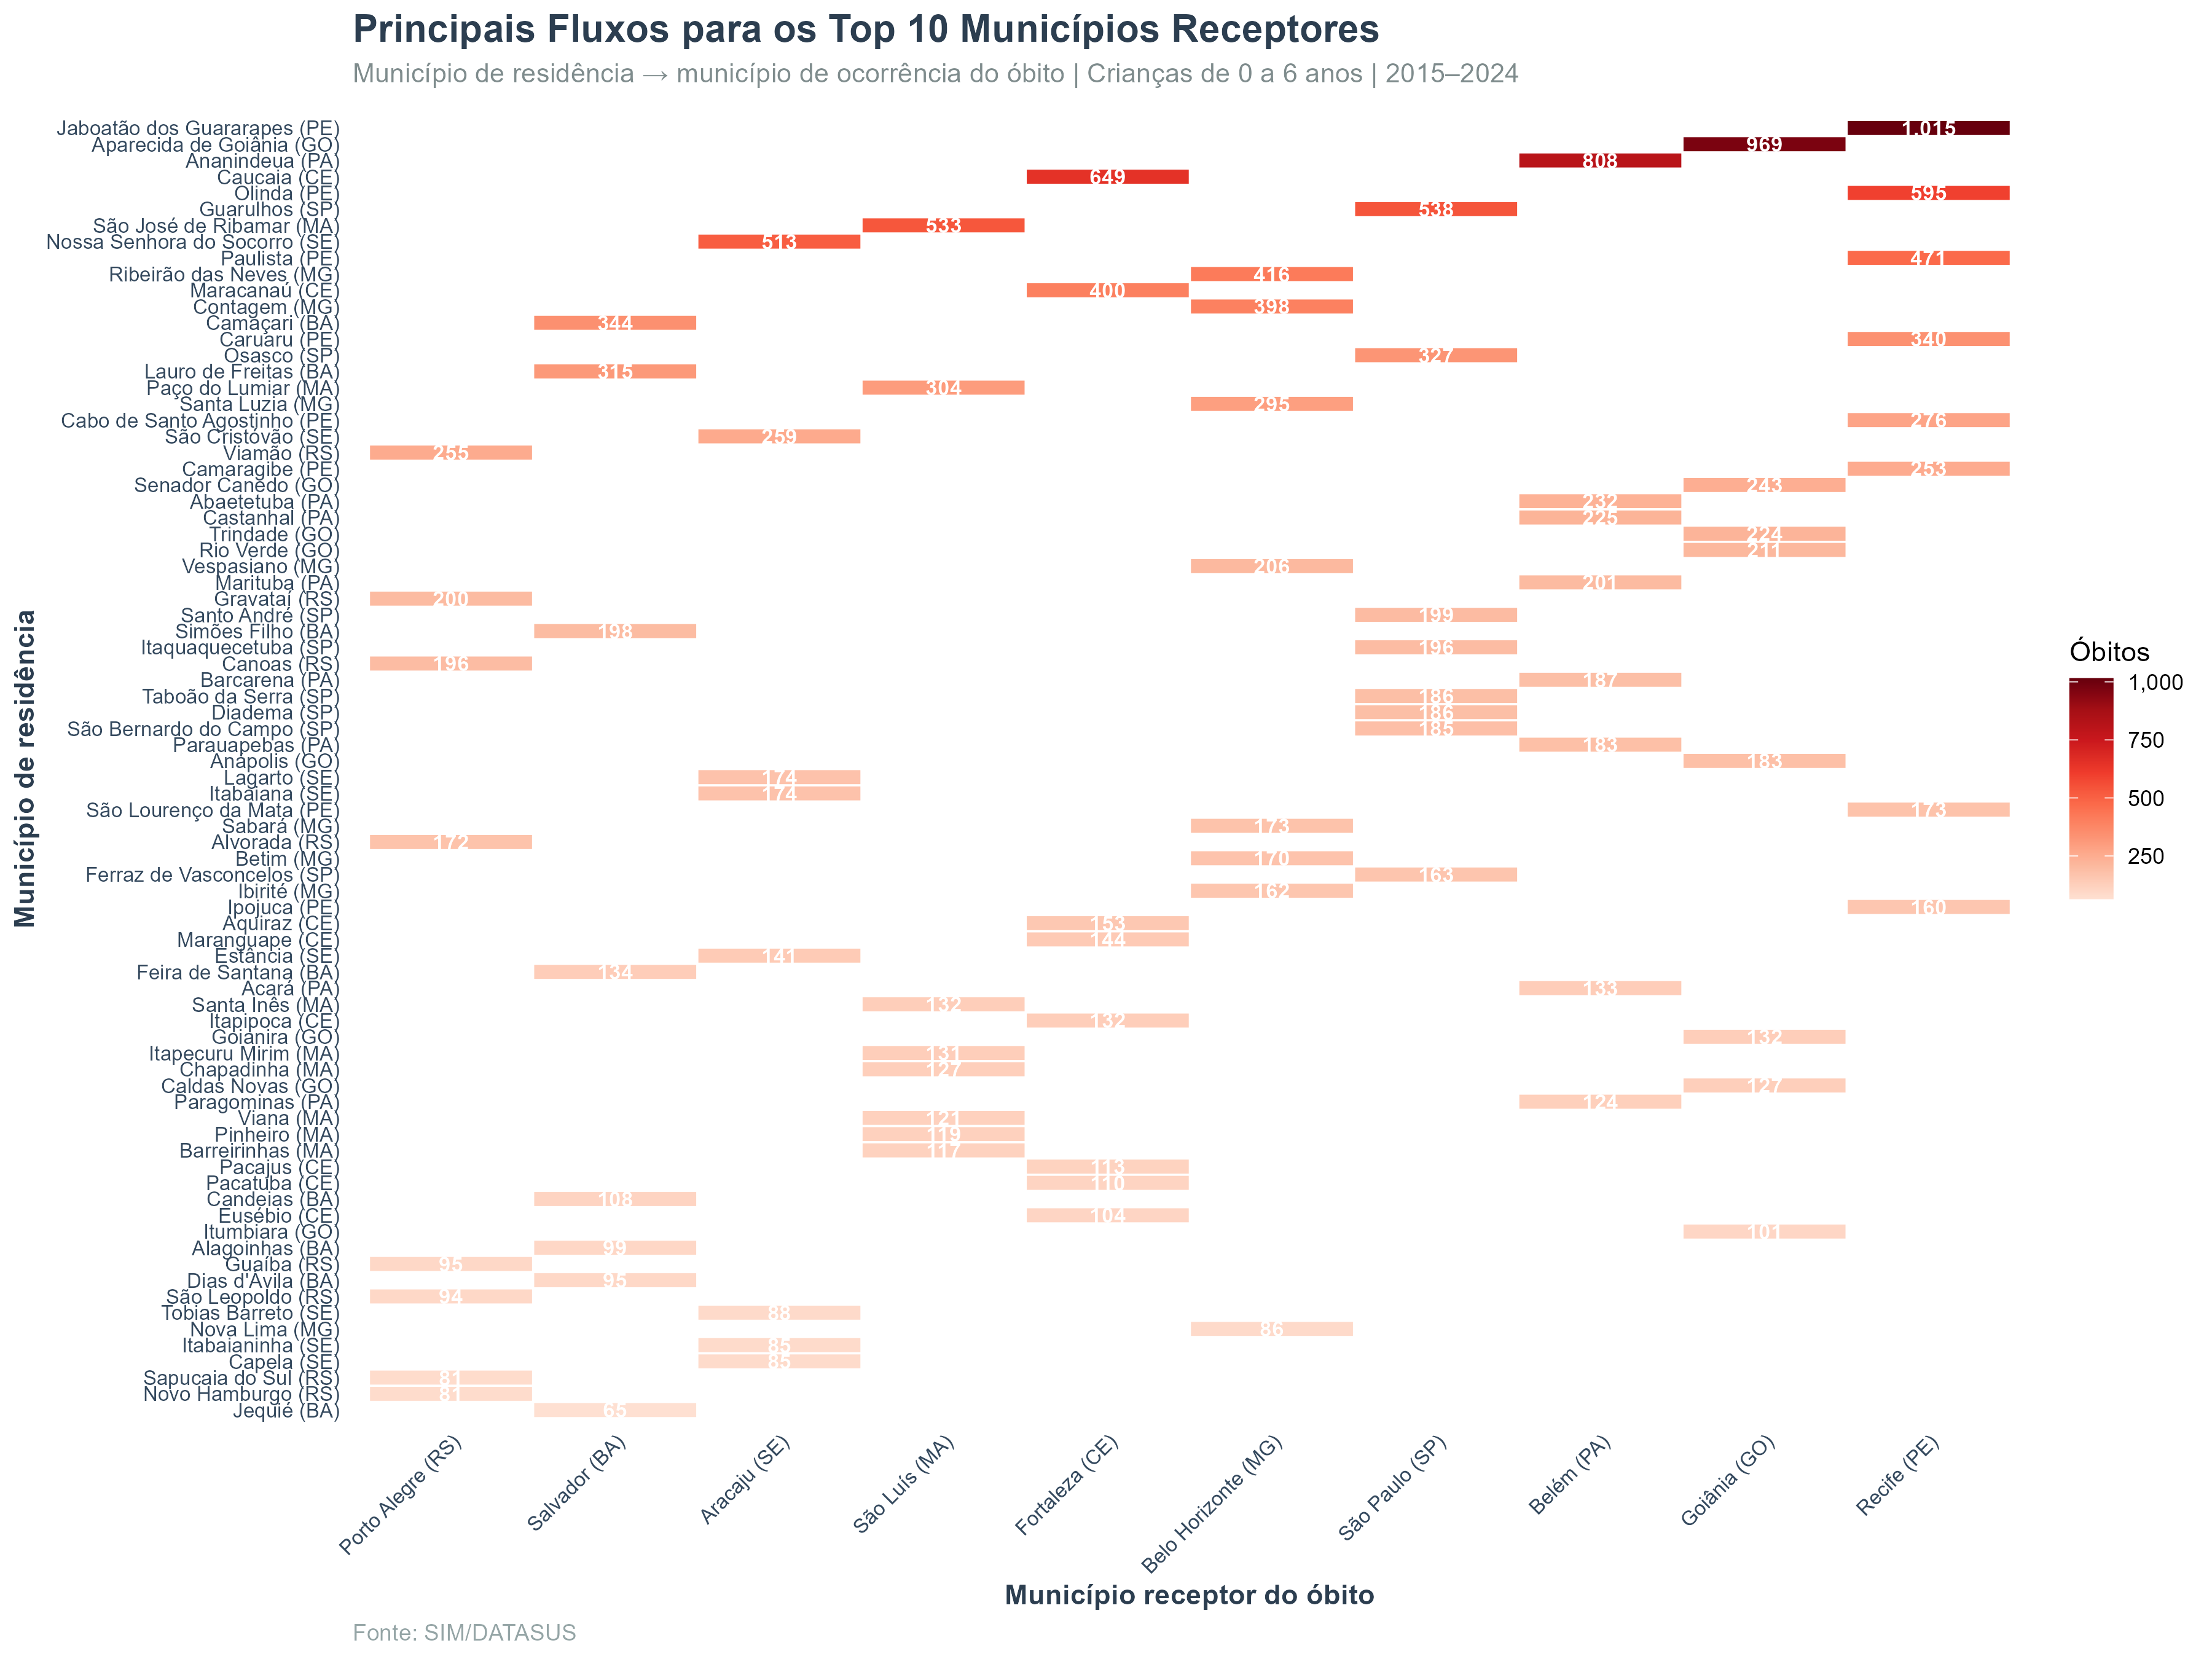
\includegraphics[width=0.8\linewidth,height=\textheight,keepaspectratio]{../outputs/SIM/Fig10_Fluxos_Top10_Municipios_Receptores.png}

}

\caption{Principais Fluxos para Municípios Mais Receptores de Óbitos,
2015-2024}

\end{figure}%
\end{frame}

\begin{frame}{Segmentação Diagnóstica e Polos de Referência}
\protect\phantomsection\label{segmentauxe7uxe3o-diagnuxf3stica-e-polos-de-referuxeancia}
\begin{itemize}
\item
  As causas são segmentadas em grupos diagnósticos de \textbf{alta
  complexidade} e cruzadas com as faixas etárias e com a origem dos
  pacientes em nível de \textbf{município}.\\
\item
  As afecções perinatais aparecem destacadas dos demais grupos, e o
  fluxo de \textbf{referência terapêutica} (alta complexidade sem
  perinatal) é usado para revelar a vocação de cada polo e os
  deslocamentos efetivos por tratamento.
\end{itemize}
\end{frame}

\begin{frame}{Segmentação Diagnóstica nos Polos}
\protect\phantomsection\label{segmentauxe7uxe3o-diagnuxf3stica-nos-polos}
\begin{figure}[H]

{\centering 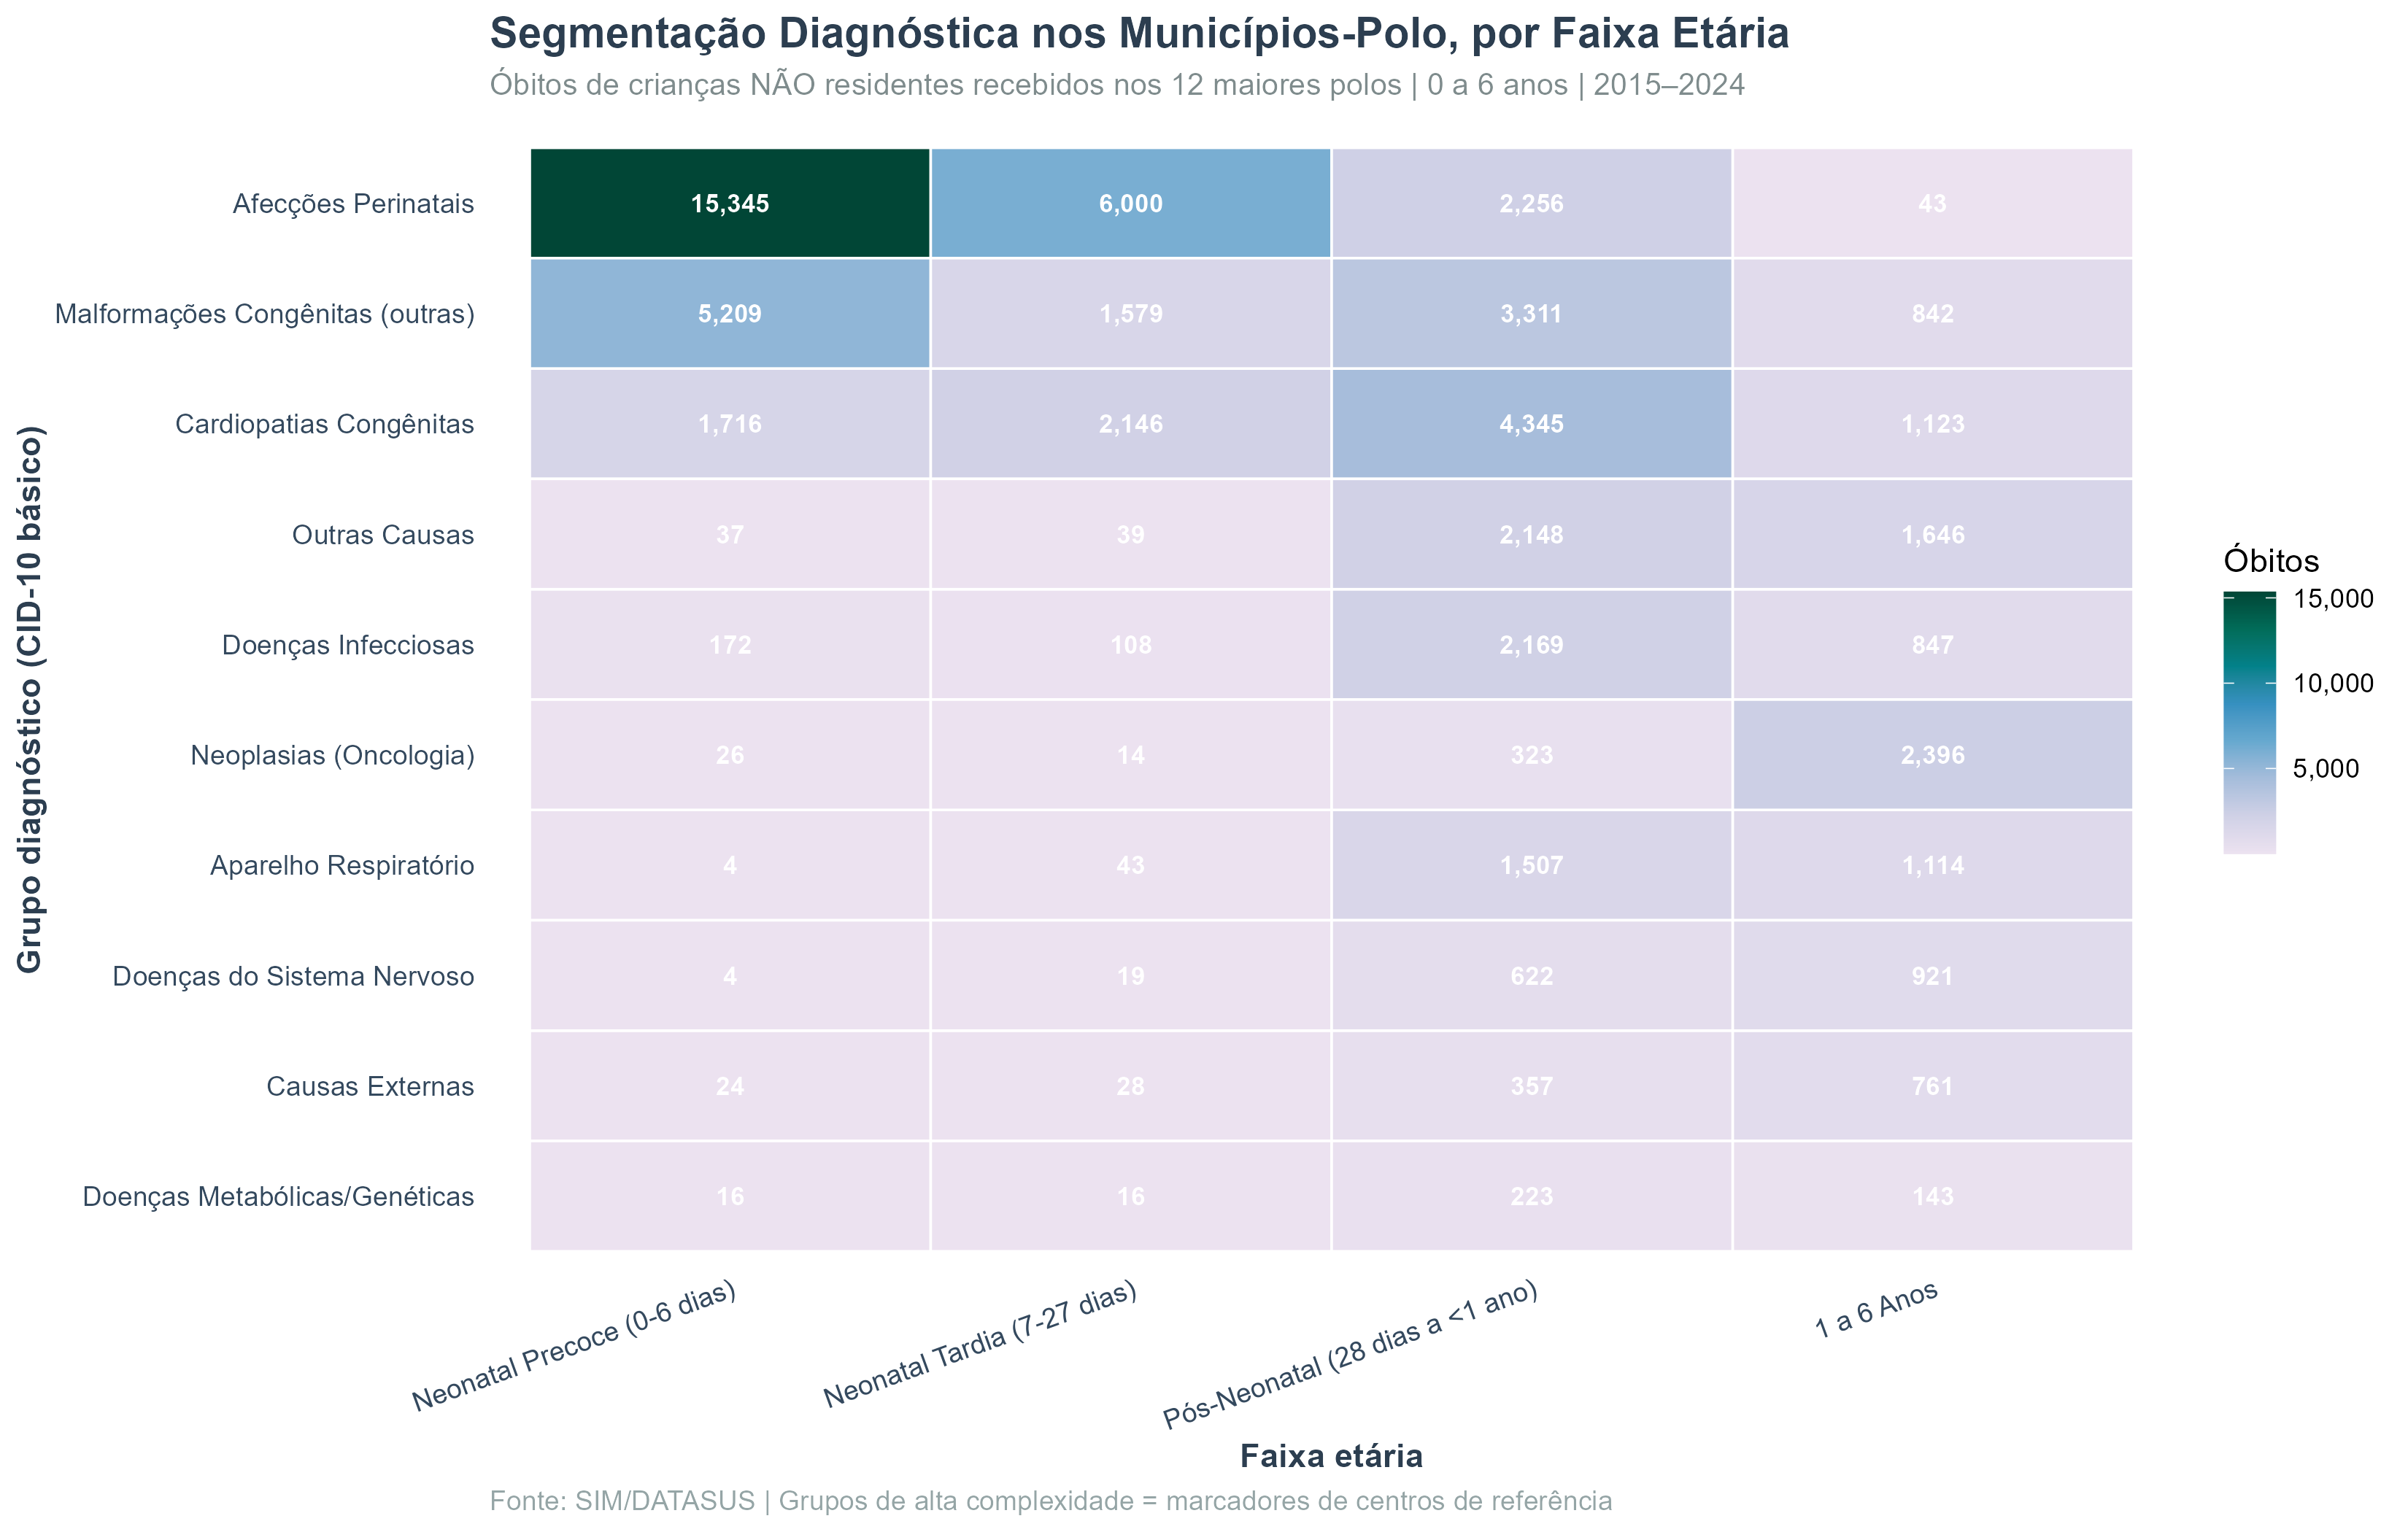
\includegraphics[width=0.9\linewidth,height=\textheight,keepaspectratio]{../outputs/SIM/Fig11_CID_Segmentado_por_Faixa_Polos.png}

}

\caption{Segmentação Diagnóstica nos Polos, por Faixa Etária, 2015-2024}

\end{figure}%
\end{frame}

\begin{frame}{Polos por Especialidade}
\protect\phantomsection\label{polos-por-especialidade}
\begin{figure}[H]

{\centering 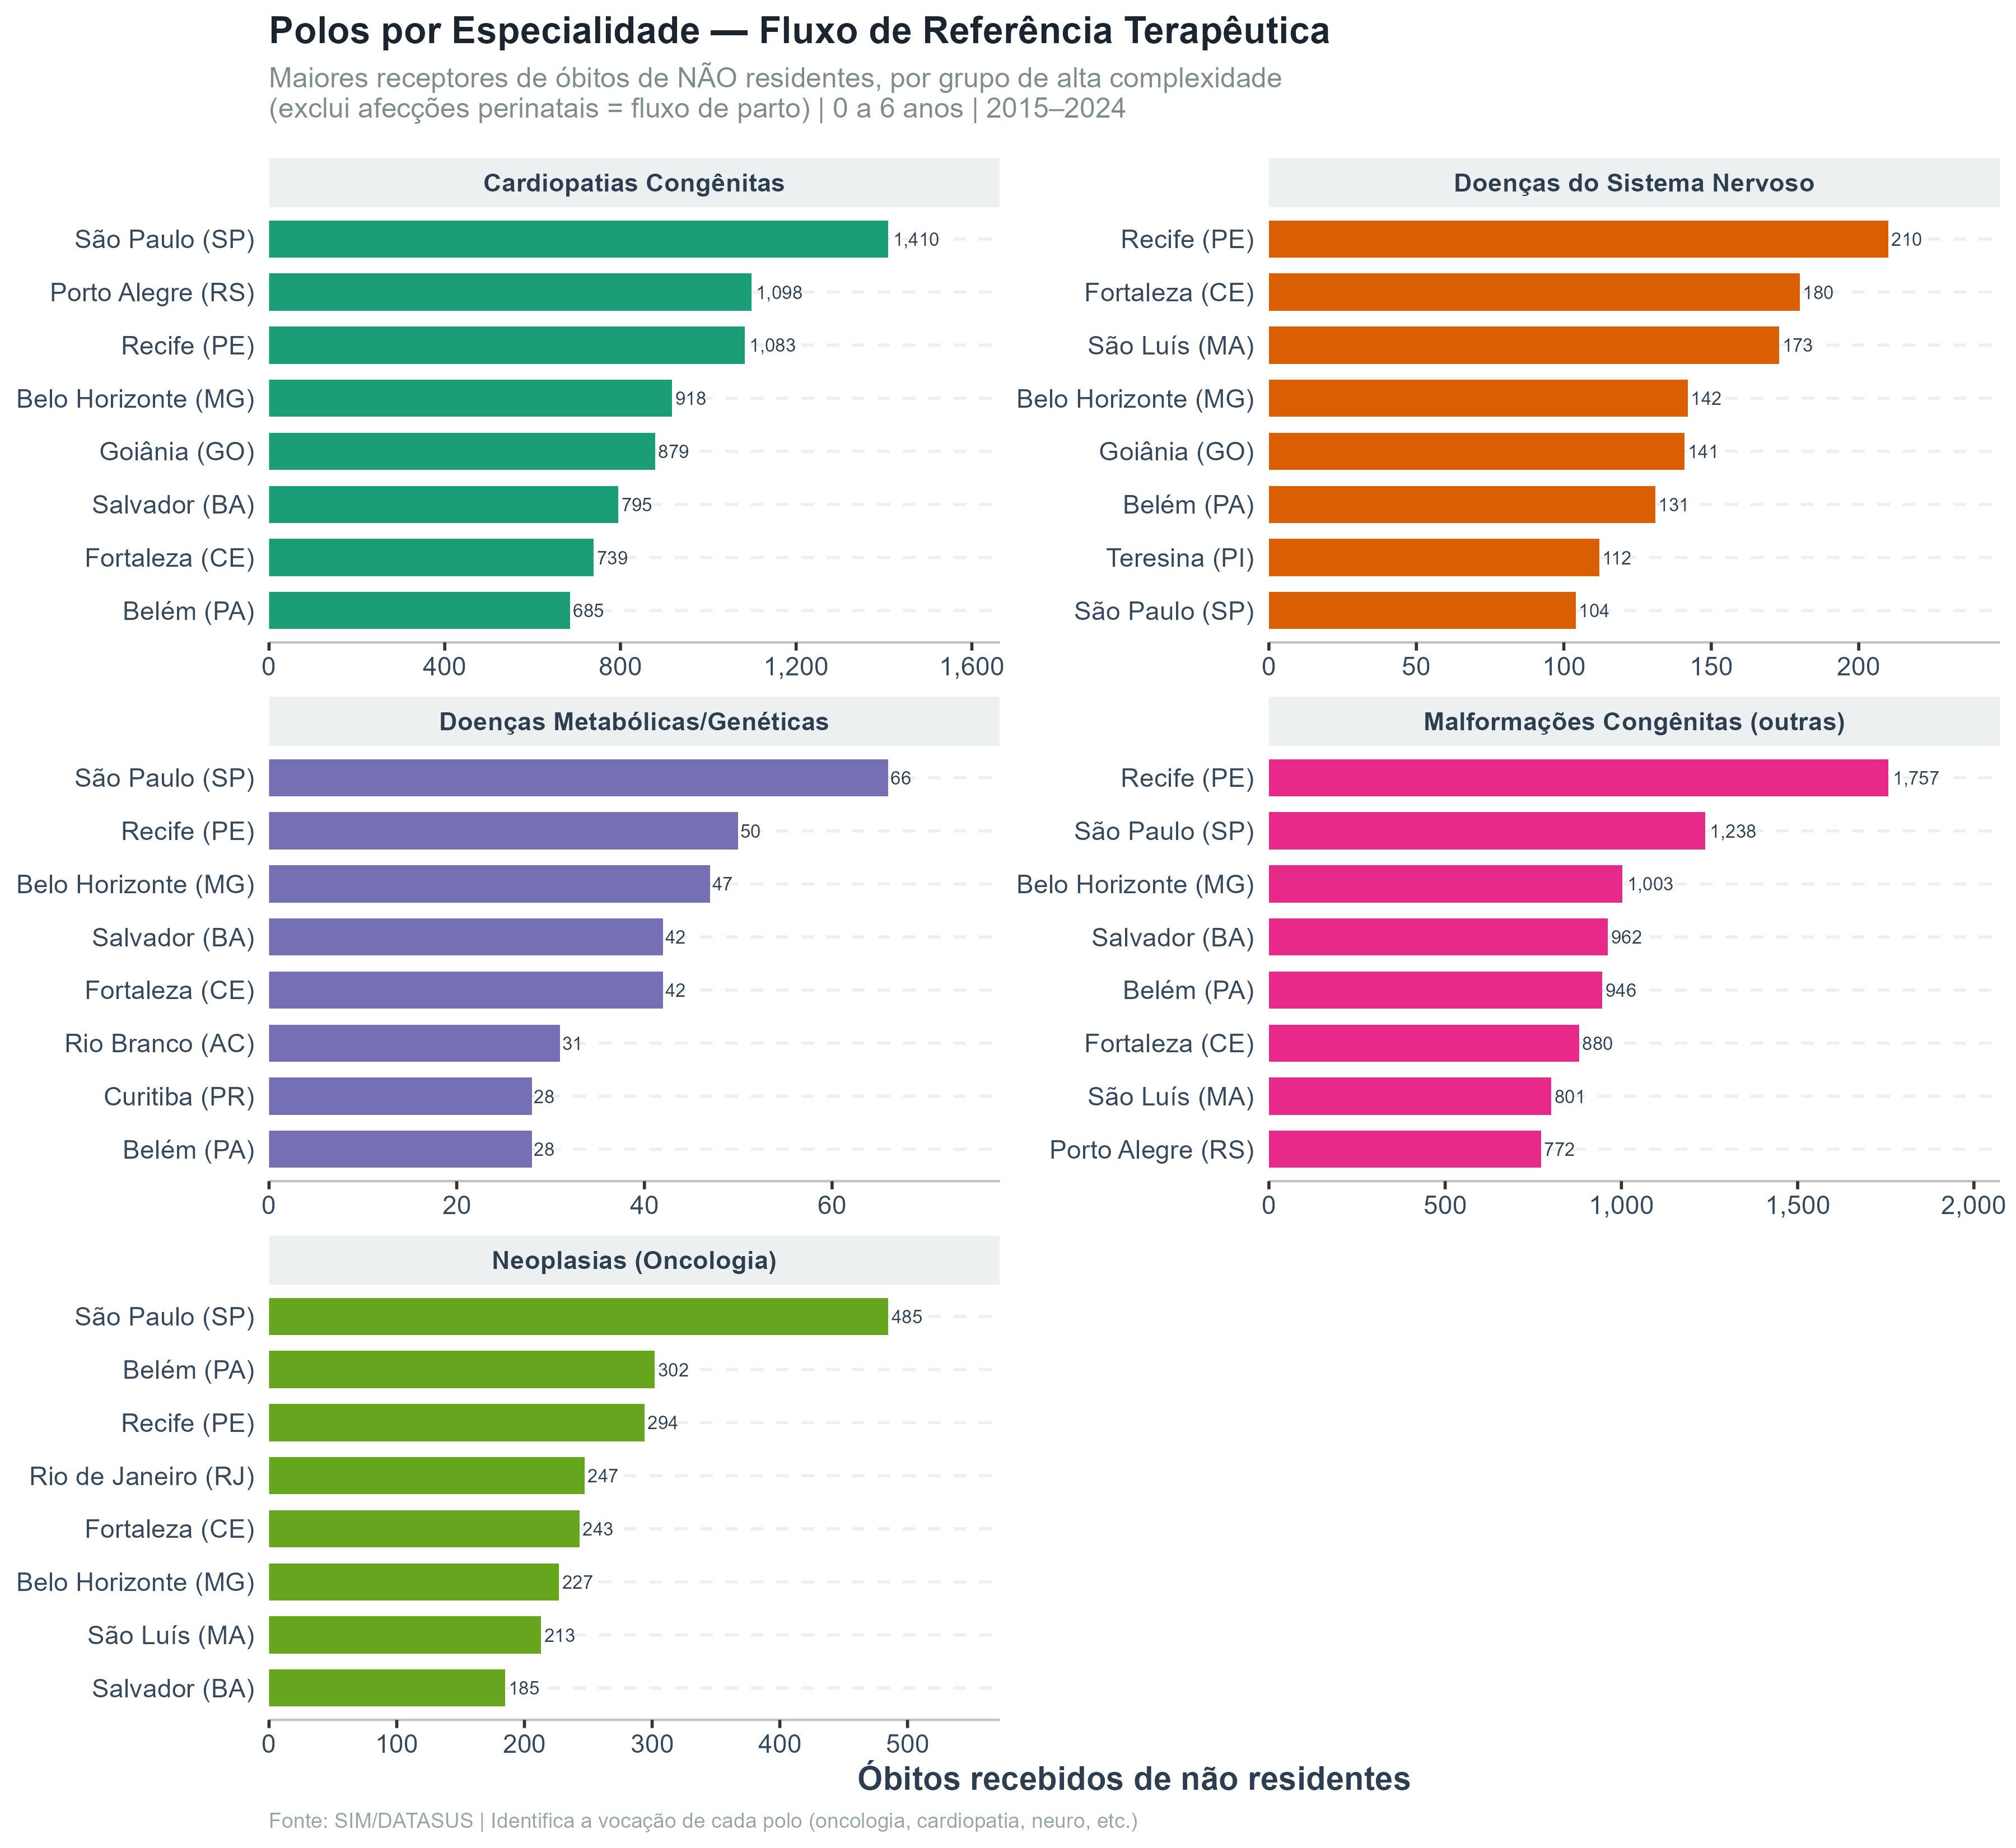
\includegraphics[width=0.6\linewidth,height=\textheight,keepaspectratio]{../outputs/SIM/Fig13_Polos_por_Especialidade.png}

}

\caption{Polos por Especialidade --- Fluxo de Referência Terapêutica,
2015-2024}

\end{figure}%
\end{frame}

\begin{frame}{Fluxo Origem ao Polo}
\protect\phantomsection\label{fluxo-origem-ao-polo}
\begin{figure}[H]

{\centering 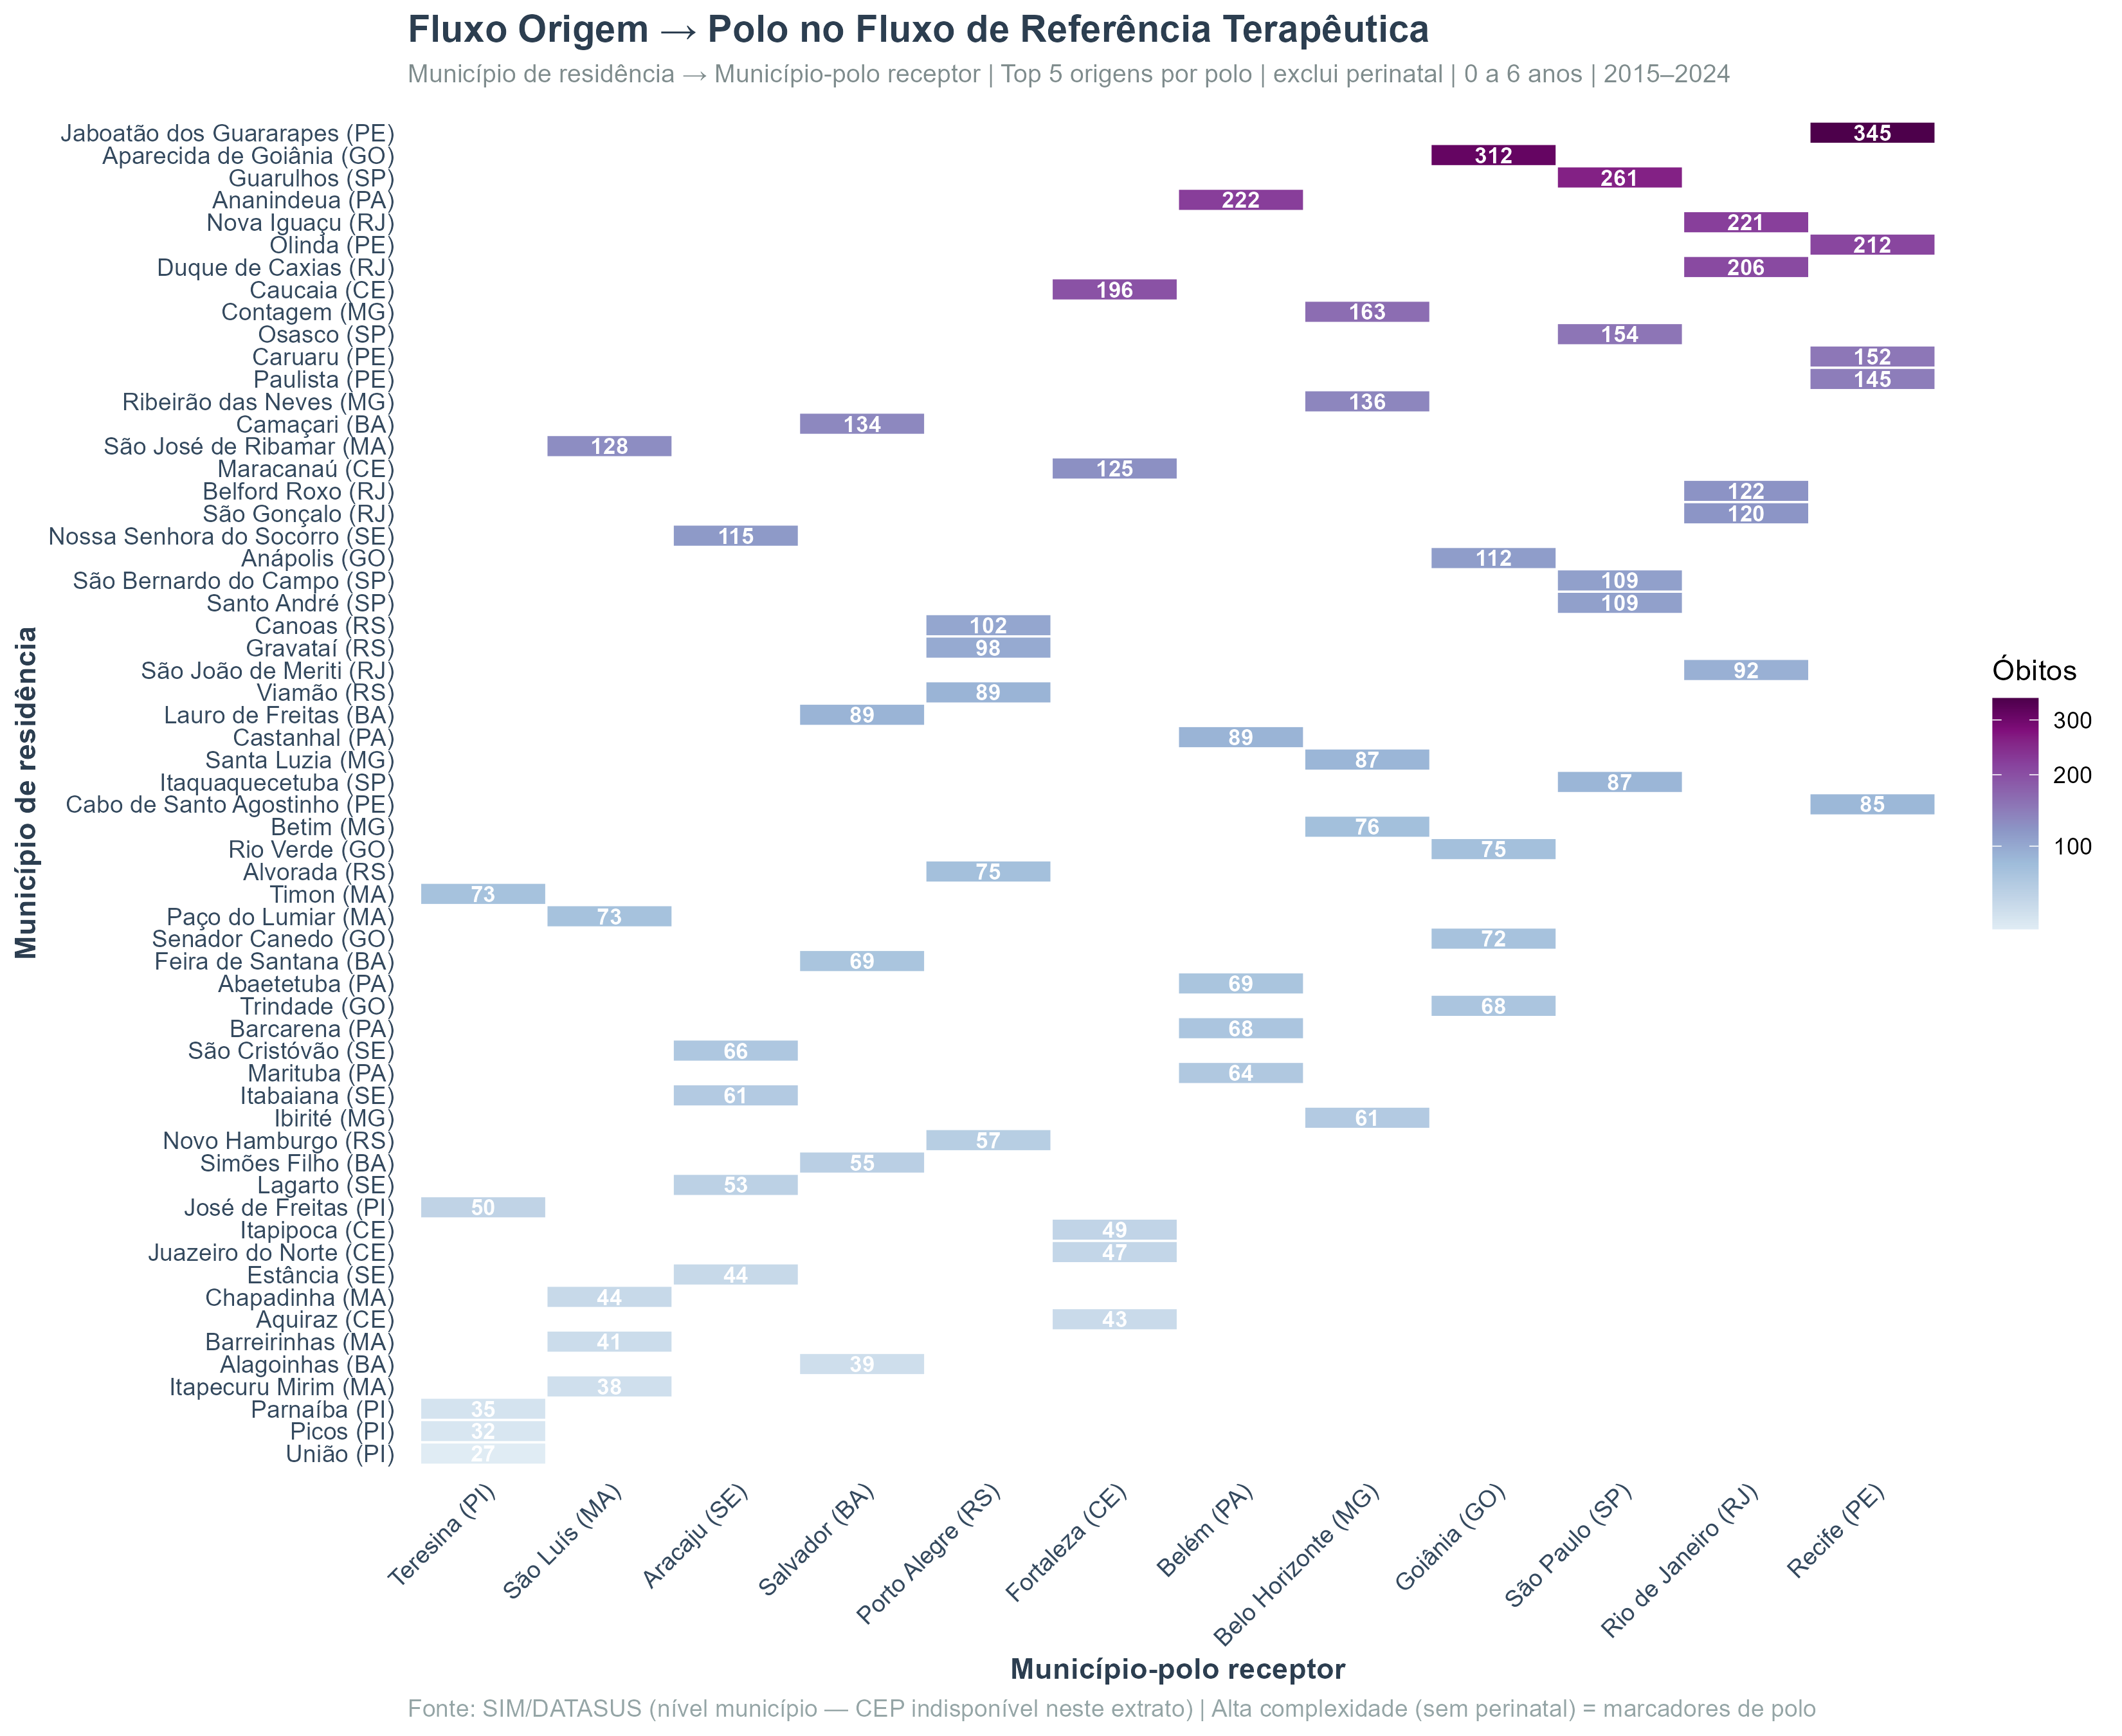
\includegraphics[width=0.7\linewidth,height=\textheight,keepaspectratio]{../outputs/SIM/Fig12_Fluxo_CEP_Origem_Destino_Polos.png}

}

\caption{Fluxo Origem ao Polo por Município para Alta Complexidade,
2015-2024}

\end{figure}%
\end{frame}

\begin{frame}{Evolução de Internações na Primeira Infância}
\protect\phantomsection\label{evoluuxe7uxe3o-de-internauxe7uxf5es-na-primeira-infuxe2ncia}
\begin{itemize}
\tightlist
\item
  Fazer gráfico de taxa de internação e internação por milhares para
  menos que um ano, 1 a menos que 5 anos e 5 e 6 anos, como na visão
  geral; referência:
  https://data.unicef.org/resources/levels-and-trends-in-child-mortality-2024/
\end{itemize}
\end{frame}

\begin{frame}{Evolução de Internações para Neonatal}
\protect\phantomsection\label{evoluuxe7uxe3o-de-internauxe7uxf5es-para-neonatal}
\begin{itemize}
\tightlist
\item
  Fazer gráfico de taxa de internação e internação por milhares para
  neotanal por neonatal precoce, neonatal tardia, pós-neonatal
\end{itemize}
\end{frame}

\begin{frame}{Evolução da Internações para Crianças}
\protect\phantomsection\label{evoluuxe7uxe3o-da-internauxe7uxf5es-para-crianuxe7as}
\begin{itemize}
\tightlist
\item
  Fazer gráfico de taxa de internação e internação por milhares para
  crianças: 1 a \textless{} 2 anos, 2 a \textless{} 5 anos e 5 e 6 anos
\end{itemize}
\end{frame}

\begin{frame}{Evolução das Causas de Internação}
\protect\phantomsection\label{evoluuxe7uxe3o-das-causas-de-internauxe7uxe3o}
\begin{figure}[H]

{\centering 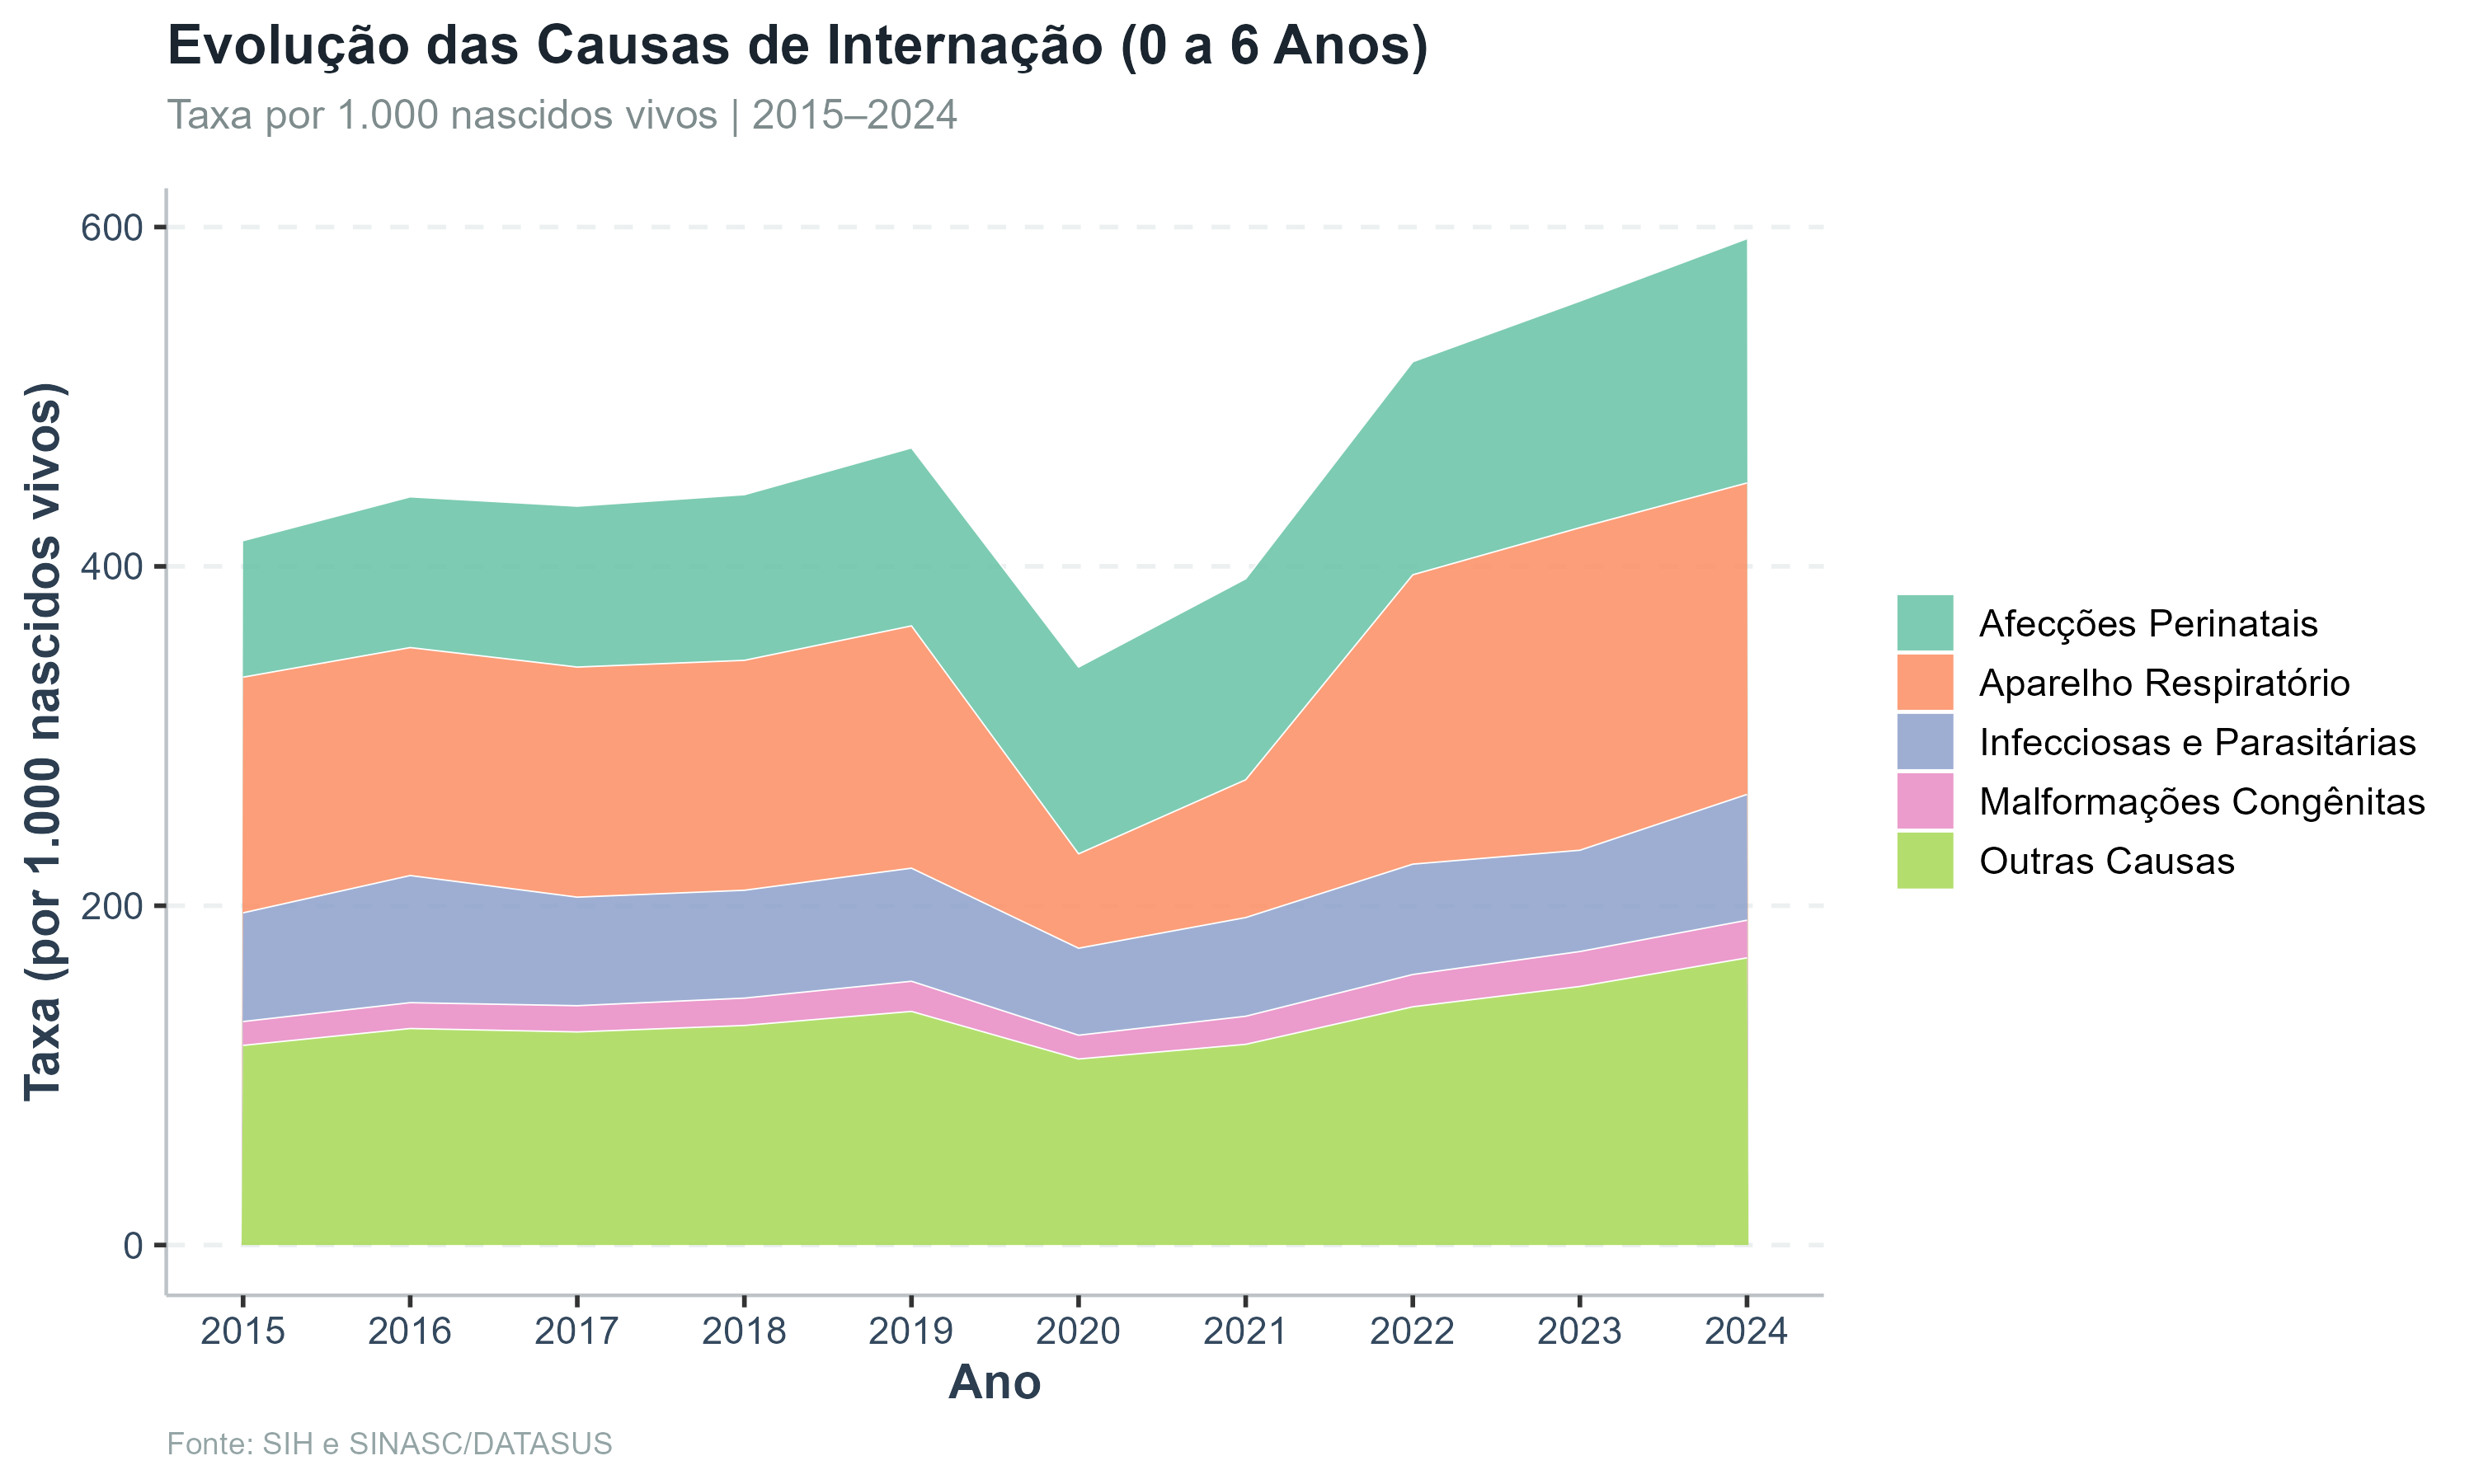
\includegraphics[width=0.9\linewidth,height=\textheight,keepaspectratio]{../outputs/SIH/Fig02_Evolucao_Causas_Taxa.png}

}

\caption{Evolução das Causas de Internação: Taxa por 1.000 Nascidos
Vivos, 2015-2024}

\end{figure}%
\end{frame}

\begin{frame}{Causas Prioritárias de Internação por Faixa Etária}
\protect\phantomsection\label{causas-priorituxe1rias-de-internauxe7uxe3o-por-faixa-etuxe1ria}
\begin{figure}[H]

{\centering 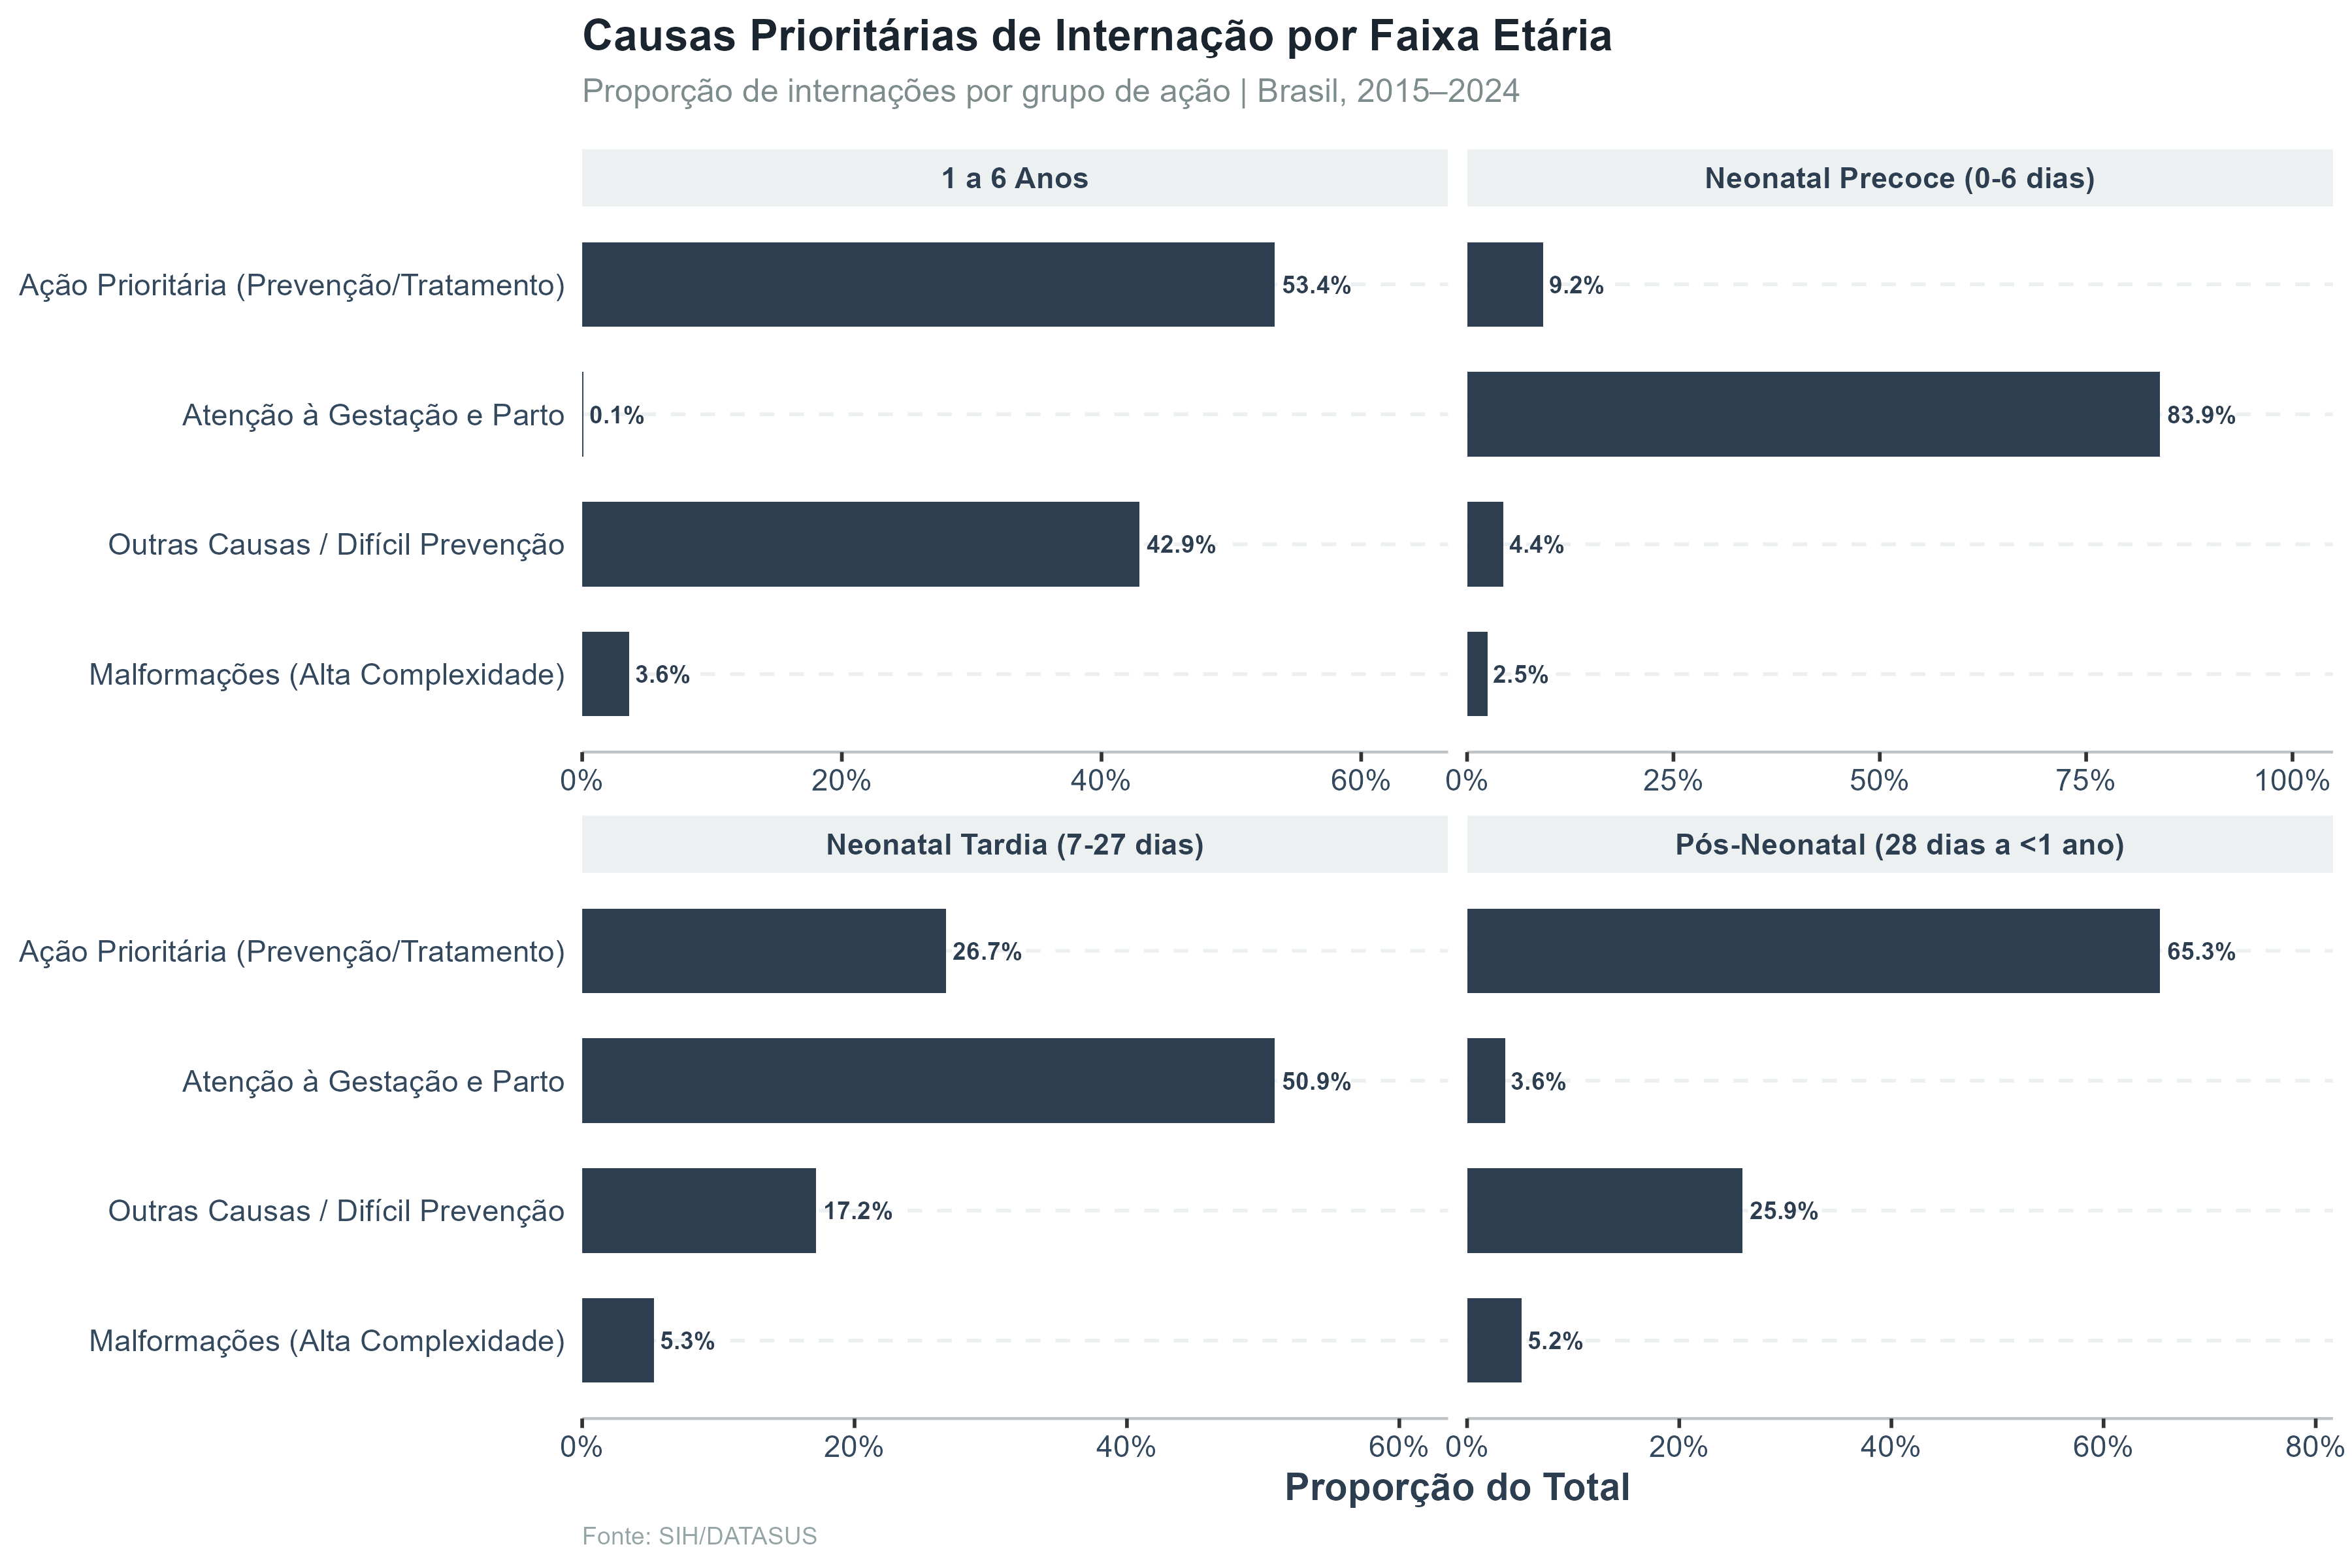
\includegraphics[width=0.9\linewidth,height=\textheight,keepaspectratio]{../outputs/SIH/Fig03_Causas_Prioritarias_por_Faixa.png}

}

\caption{Causas Prioritárias de Internação por Faixa Etária, 2015-2024}

\end{figure}%
\end{frame}

\begin{frame}{Análise Espacial e Desigualdades Regionais nas
Internações}
\protect\phantomsection\label{anuxe1lise-espacial-e-desigualdades-regionais-nas-internauxe7uxf5es}
\begin{figure}[H]

{\centering 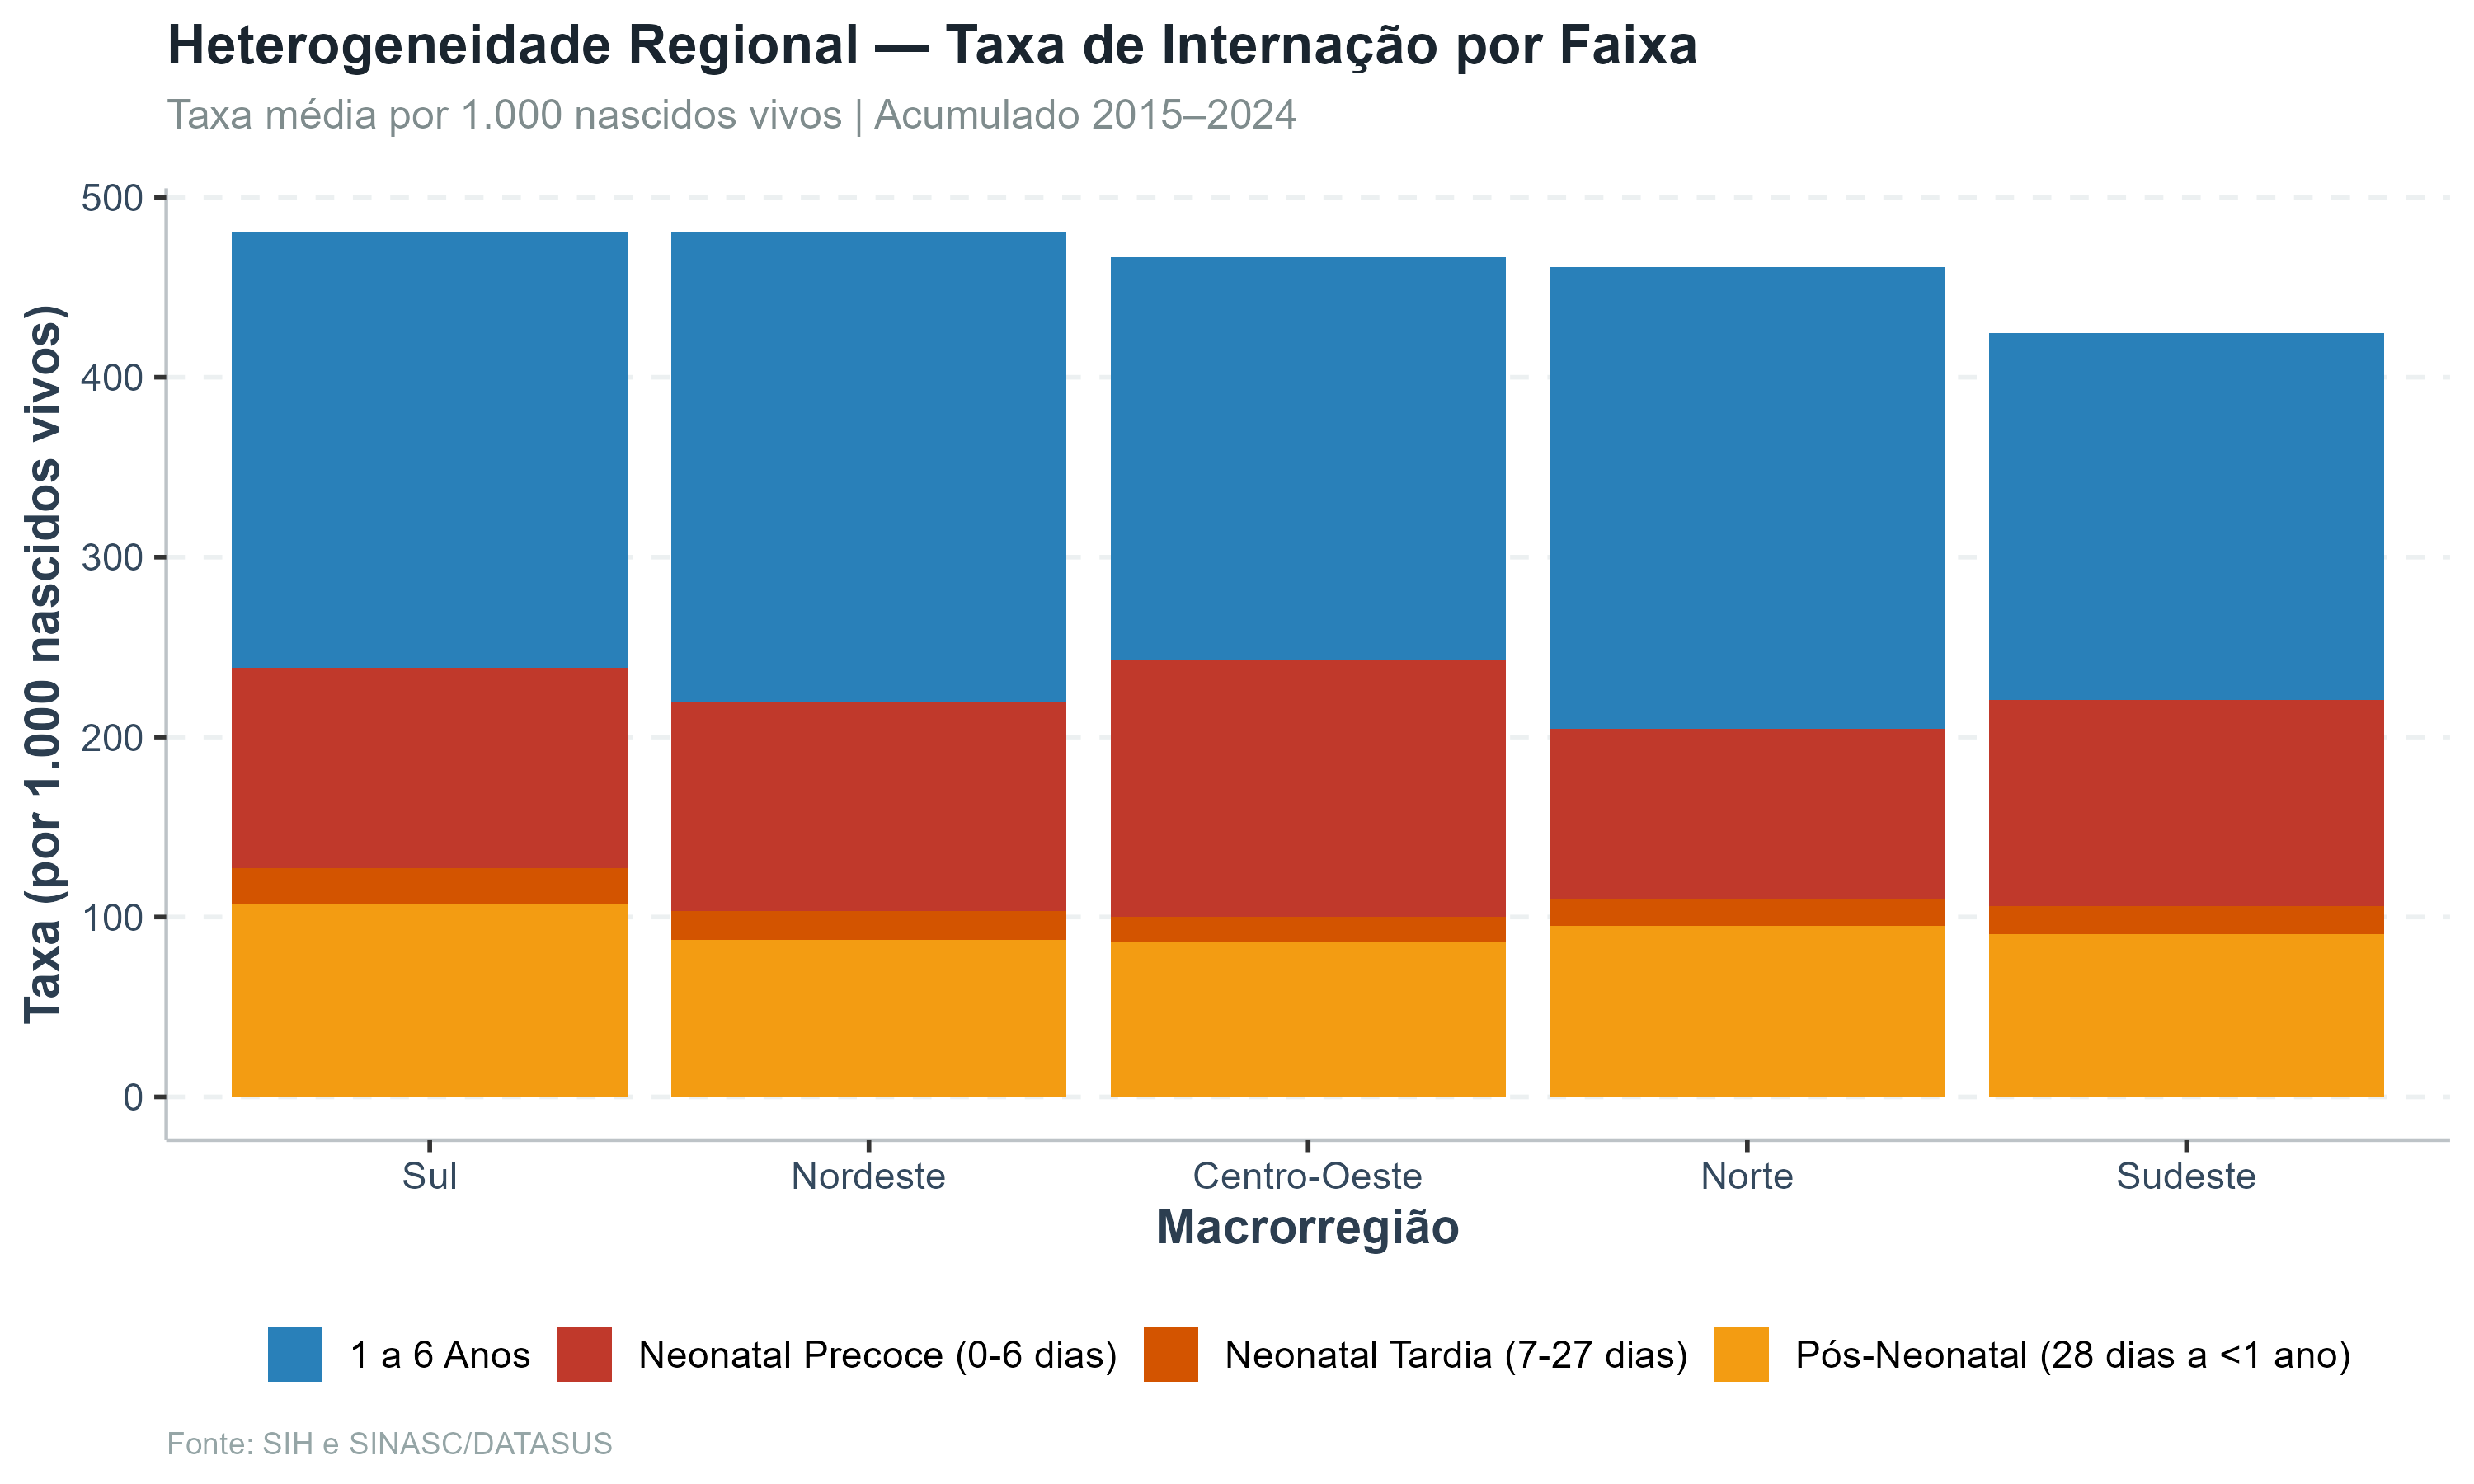
\includegraphics[width=0.9\linewidth,height=\textheight,keepaspectratio]{../outputs/SIH/Fig04_Heterogeneidade_Macro_Taxa.png}

}

\caption{Heterogeneidade Regional da Taxa de Internação, 2015-2024}

\end{figure}%
\end{frame}

\begin{frame}{Análise Espacial e Desigualdades Regionais nas
Internações}
\protect\phantomsection\label{anuxe1lise-espacial-e-desigualdades-regionais-nas-internauxe7uxf5es-1}
\begin{figure}[H]

{\centering 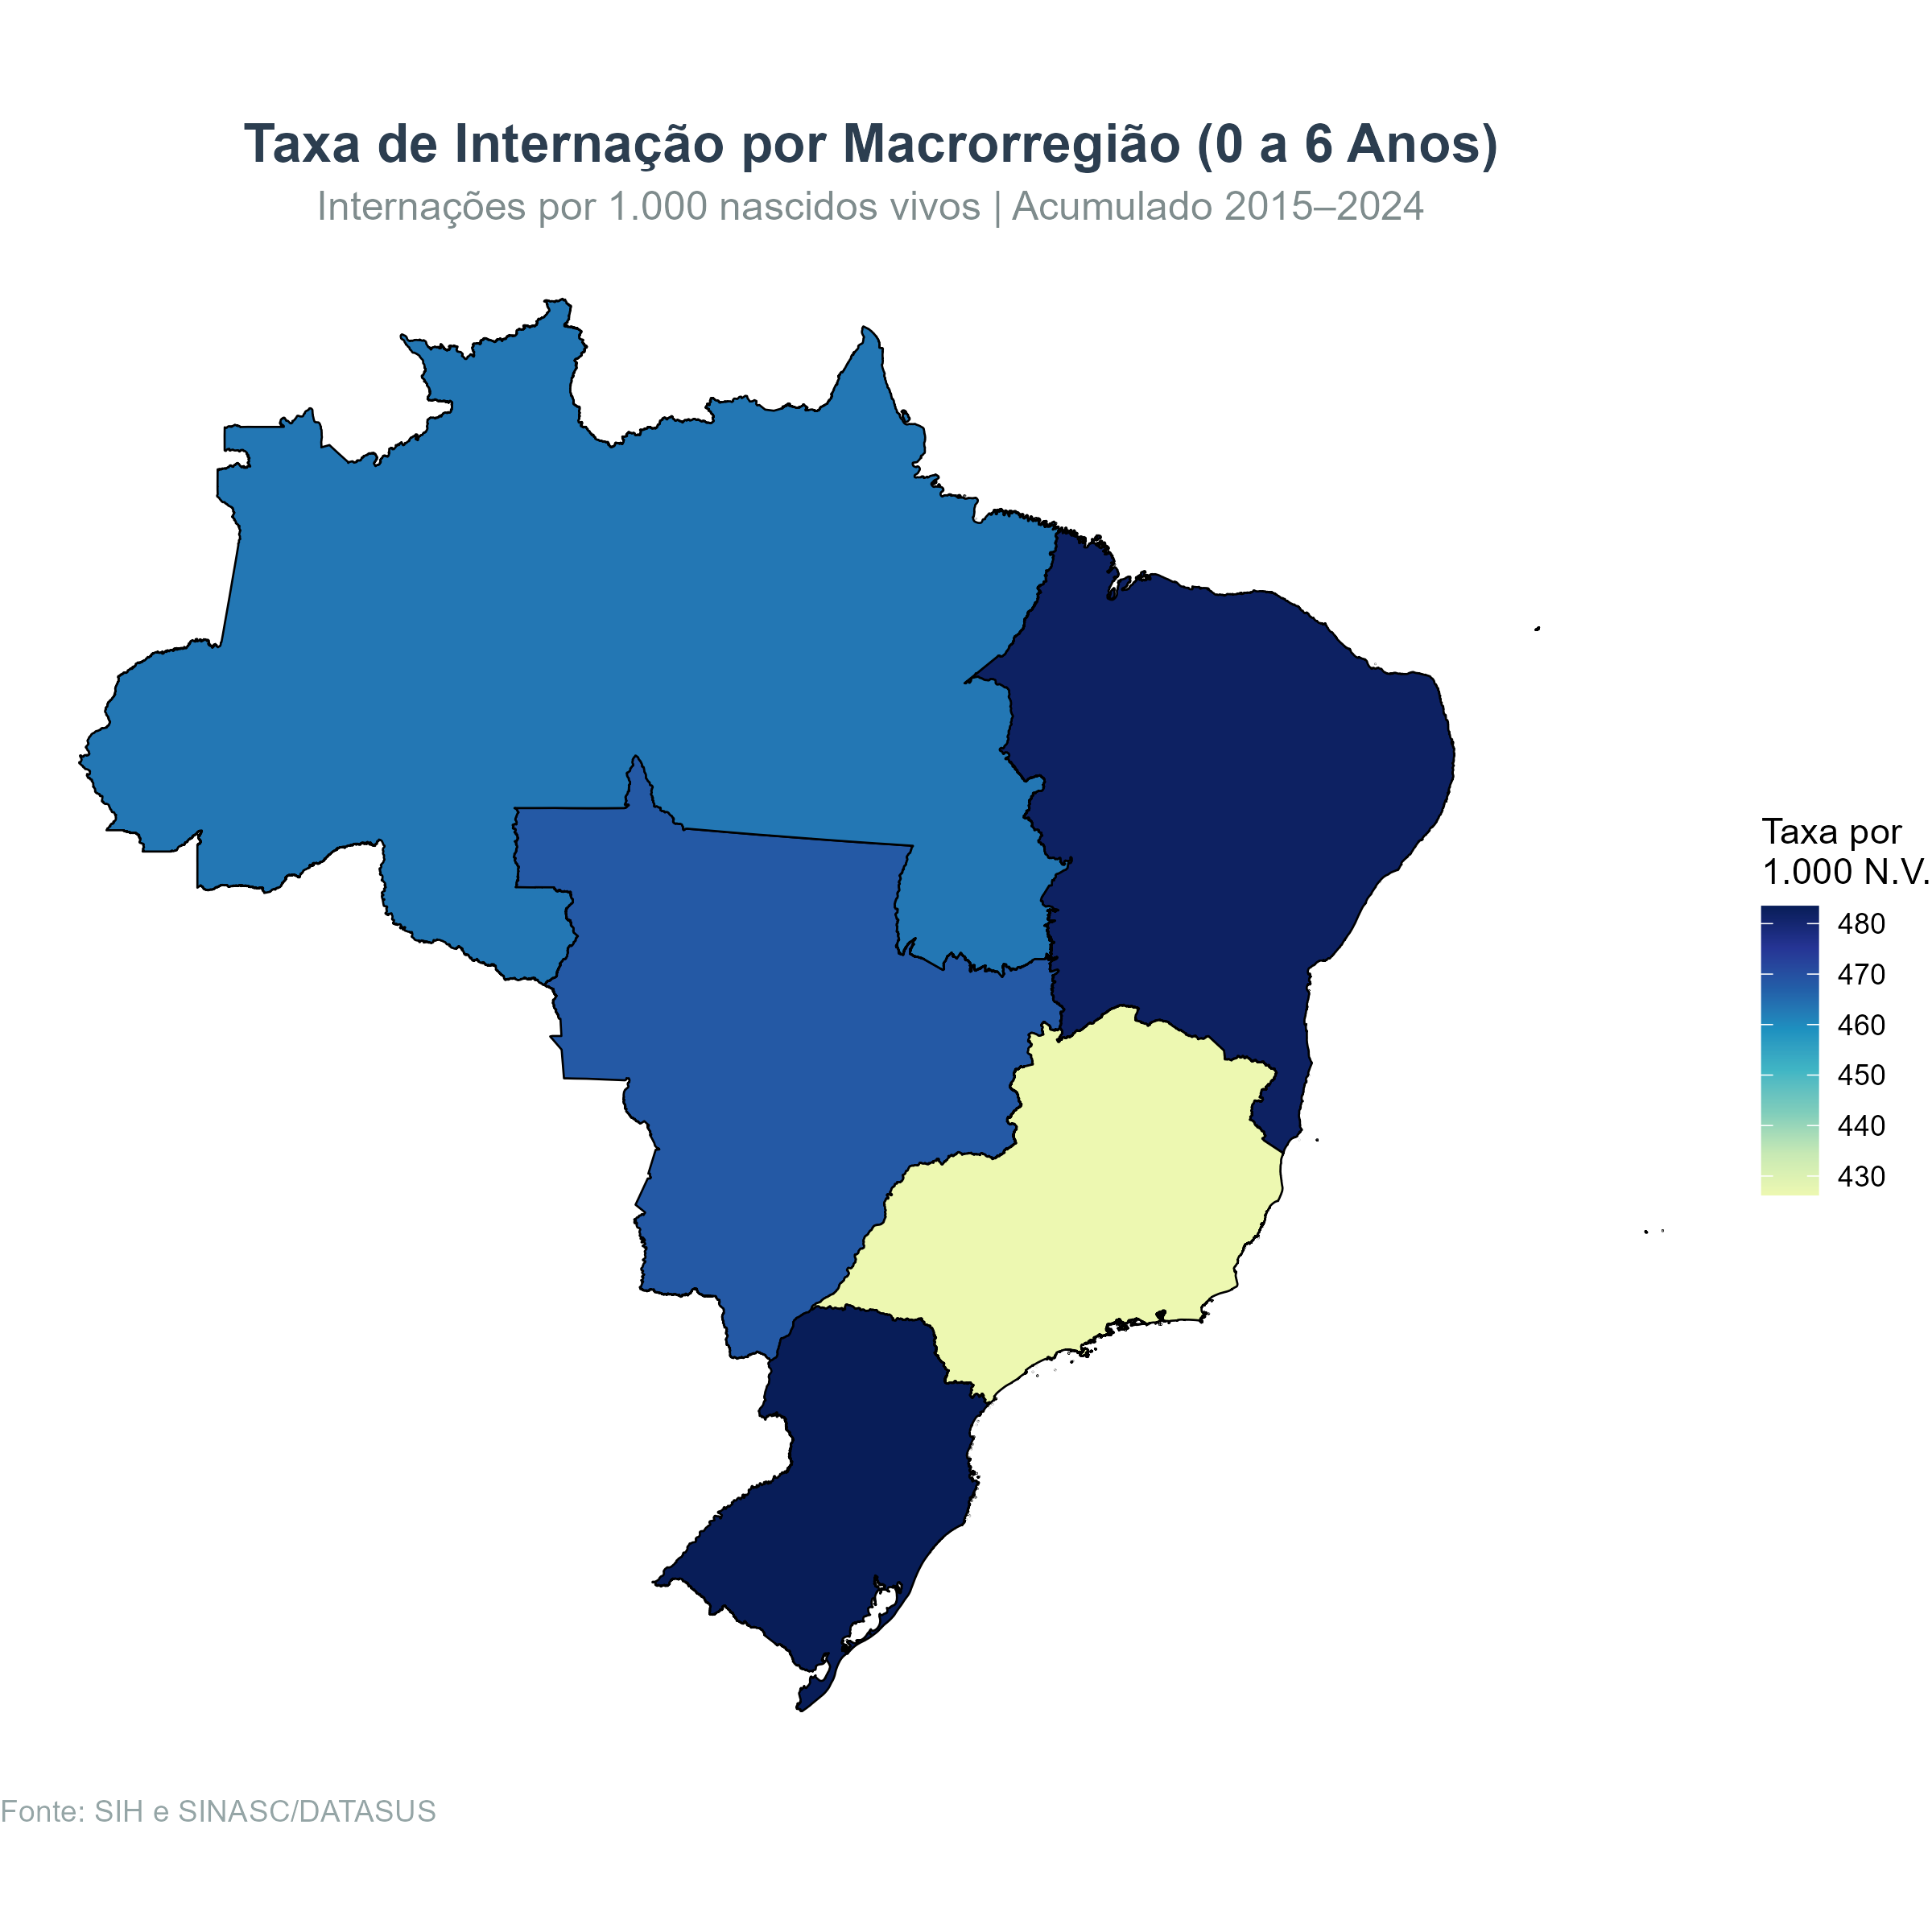
\includegraphics[width=0.6\linewidth,height=\textheight,keepaspectratio]{../outputs/SIH/Fig06_Mapa_Taxa_Macrorregiao.png}

}

\caption{Distribuição Espacial da Taxa de Internação por Macrorregião,
2015-2024}

\end{figure}%
\end{frame}

\begin{frame}{Análise Espacial e Desigualdades Regionais nas
Internações}
\protect\phantomsection\label{anuxe1lise-espacial-e-desigualdades-regionais-nas-internauxe7uxf5es-2}
\begin{figure}[H]

{\centering 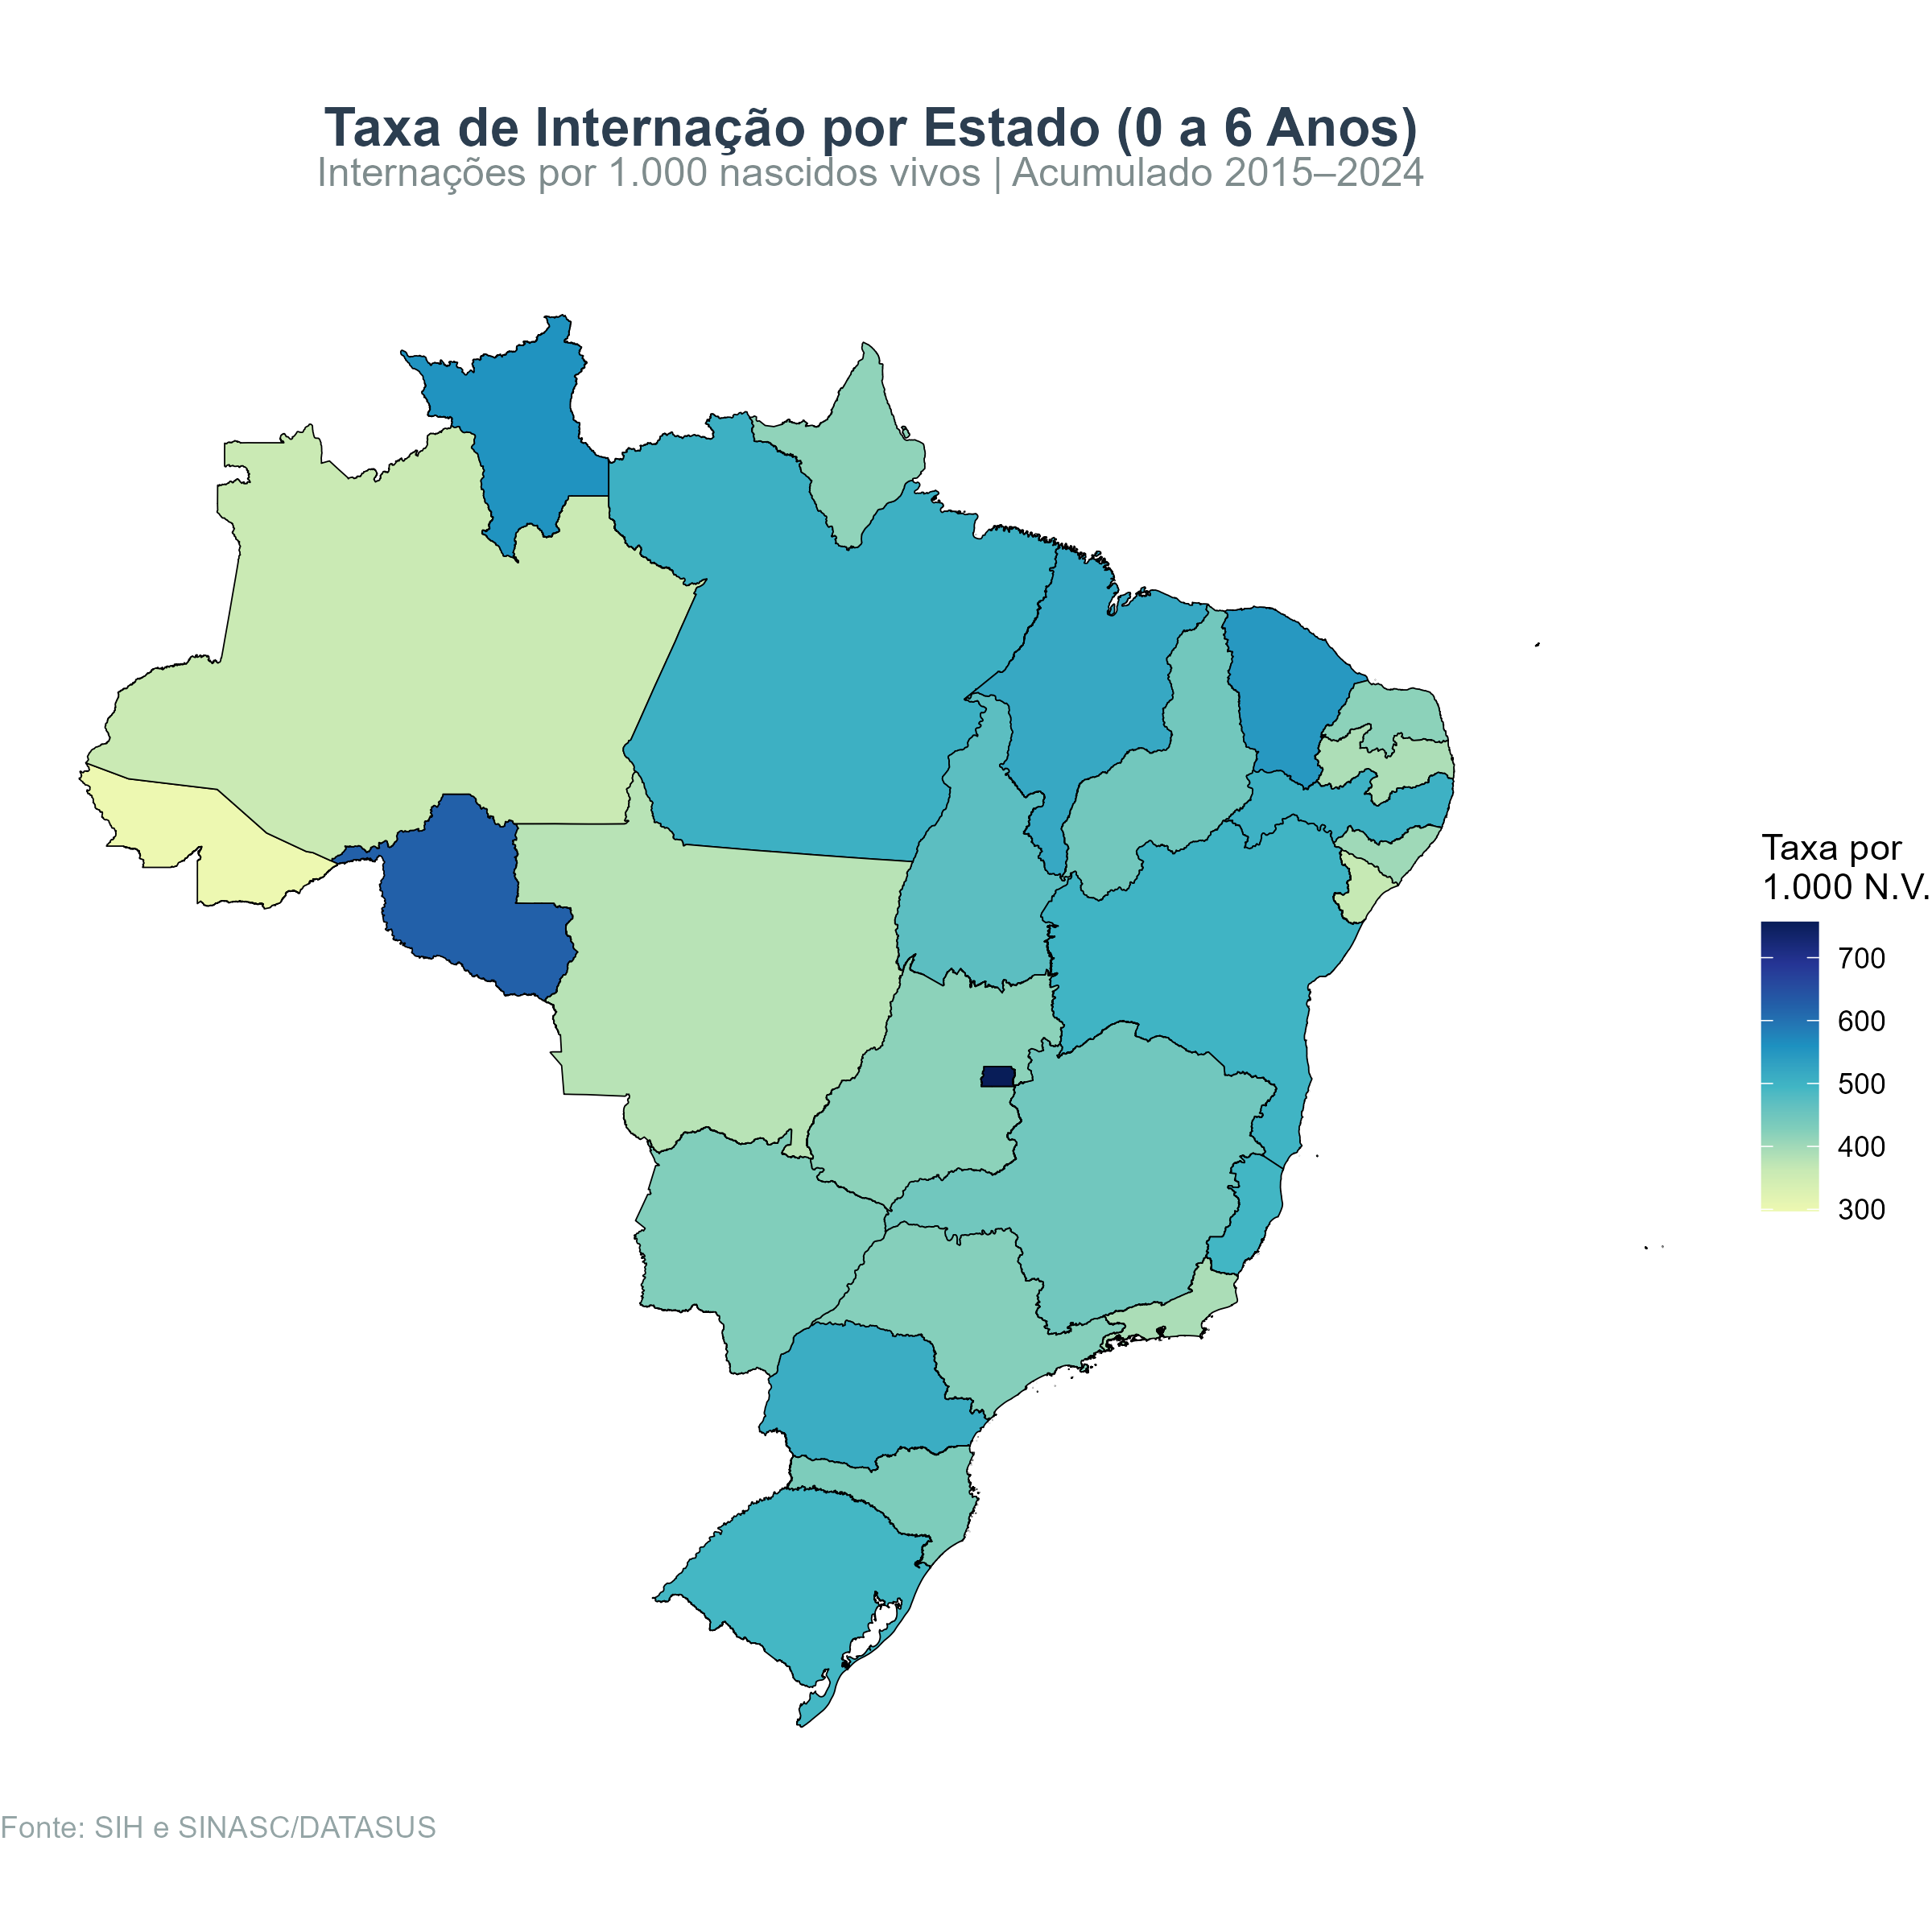
\includegraphics[width=0.6\linewidth,height=\textheight,keepaspectratio]{../outputs/SIH/Fig05_Mapa_Taxa_Estado.png}

}

\caption{Distribuição Espacial da Taxa de Internação por Estado,
2015-2024}

\end{figure}%
\end{frame}

\begin{frame}{Fluxos Assistenciais e Polos de Atendimento Infantil}
\protect\phantomsection\label{fluxos-assistenciais-e-polos-de-atendimento-infantil}
\begin{itemize}
\tightlist
\item
  A análise de fluxo das internações cruza o \textbf{município de
  residência} da criança com o \textbf{município de internação},
  permitindo identificar deslocamentos assistenciais, concentração de
  atendimentos em polos regionais e dependência de municípios receptores
  para o cuidado hospitalar infantil.
\end{itemize}
\end{frame}

\begin{frame}{Fluxos Assistenciais e Polos de Atendimento Infantil}
\protect\phantomsection\label{fluxos-assistenciais-e-polos-de-atendimento-infantil-1}
\begin{figure}[H]

{\centering 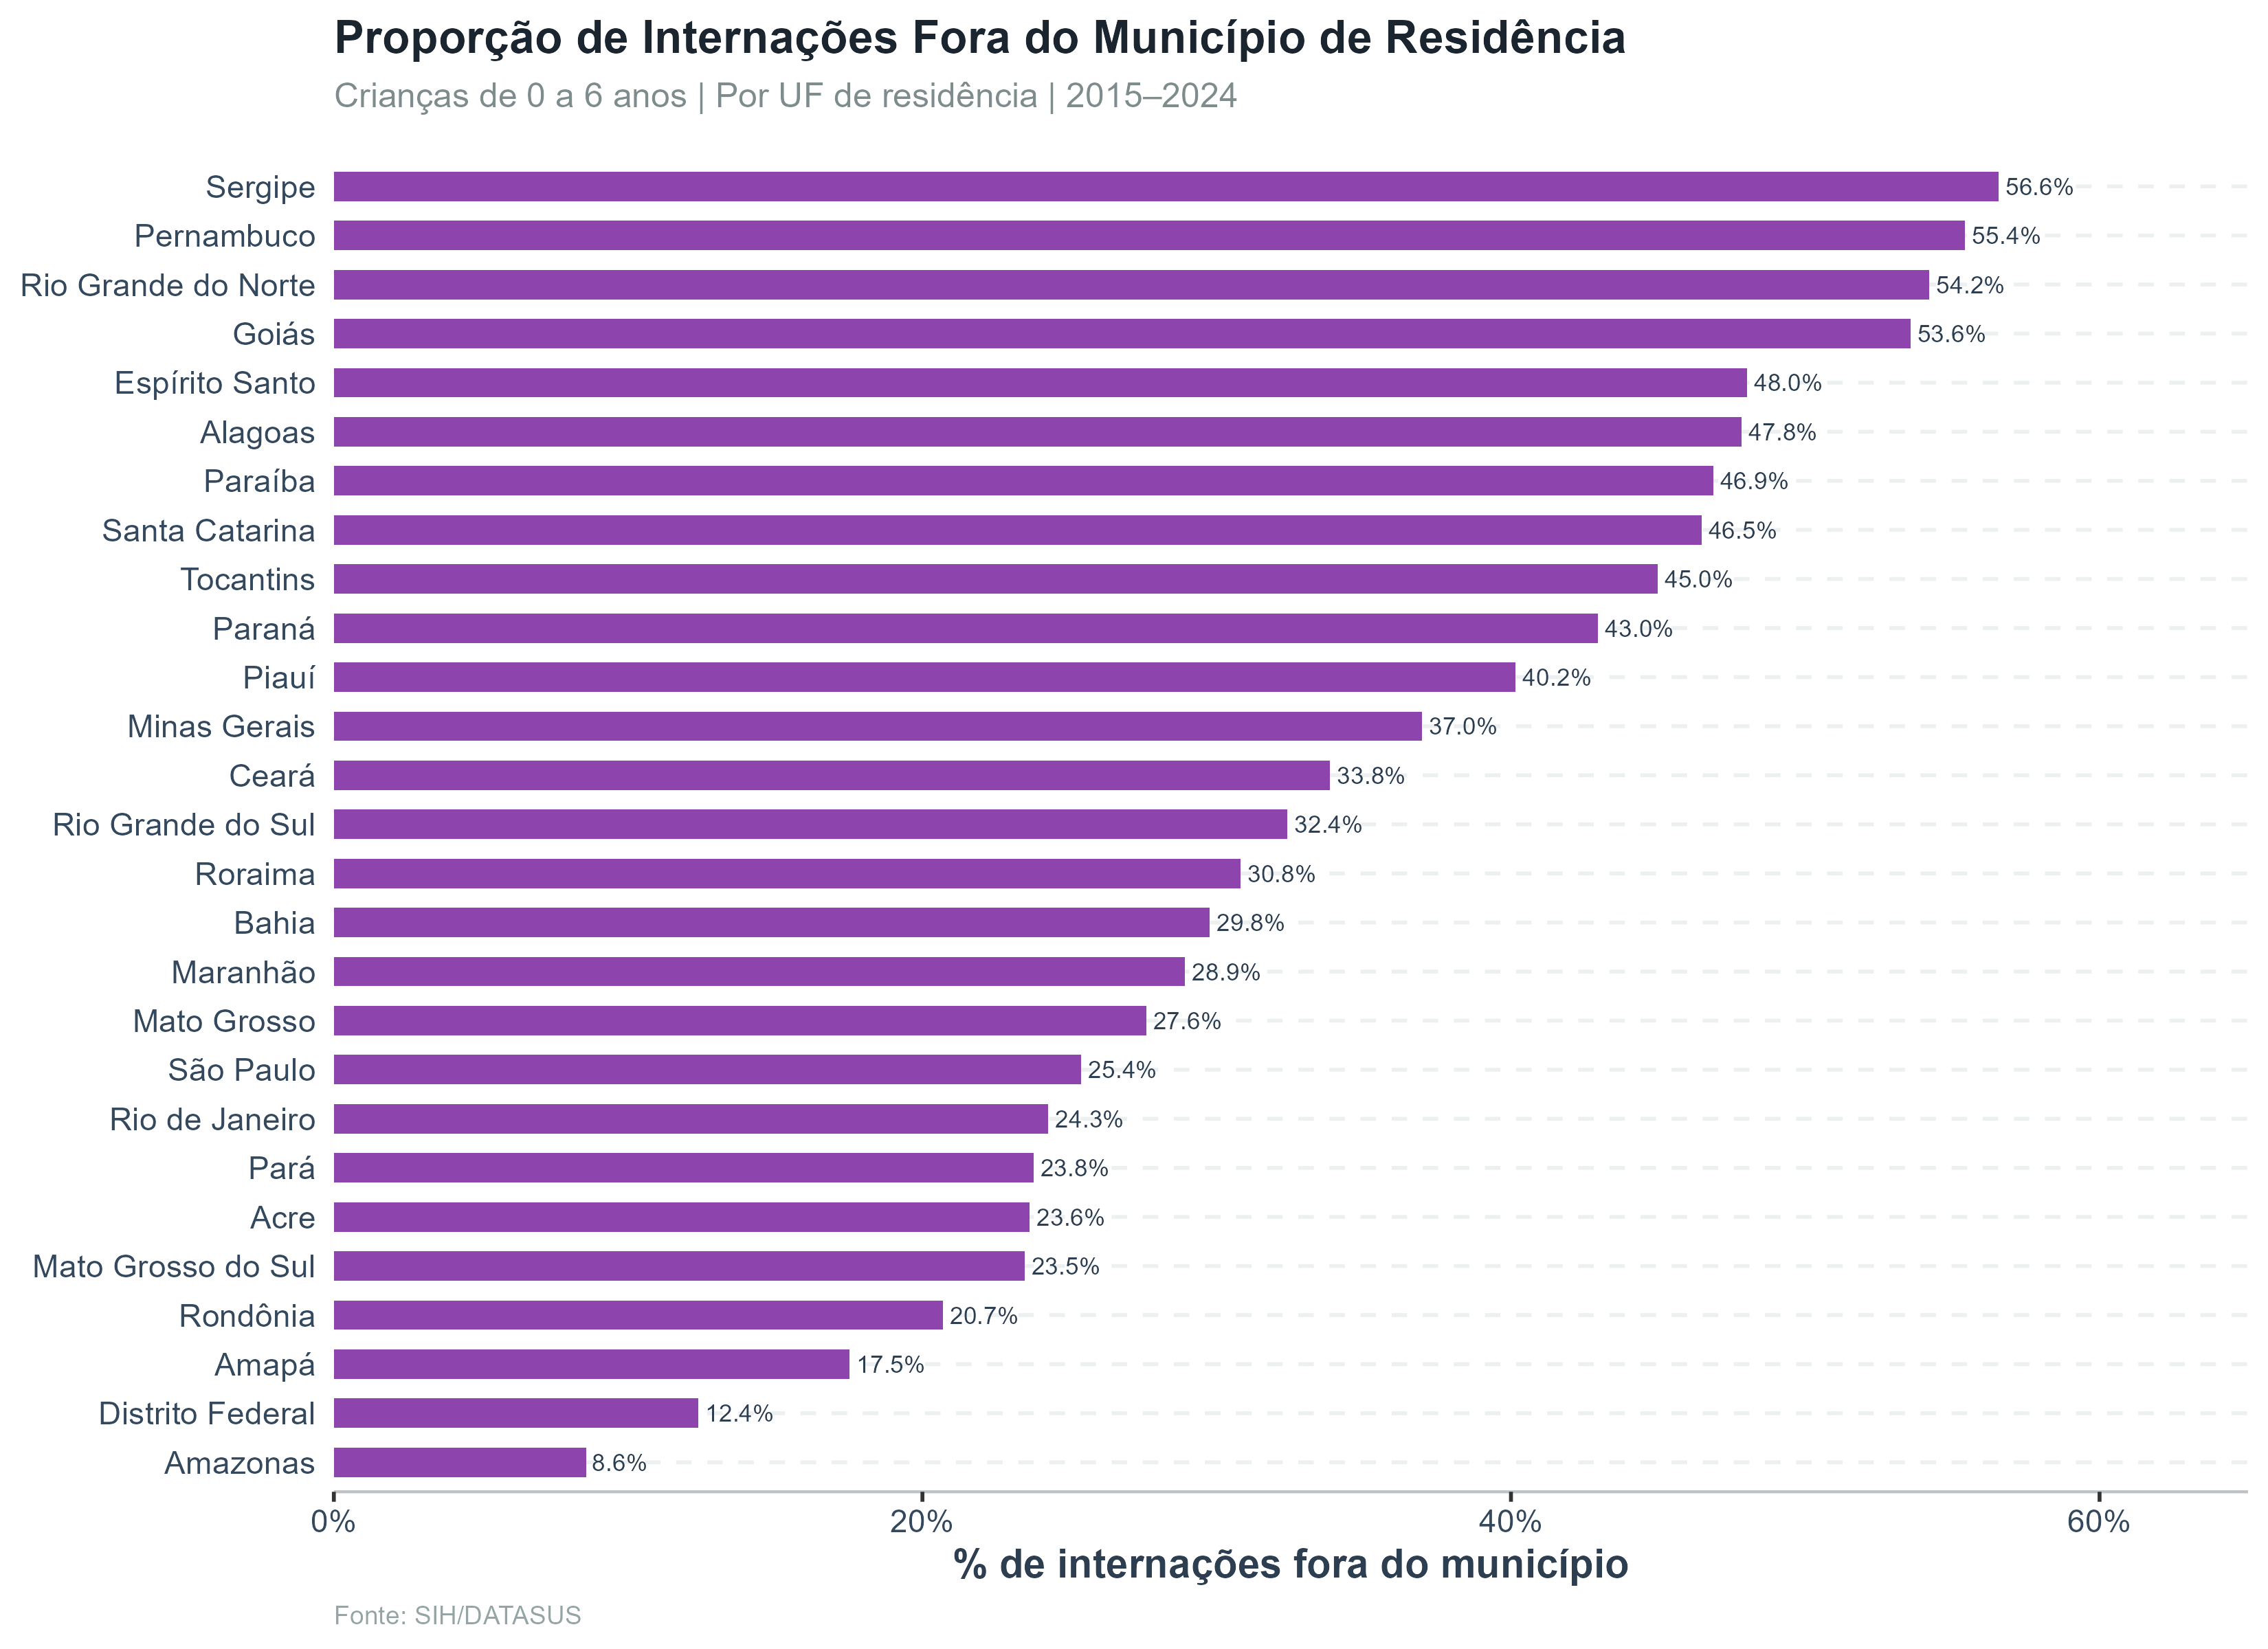
\includegraphics[width=0.6\linewidth,height=\textheight,keepaspectratio]{../outputs/SIH/Fig07_Fluxo_Internacoes_Fora_Municipio.png}

}

\caption{Proporção de Internações Fora do Município de Residência,
2015-2024}

\end{figure}%
\end{frame}

\begin{frame}{Fluxos Assistenciais e Polos de Atendimento Infantil}
\protect\phantomsection\label{fluxos-assistenciais-e-polos-de-atendimento-infantil-2}
\begin{figure}[H]

{\centering 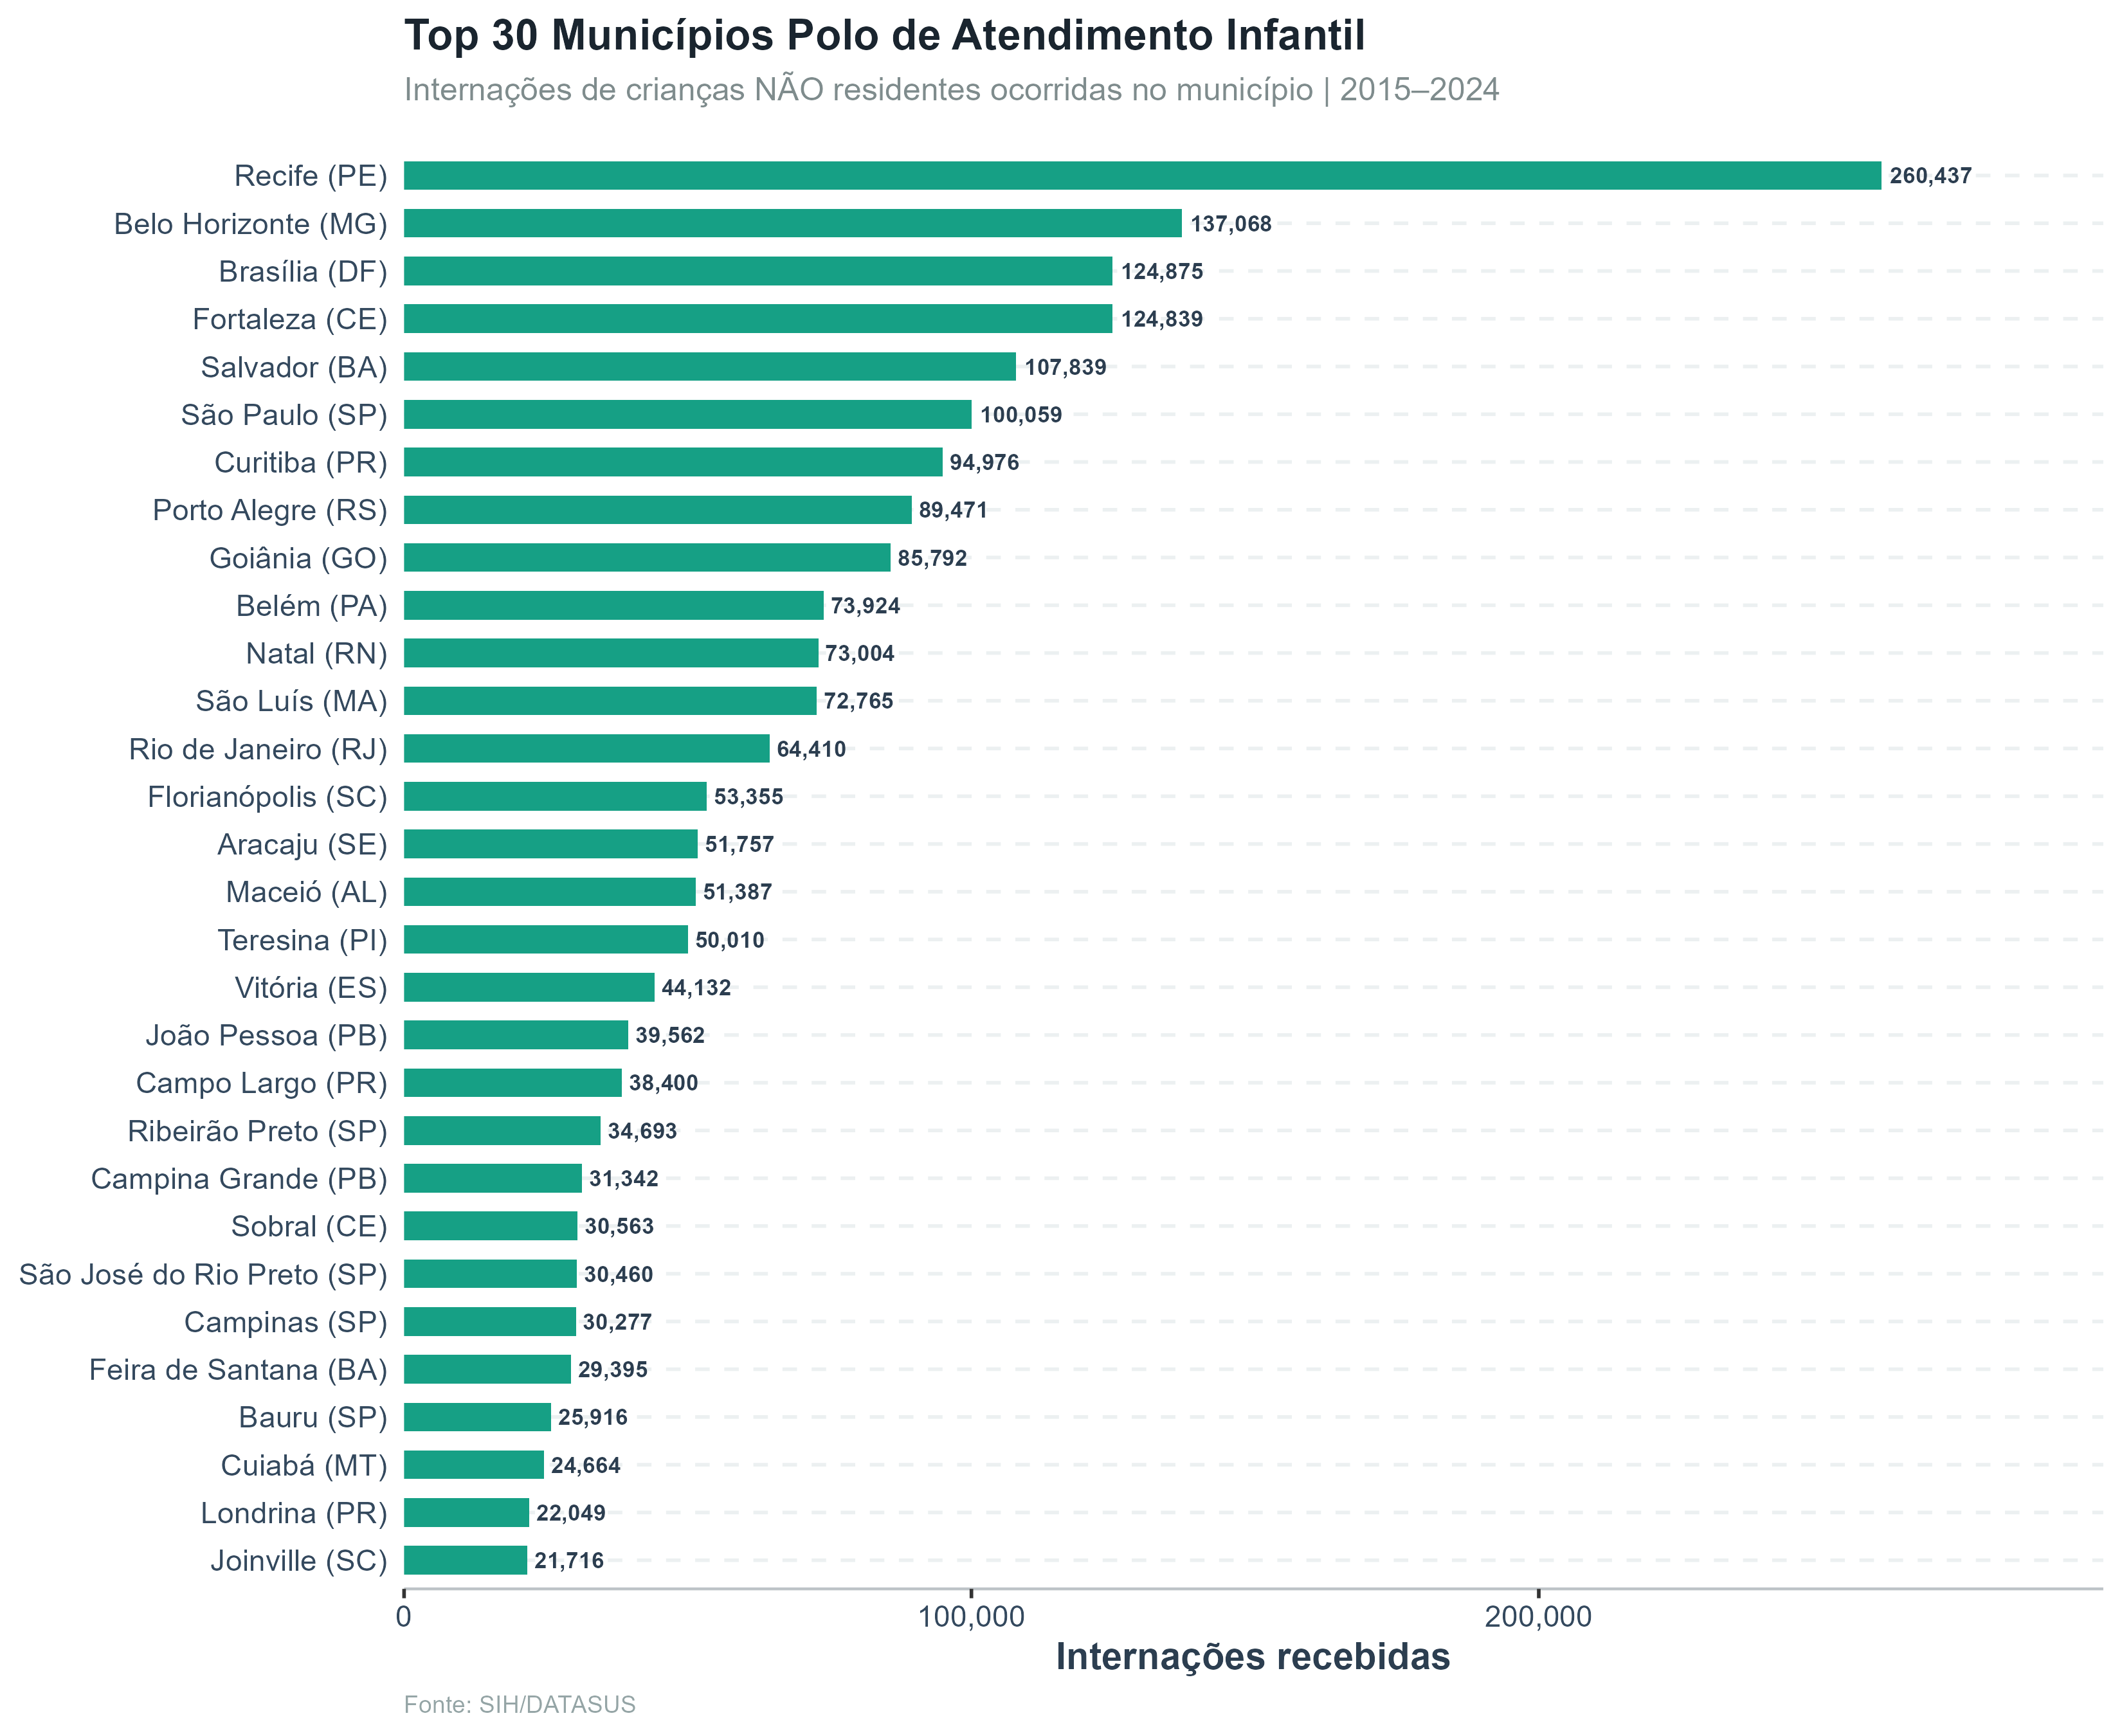
\includegraphics[width=0.6\linewidth,height=\textheight,keepaspectratio]{../outputs/SIH/Fig08_Polos_Saude_Infantil_Top30.png}

}

\caption{Municípios Polo de Saúde Infantil, 2015-2024}

\end{figure}%
\end{frame}

\begin{frame}{Fluxos Assistenciais e Polos de Atendimento Infantil}
\protect\phantomsection\label{fluxos-assistenciais-e-polos-de-atendimento-infantil-3}
\begin{figure}[H]

{\centering 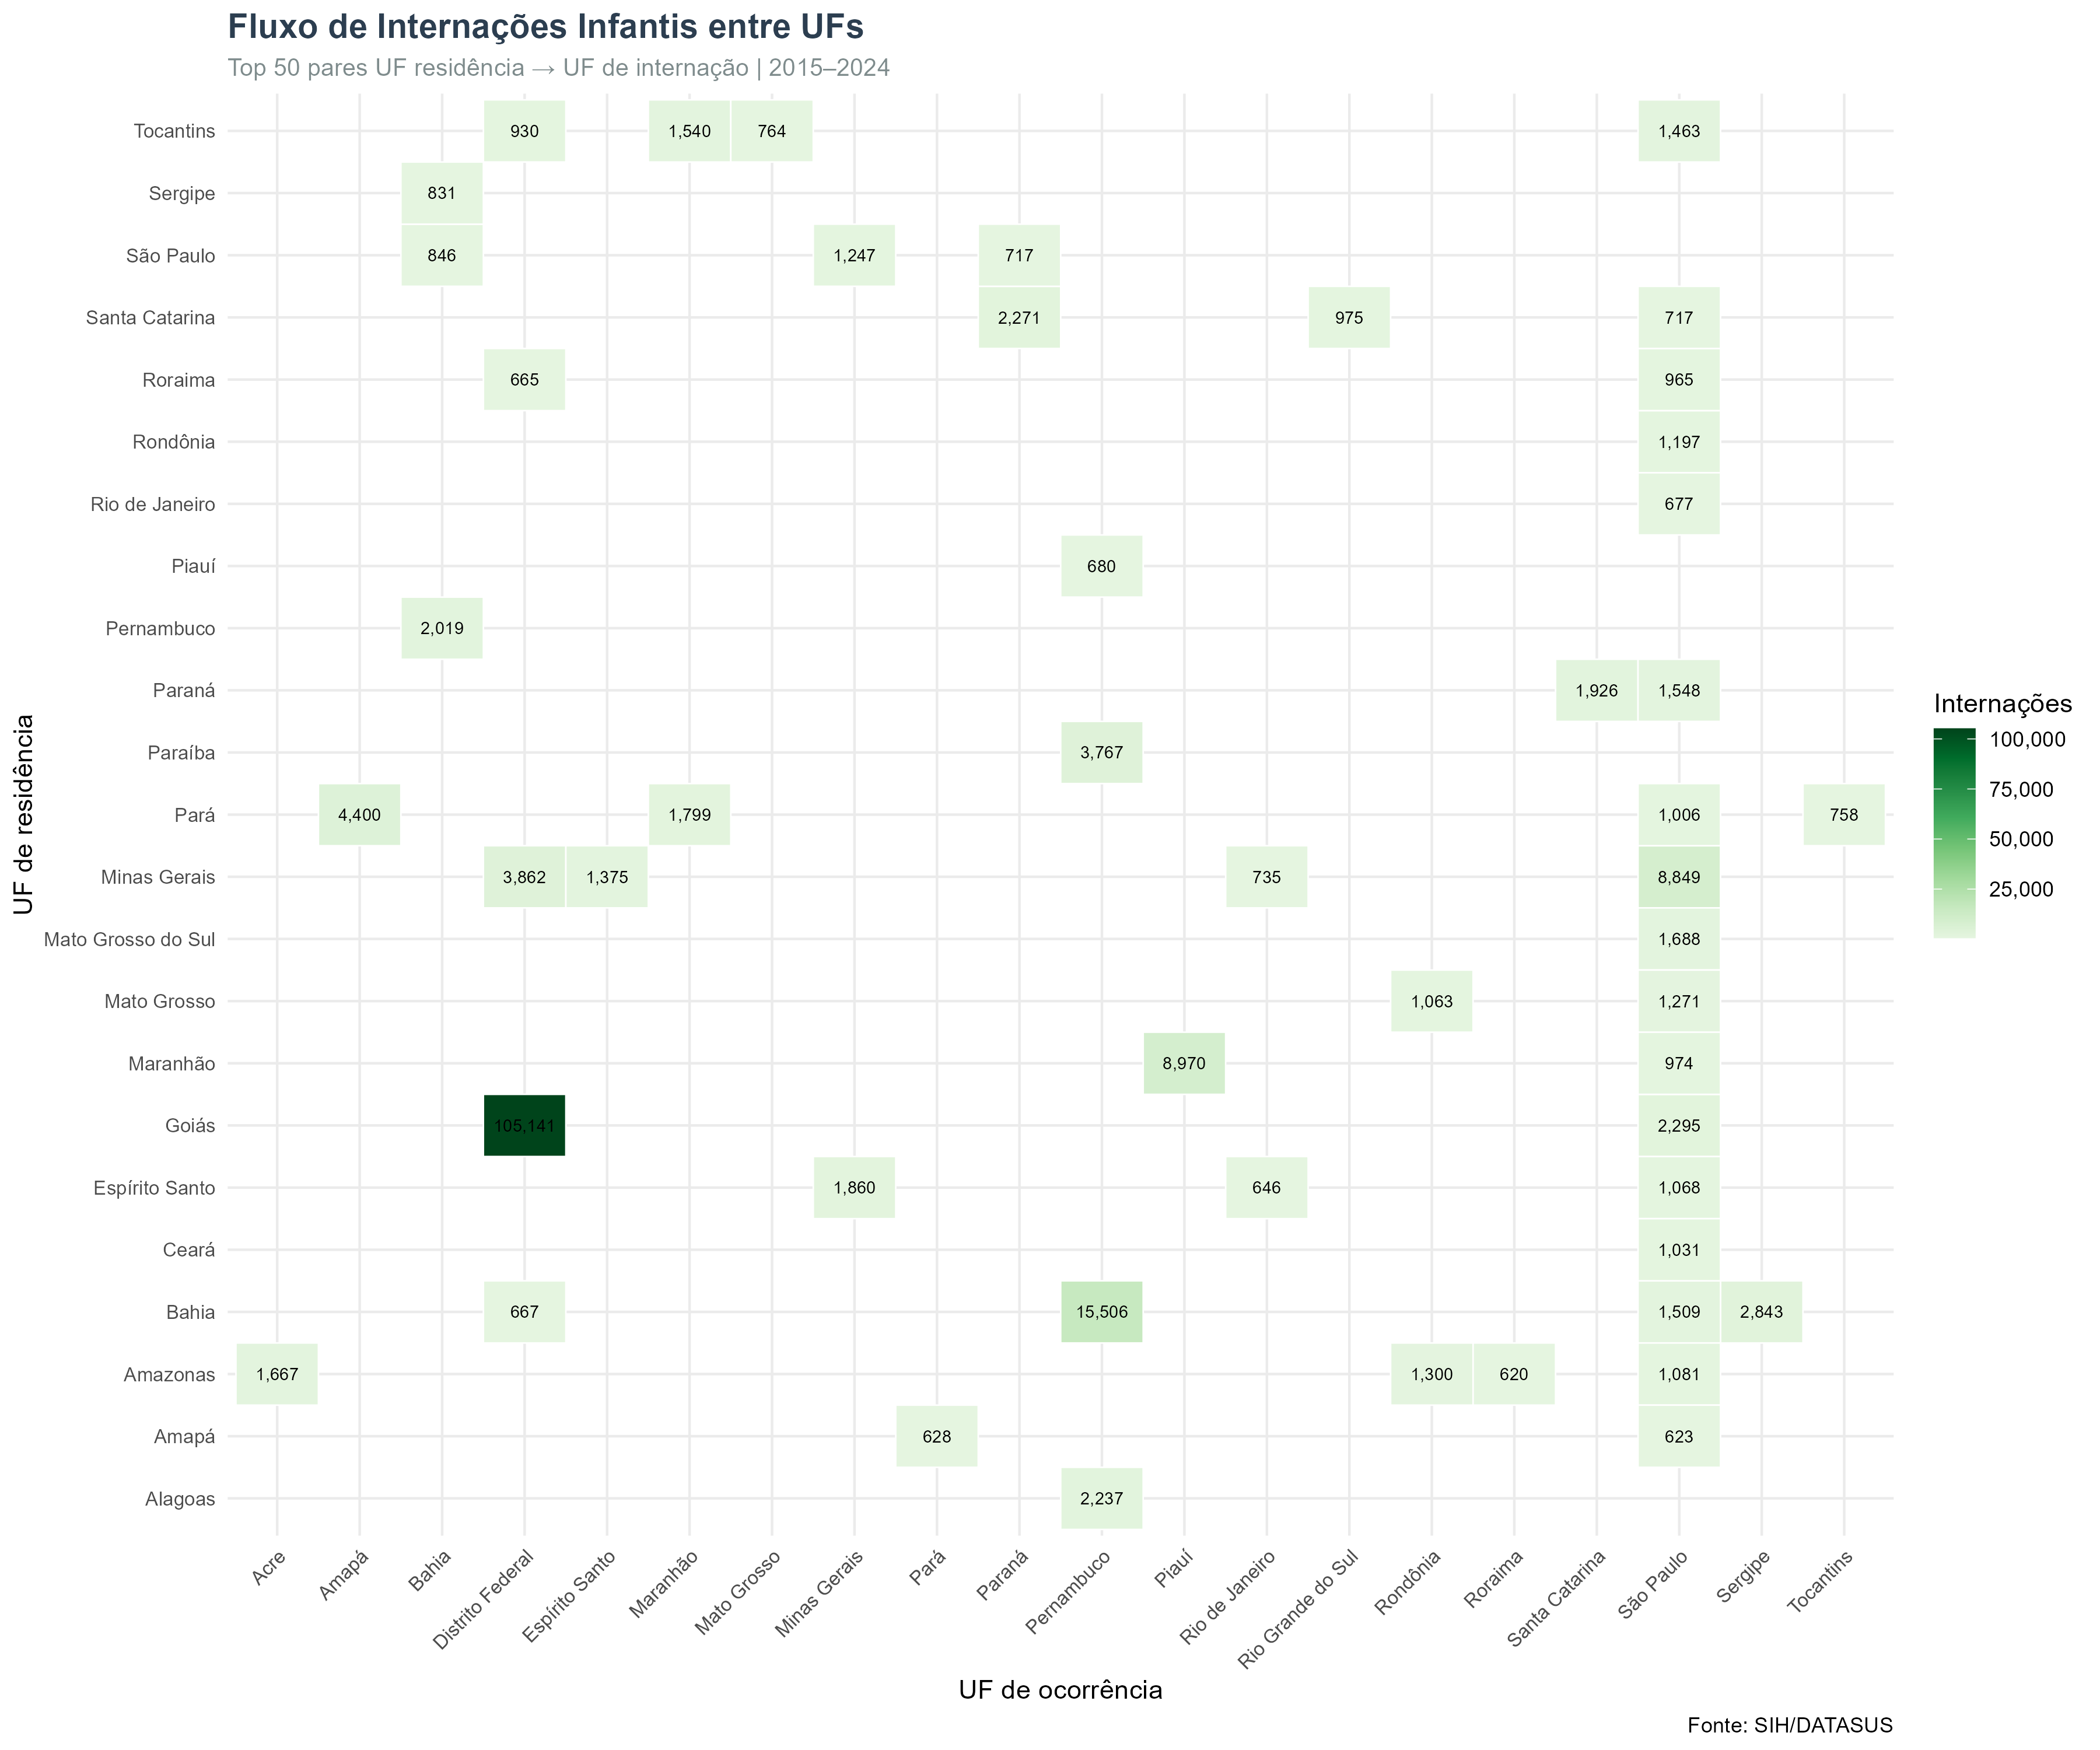
\includegraphics[width=0.7\linewidth,height=\textheight,keepaspectratio]{../outputs/SIH/Fig09_Heatmap_Fluxo_InterUF.png}

}

\caption{Fluxo de Mortalidade Infantil entre Estados, 2015-2024}

\end{figure}%
\end{frame}

\begin{frame}{Fluxos Assistenciais e Polos de Atendimento Infantil}
\protect\phantomsection\label{fluxos-assistenciais-e-polos-de-atendimento-infantil-4}
\begin{figure}[H]

{\centering 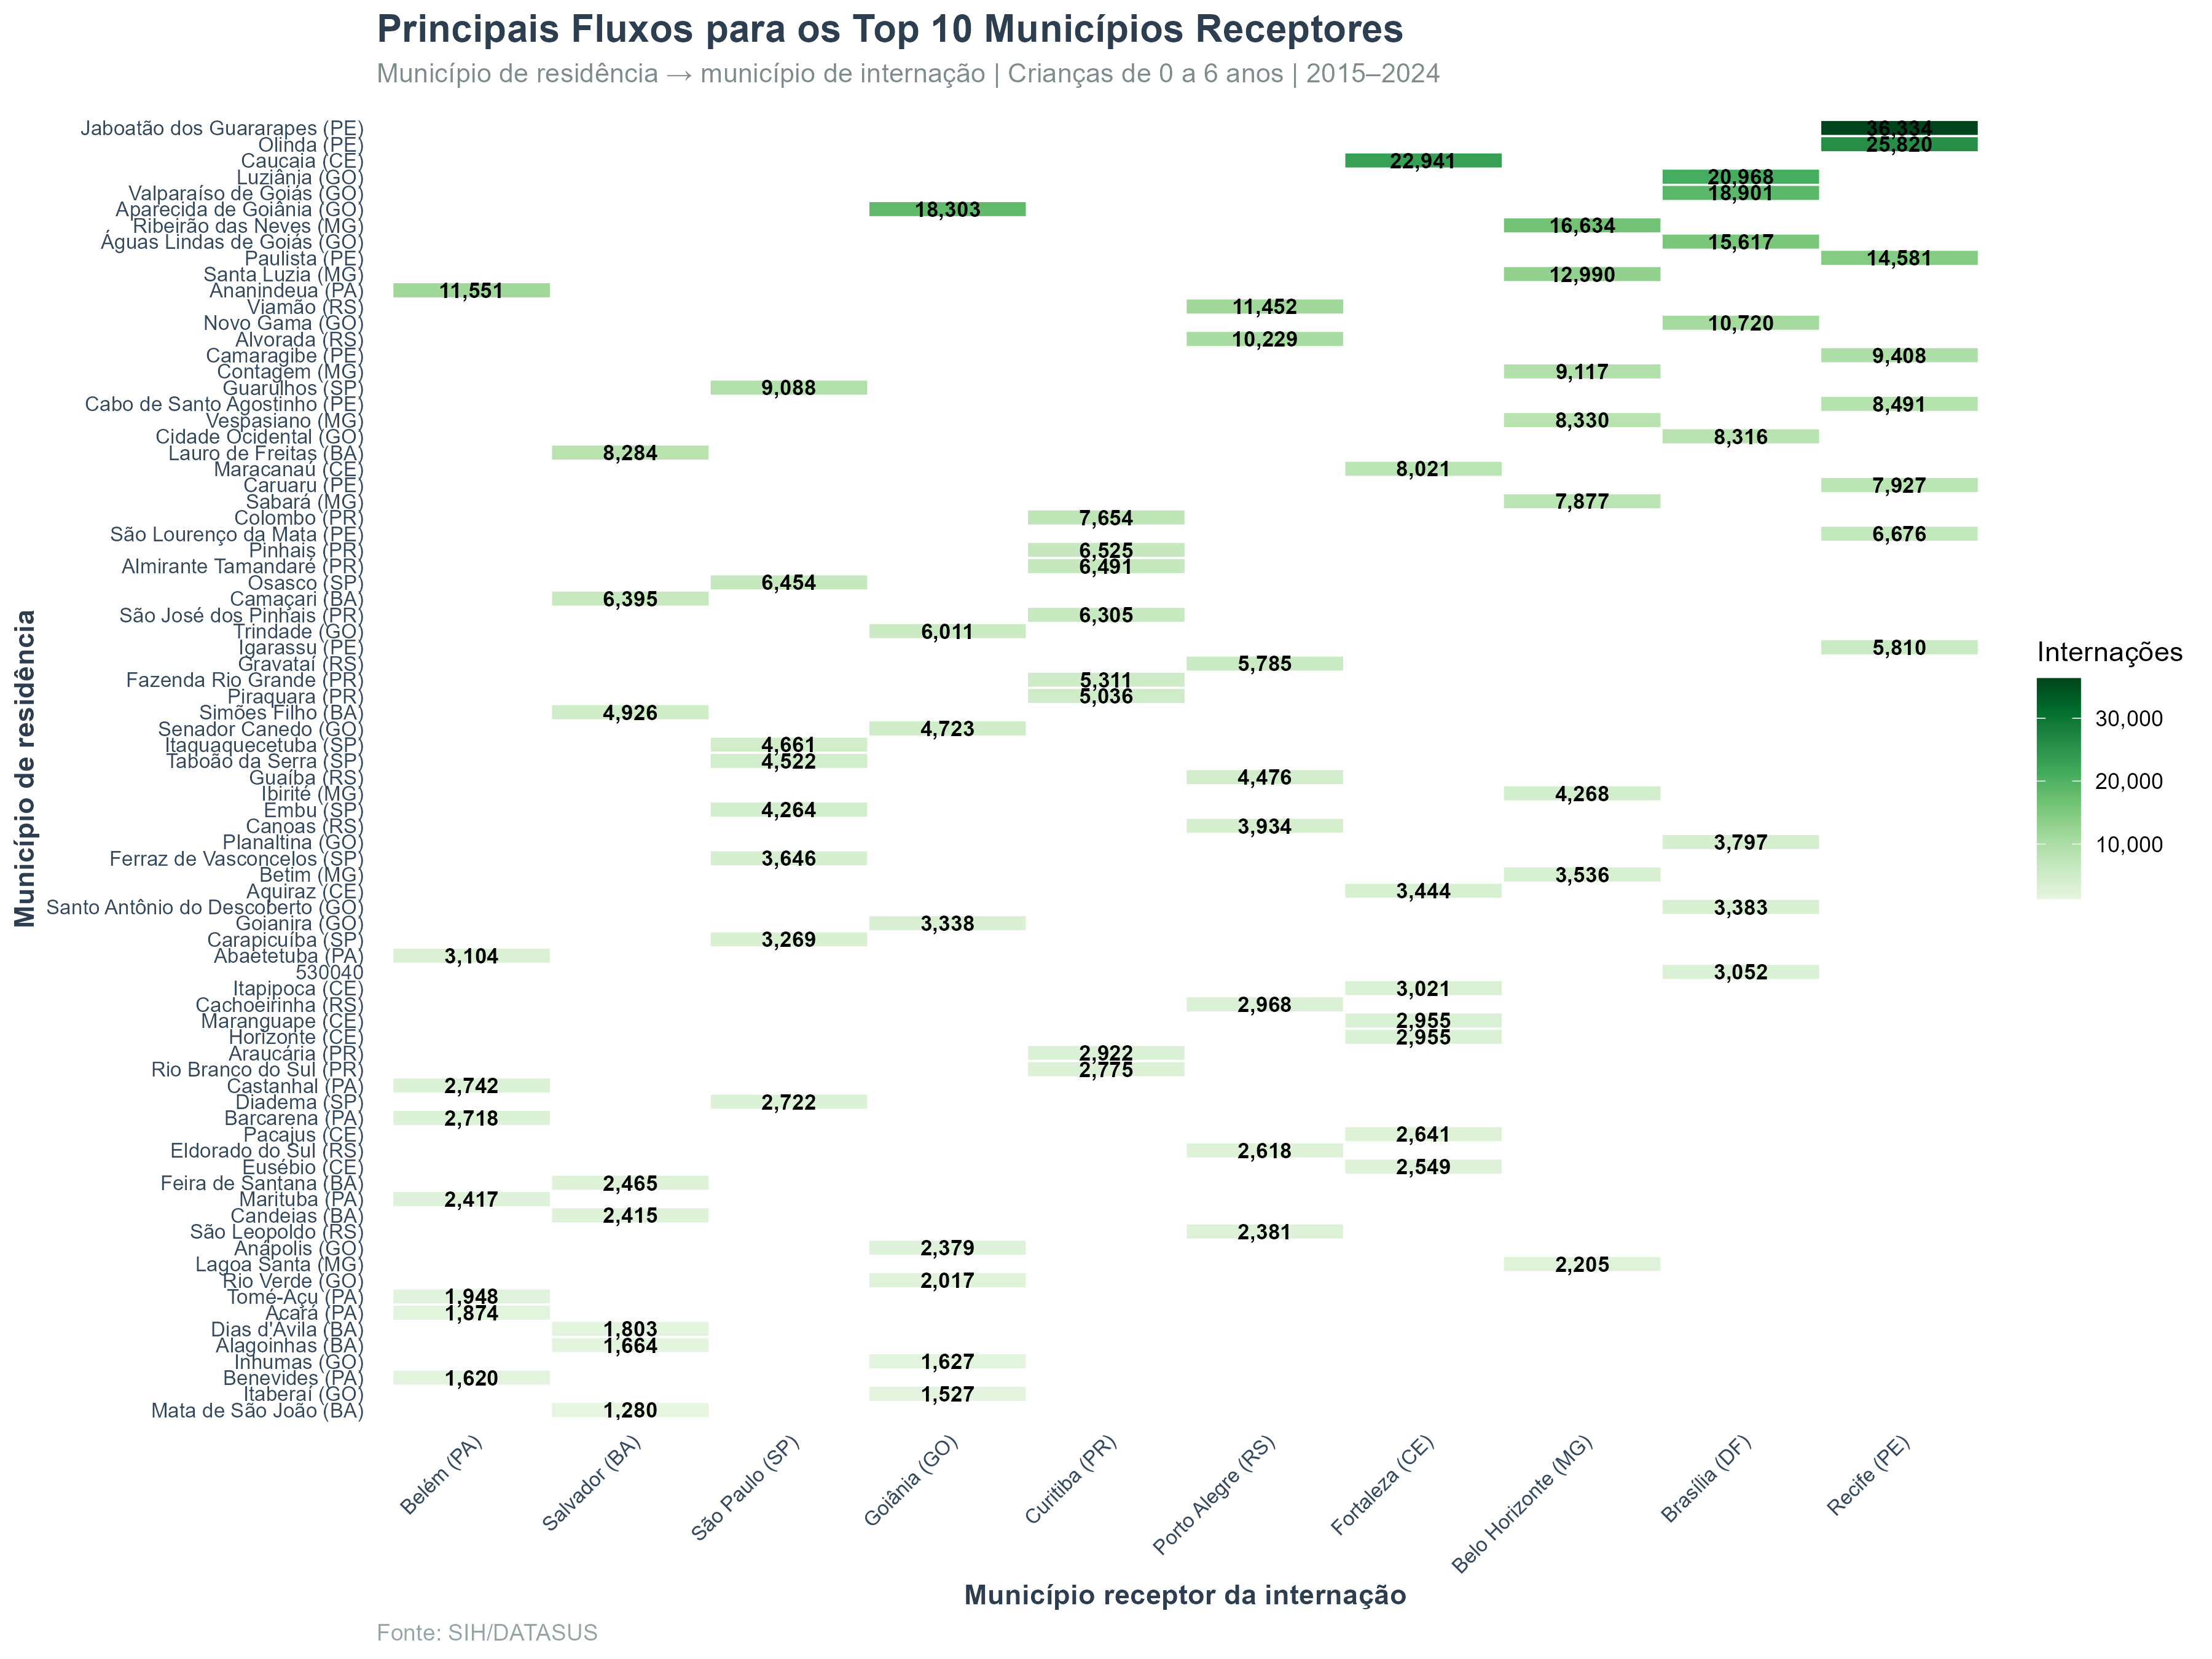
\includegraphics[width=0.9\linewidth,height=\textheight,keepaspectratio]{../outputs/SIH/Fig10_Fluxos_Top10_Municipios_Receptores_SIH.png}

}

\caption{Principais Fluxos para Municípios Mais Receptores de
Internações, 2015-2024}

\end{figure}%
\end{frame}

\begin{frame}{Óbitos Hospitalares entre Internações}
\protect\phantomsection\label{uxf3bitos-hospitalares-entre-internauxe7uxf5es}
\begin{itemize}
\tightlist
\item
  Esta análise descreve os óbitos hospitalares registrados entre
  internações de crianças de 0 a 6 anos, permitindo avaliar a magnitude
  absoluta dos óbitos em ambiente hospitalar e a letalidade hospitalar
  ao longo do período.
\end{itemize}
\end{frame}

\begin{frame}{Óbitos Hospitalares e Letalidade Hospitalar}
\protect\phantomsection\label{uxf3bitos-hospitalares-e-letalidade-hospitalar}
\begin{figure}[H]

{\centering 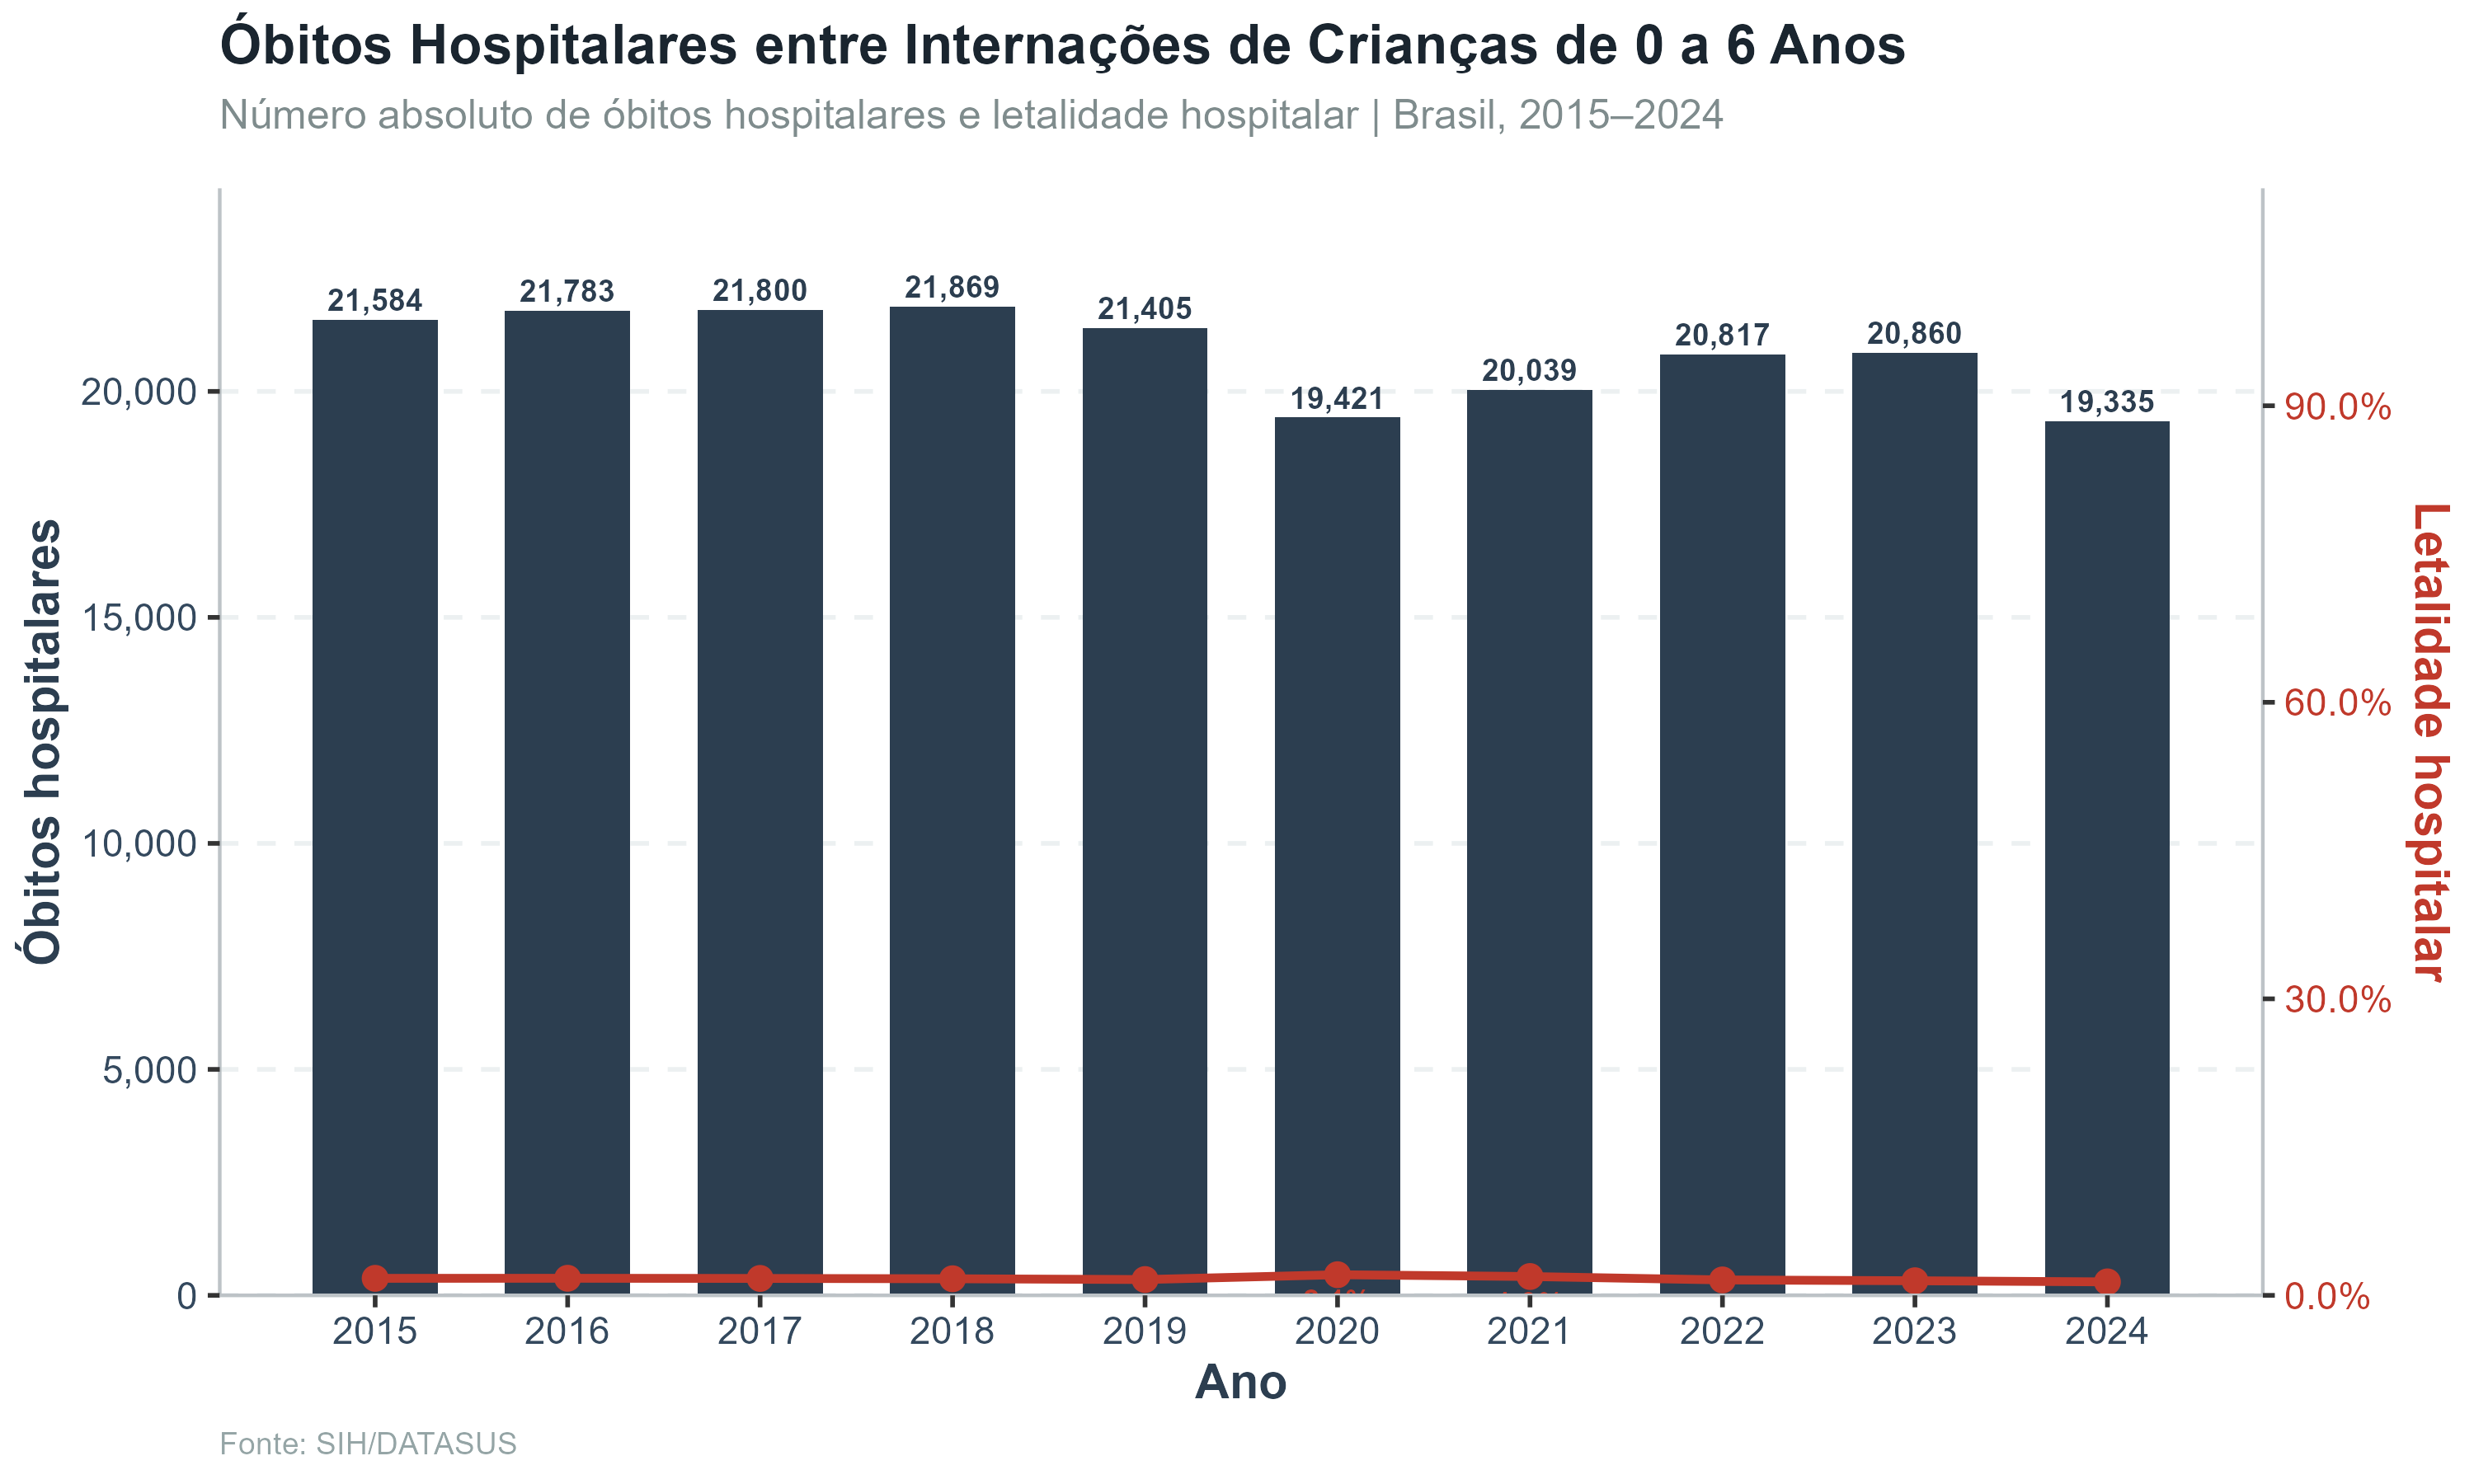
\includegraphics[width=0.6\linewidth,height=\textheight,keepaspectratio]{../outputs/SIH/Fig11_Obitos_Hospitalares_SIH.png}

}

\caption{Óbitos Hospitalares e Letalidade Hospitalar, 2015-2024}

\end{figure}%
\end{frame}

\begin{frame}{Segmentação Diagnóstica e Polos de Referência}
\protect\phantomsection\label{segmentauxe7uxe3o-diagnuxf3stica-e-polos-de-referuxeancia-1}
\begin{itemize}
\item
  Como o \textbf{CEP de residência} consta da AIH, o fluxo de origem é
  detalhado em nível de \textbf{área CEP}, e não apenas por município.\\
\item
  As afecções perinatais são analisadas em separado, e o fluxo de
  \textbf{referência terapêutica} (alta complexidade sem perinatal)
  revela a vocação de cada polo hospitalar.
\end{itemize}
\end{frame}

\begin{frame}{Segmentação Diagnóstica nos Polos}
\protect\phantomsection\label{segmentauxe7uxe3o-diagnuxf3stica-nos-polos-1}
\begin{figure}[H]

{\centering 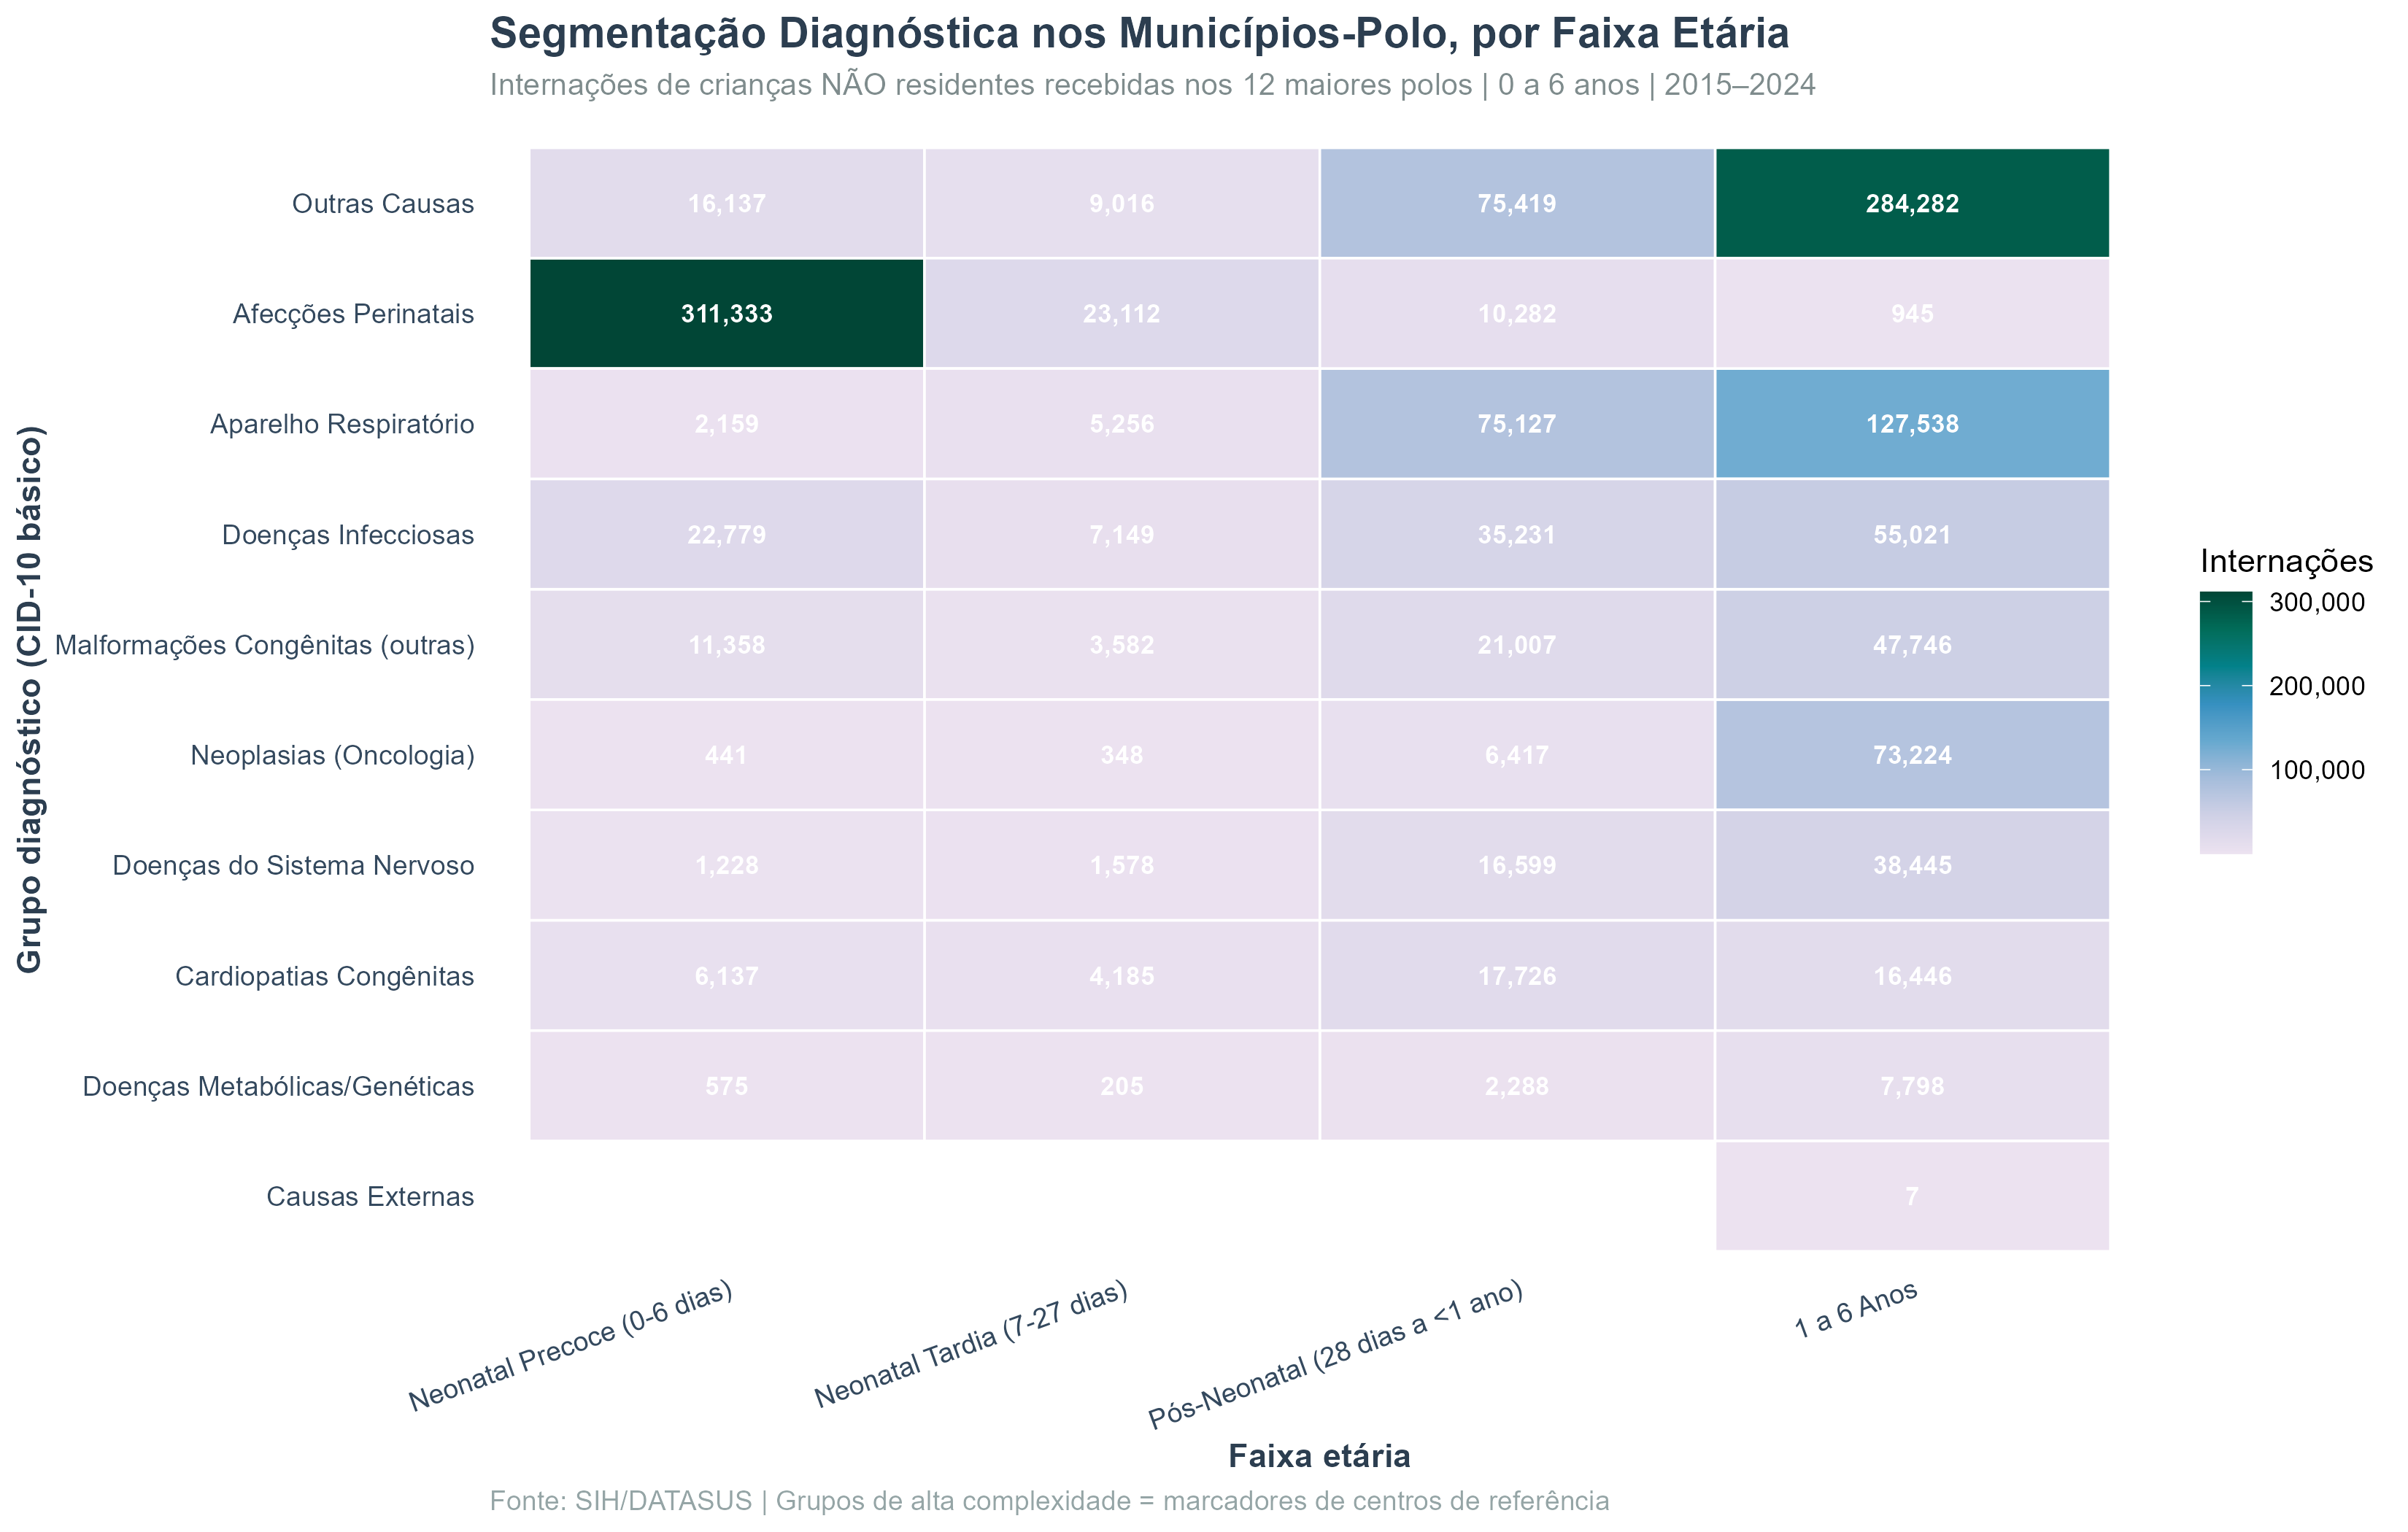
\includegraphics[width=0.9\linewidth,height=\textheight,keepaspectratio]{../outputs/SIH/Fig12_CID_Segmentado_por_Faixa_Polos_SIH.png}

}

\caption{Segmentação Diagnóstica nos Polos, por Faixa Etária}

\end{figure}%
\end{frame}

\begin{frame}{Polos por Especialidade}
\protect\phantomsection\label{polos-por-especialidade-1}
\begin{figure}[H]

{\centering 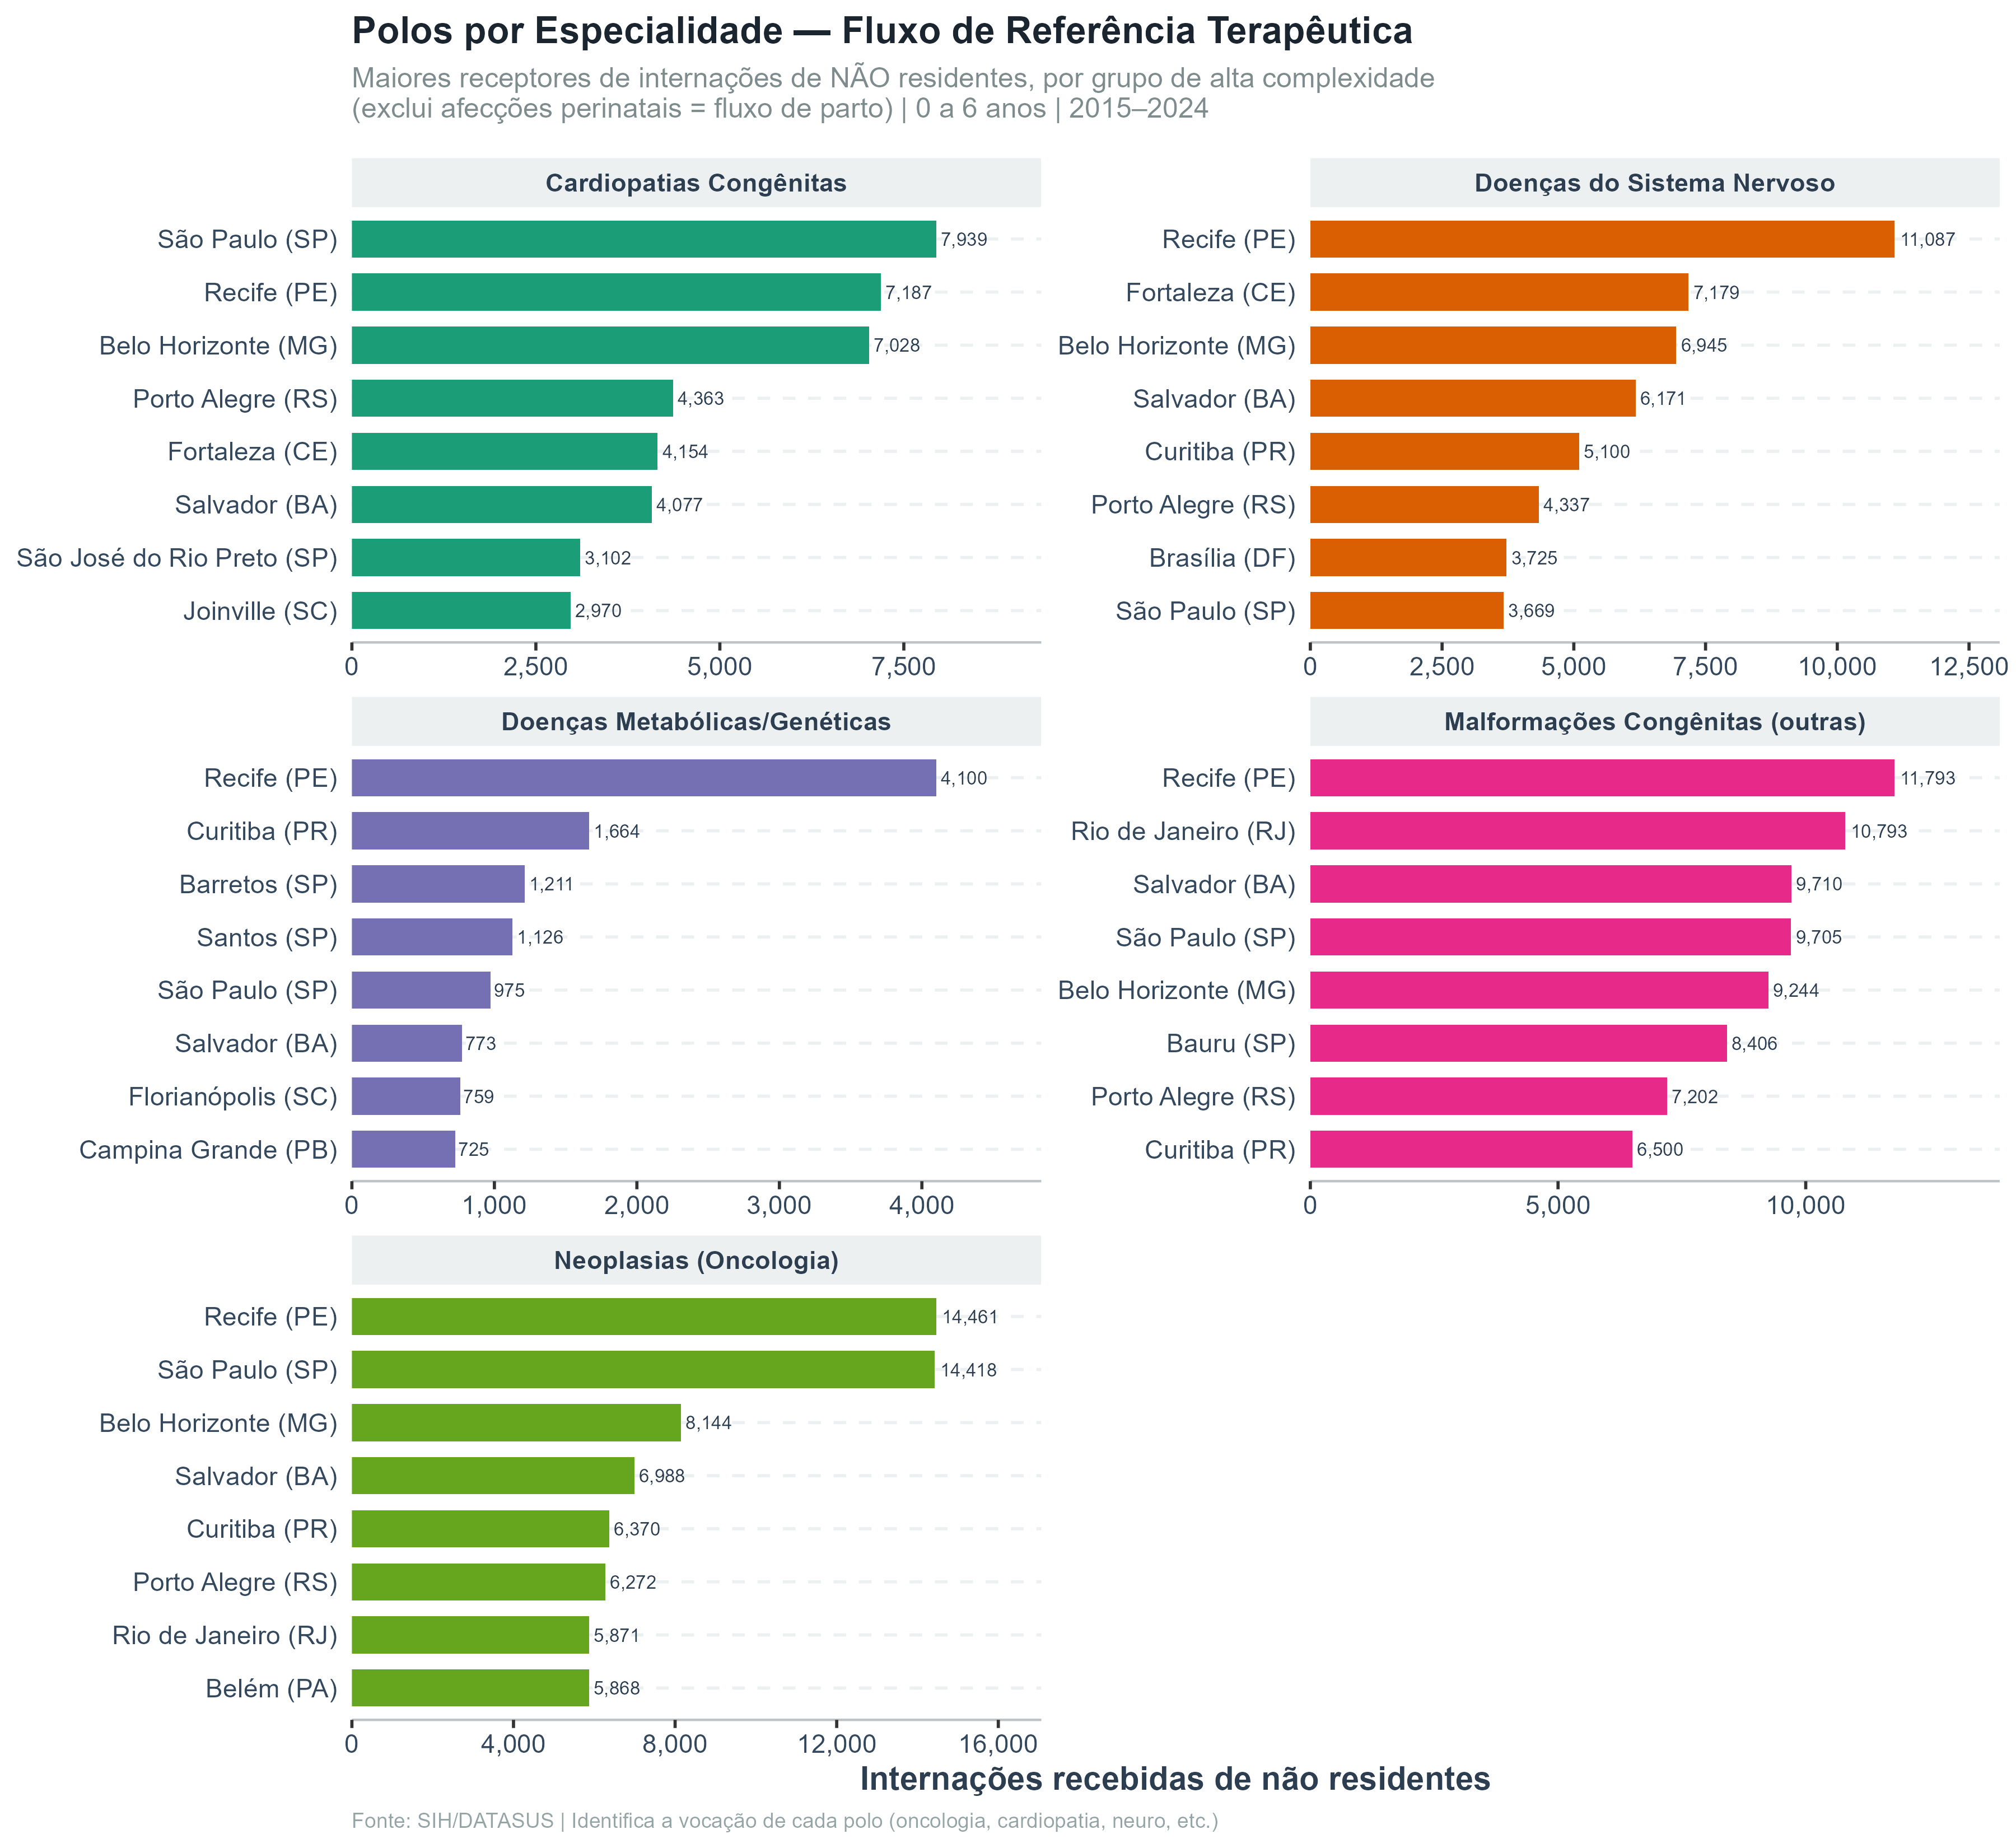
\includegraphics[width=0.6\linewidth,height=\textheight,keepaspectratio]{../outputs/SIH/Fig13_Polos_por_Especialidade_SIH.png}

}

\caption{Polos por Especialidade --- Fluxo de Referência Terapêutica}

\end{figure}%
\end{frame}

\begin{frame}{Fluxo Origem ao Polo por CEP de Residência}
\protect\phantomsection\label{fluxo-origem-ao-polo-por-cep-de-residuxeancia}
\begin{figure}[H]

{\centering 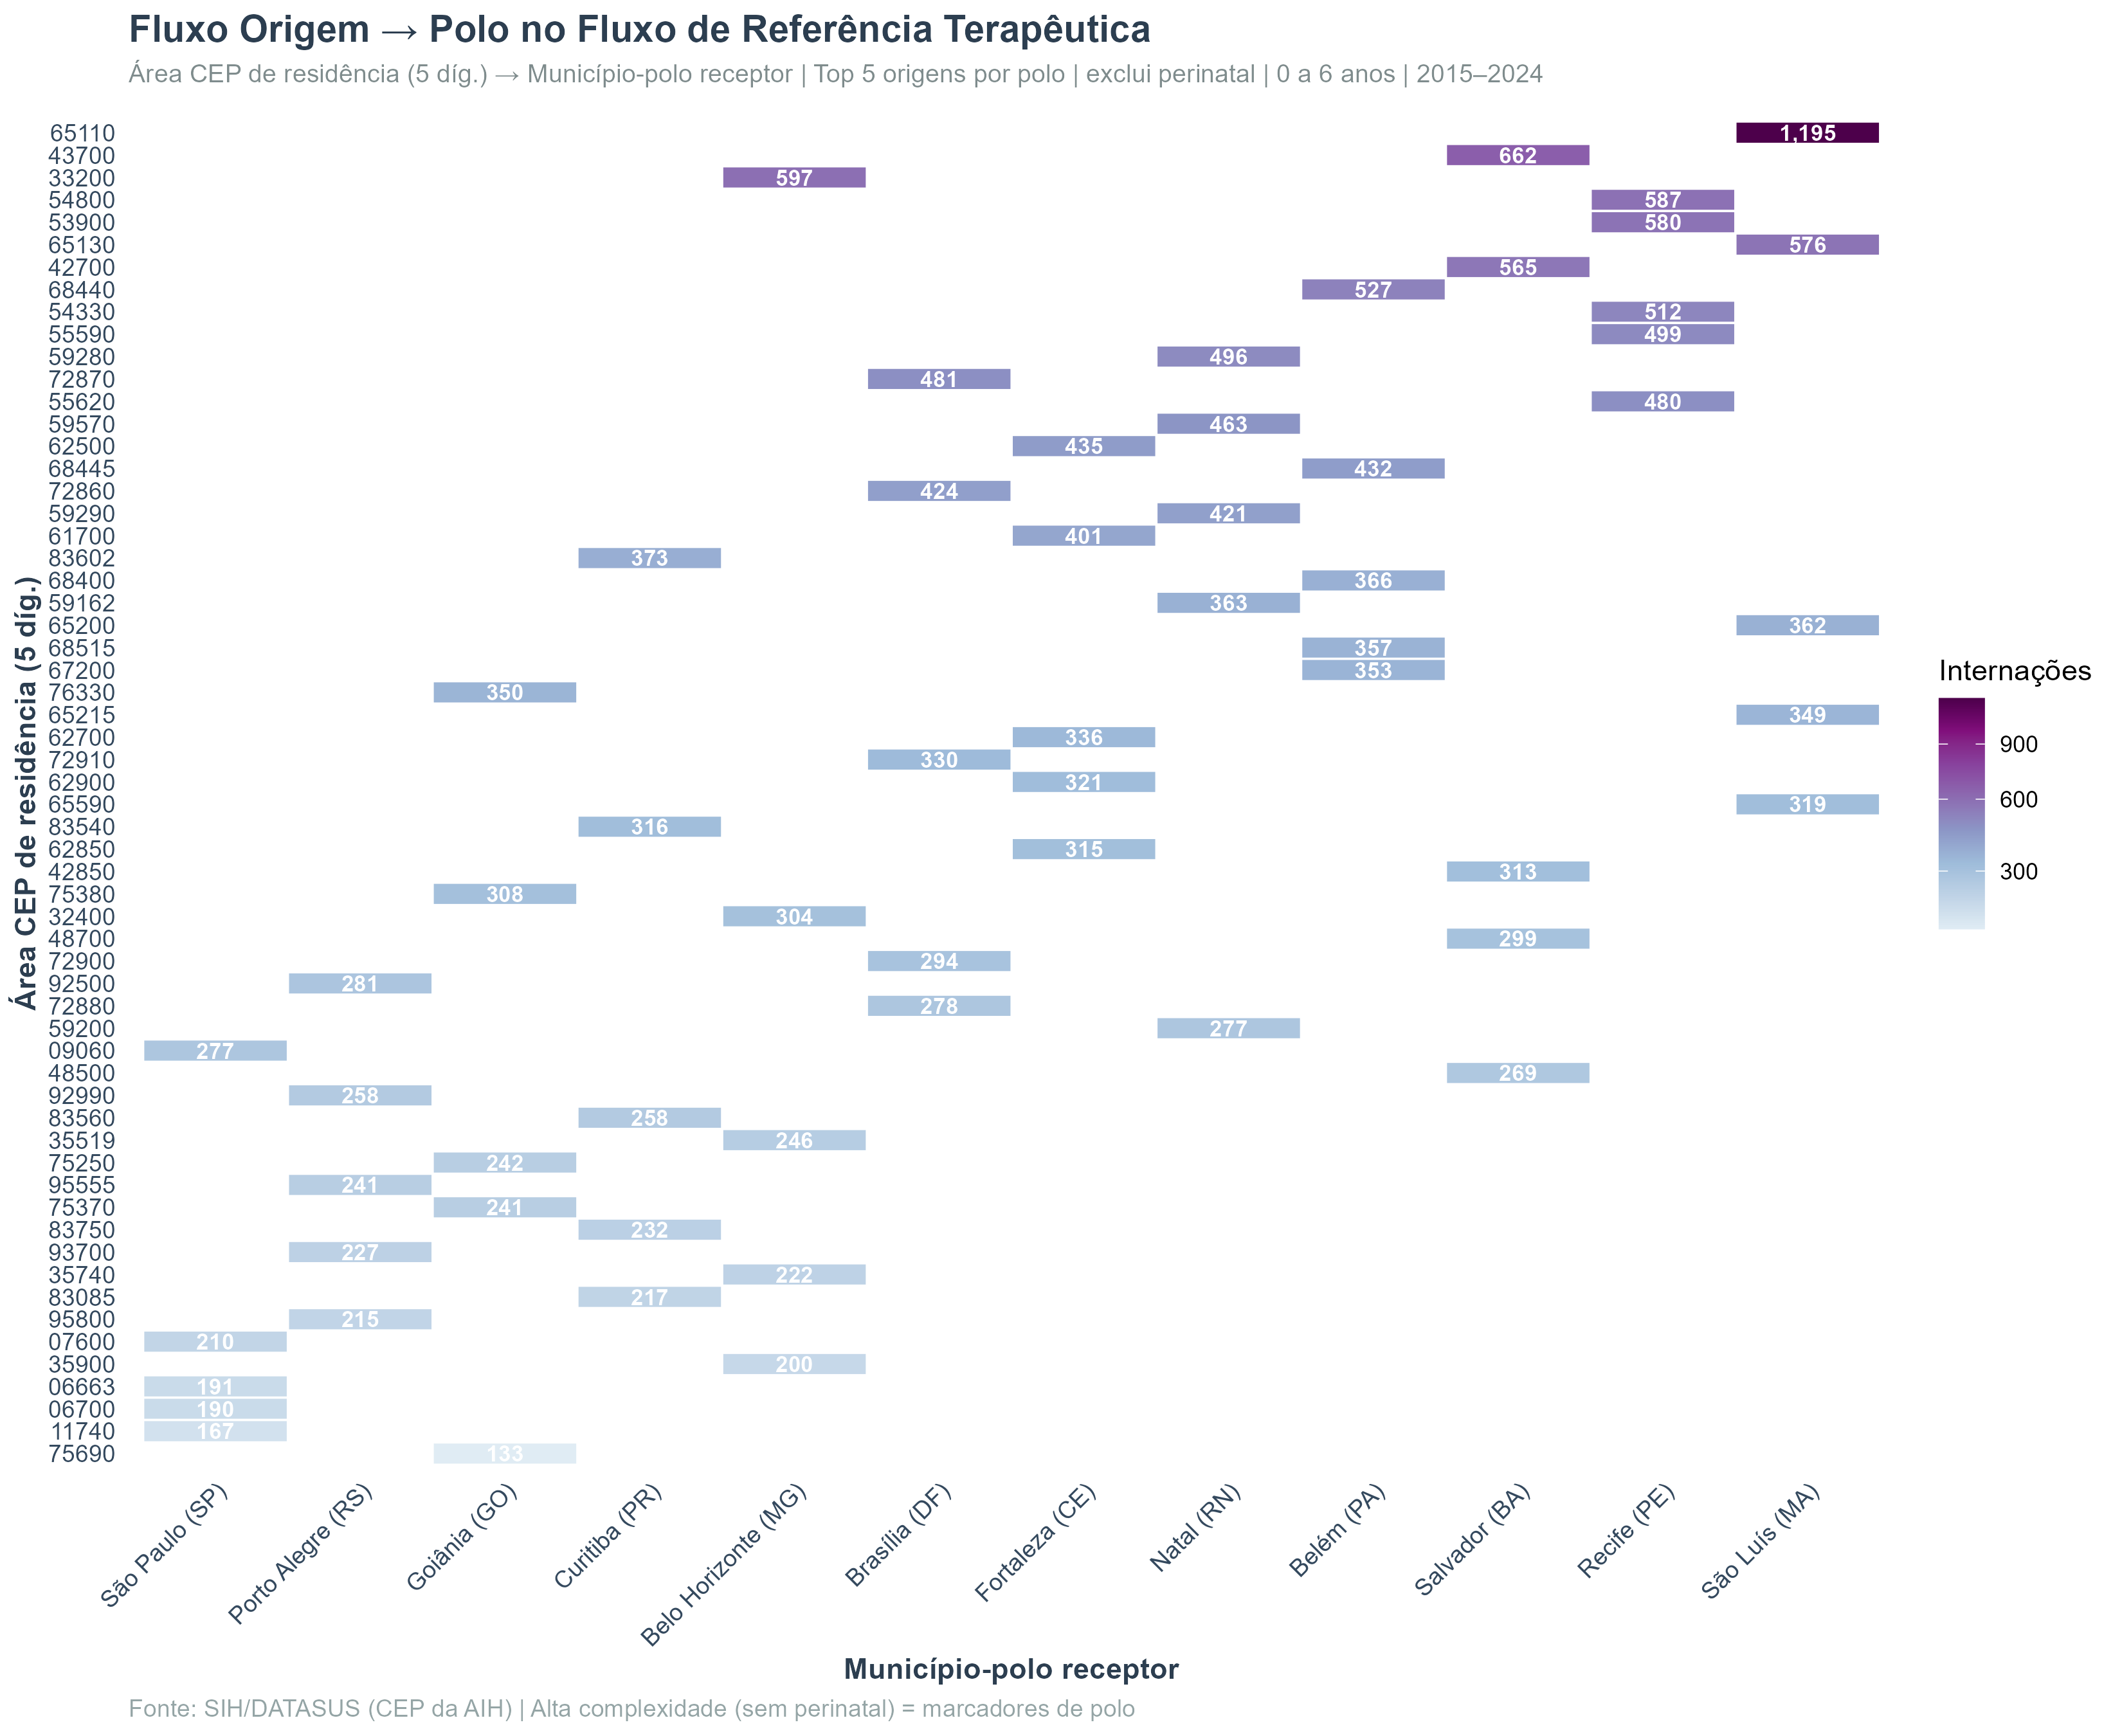
\includegraphics[width=0.6\linewidth,height=\textheight,keepaspectratio]{../outputs/SIH/Fig14_Fluxo_CEP_Origem_Destino_Polos_SIH.png}

}

\caption{Fluxo Origem ao Polo por CEP de Residência para Alta
Complexidade}

\end{figure}%
\end{frame}

\begin{frame}{Conclusão}
\protect\phantomsection\label{conclusuxe3o}
\end{frame}

\begin{frame}{Próximos Passos}
\protect\phantomsection\label{pruxf3ximos-passos}
\end{frame}

\begin{frame}{Referências}
\protect\phantomsection\label{referuxeancias}
\protect\phantomsection\label{refs}
\begin{CSLReferences}{1}{1}
\bibitem[\citeproctext]{ref-brasil2026calendario}
Brasil. Ministério da Saúde. 2026. \emph{Calendário Nacional de
Vacinação: Ano 2026 -- Ciclo de Vida: Criança (0 a 9 anos, 11 meses e 29
dias de idade)}. Ministério da Saúde.
\url{https://www.gov.br/saude/pt-br/vacinacao/calendario}.

\bibitem[\citeproctext]{ref-datasus_sim}
Brasil. Ministério da Saúde. Secretaria de Vigilância em Saúde. 2024.
\emph{Sistema de Informa{ç}{ã}o sobre Mortalidade ({SIM})}.
Coordena{ç}{ã}o-Geral de Informa{ç}{õ}es e An{á}lises Epidemiol{ó}gicas
({CGIAE}).
\url{https://svs.aids.gov.br/daent/cgiae/coesv/sistemas-informacao/sim/}.

\bibitem[\citeproctext]{ref-francca2009mortalidade}
França, Elisabeth, e Sônia Lansky. 2009. {``Mortalidade infantil
neonatal no Brasil: situa{ç}{ã}o, tend{ê}ncias e perspectivas''}.
\emph{Rede Interagencial de Informa{ç}{õ}es para Sa{ú}de, organizador.
Demografia e sa{ú}de: contribui{ç}{ã}o para an{á}lise de situa{ç}{ã}o e
tend{ê}ncias. Bras{ı́}lia: Organiza{ç}{ã}o Pan-Americana da Sa{ú}de},
83--112.

\bibitem[\citeproctext]{ref-UNIGME2024}
United Nations Inter-Agency Group for Child Mortality Estimation (UN
IGME). 2025. \emph{Levels and Trends in Child Mortality: Report 2024}.
UNICEF, World Health Organization, World Bank Group, United Nations.
\url{https://data.unicef.org/resources/levels-and-trends-in-child-mortality-2024/}.

\end{CSLReferences}
\end{frame}




\end{document}
